% Latex file containing the documentation of ADOL-C
%
% Copyright (C) Andrea Walther, Andreas Griewank, Andreas Kowarz, 
%               Hristo Mitev, Sebastian Schlenkrich, Jean Utke, Olaf Vogel 
%
% This file is part of ADOL-C. This software is provided as open source.
% Any use, reproduction, or distribution of the software constitutes 
% recipient's acceptance of the terms of the accompanying license file.
%++++++++++++++++++++++++++++++++++++++++++++++++++++++++++++++++

\documentclass[11pt,twoside]{article}
\usepackage{hyperref}
\usepackage{amsmath,amsthm,amssymb}
\usepackage{graphicx}
\usepackage{datetime}

\newdateformat{monthyear}{\monthname\ \THEYEAR}

\usepackage{color}

\pagestyle{headings} 
\bibliographystyle{plain}
\parskip=6pt

\setlength{\textwidth}{433.6pt}
\setlength{\oddsidemargin}{23pt}
\setlength{\evensidemargin}{23pt}
\setlength{\topmargin}{25.0pt}
\setlength{\textheight}{580pt}
\setlength{\baselineskip}{8pt}

\newcommand{\N}{{ {\rm I} \kern -.225em {\rm N} }}
\newcommand{\R}{{ {\rm I} \kern -.225em {\rm R} }}
\newcommand{\T}{{ {\rm I} \kern -.425em {\rm T} }}

\renewcommand{\sectionautorefname}{Section}
\renewcommand{\subsectionautorefname}{Section}
\renewcommand{\figureautorefname}{Figure}
\renewcommand{\tableautorefname}{Table}

\setcounter{equation}{0}

\newcommand{\packagename}{adolc}
\newcommand{\packageversion}{2.7.0-trunk}
\newcommand{\packagetar}{\packagename-\packageversion}


%++++++++++++++++++++++++++++++++++++++++++++++++++++++++++++++++
\begin{document}

\begin{titlepage}
\begin{center}
{\Large {\bf ADOL-C:}} 
\footnote{The development of earlier versions was supported by the Office of
  Scientific Computing, U.S. Department of Energy, the NSF, and the Deutsche
  Forschungsgemeinschaft. During the development of the current
  version Andrea Walther and Andreas Kowarz were supported by the
  grant Wa 1607/2-1 of the Deutsche Forschungsgemeinschaft}  
\vspace{0.2in} \\
%
{\Large A Package for the Automatic Differentiation}\vspace{0.1in} \\
{\Large of Algorithms Written in C/C++}\\
\vspace{.2in}
{\large\bf  Version \packageversion, \monthyear\today} \\
\bigskip
 \mbox{Andrea Walther}\footnote{Institute of Mathematics, University
   of Paderborn, 33098 Paderborn, Germany} and
 \mbox{Andreas Griewank}\footnote{Department of Mathematics,
 Humboldt-Universit\"at zu Berlin, 10099 Berlin, Germany}
\end{center}
%
%++++++++++++++++++++++++++++++++++++++++++++++++++++++++++++++++
\begin{abstract}
The C++ package ADOL-C described here facilitates the evaluation of
first and higher derivatives of vector functions that are defined
by computer programs written in C or C++. The resulting derivative
evaluation routines may be called from C, C++, Fortran, or any other
language that can be linked with C.

The numerical values of derivative vectors are obtained free
of truncation errors at a small multiple of the run time and
random access memory required by the given function evaluation program.
Derivative matrices are obtained by columns, by rows or in sparse format. 
For solution curves defined by ordinary differential equations,
special routines are provided that evaluate the Taylor coefficient vectors
and their Jacobians with respect to the current state vector.
For explicitly or implicitly defined functions derivative tensors are 
obtained with a complexity that grows only quadratically in their
degree. The derivative calculations involve a possibly substantial but
always predictable amount of data. Since the data is accessed strictly sequentially 
it can be automatically paged out to external files. 
\end{abstract}
%
{\bf Keywords}: Computational Differentiation, Automatic 
         Differentiation,
         Chain Rule, Overloading, Taylor Coefficients, 
         Gradients, Hessians, Forward Mode, Reverse Mode,
         Implicit Function Differentiation, Inverse Function Differentiation 
\medskip

\noindent
{\bf Abbreviated title}: Automatic differentiation by overloading in C++
%
\end{titlepage}
%
\tableofcontents       
%

\newpage
%
%++++++++++++++++++++++++++++++++++++++++++++++++++++++++++++++++
%
%++++++++++++++++++++++++++++++++++++++++++++++++++++++++++++++++
\section{Preparing a Section of C or C++ Code for Differentiation}
\label{prepar}
%
\subsection{Introduction}
%
\setcounter{equation}{0}
The package \mbox{ADOL-C} 
utilizes overloading in C++, but the
user has to know only C. The acronym stands for {\bf A}utomatic 
{\bf D}ifferentiation by {\bf O}ver{\bf L}oading in {\bf C}++.
In contrast to source transformation approaches, overloading does not generate intermediate
source code. 
As starting points to retrieve further information on techniques and
application of automatic differentiation, as well as on other AD
tools, we refer to the book \cite{GrWa08}. Furthermore, the web page
\verb=http://www.autodiff.org= of the AD community forms a rich source
of further information and pointers.


ADOL-C facilitates the simultaneous
evaluation of arbitrarily high directional derivatives and the
gradients of these Taylor coefficients with respect to all independent
variables. Relative to the cost of evaluating the underlying function, 
the cost for evaluating any such scalar-vector pair grows as the
square of the degree of the derivative but is still completely
independent of the numbers $m$ and $n$. 

This manual is organized as follows. This section explains the 
modifications required to convert undifferentiated code to code that 
compiles with ADOL-C. 
\autoref{tape} covers aspects of the tape of recorded data that ADOL-C uses to
evaluate arbitrarily high order derivatives. The discussion includes storage 
requirements and the tailoring of certain tape characteristics to fit specific
user needs. Descriptions of easy-to-use drivers for a  convenient derivative 
evaluation are contained in \autoref{drivers}. 
\autoref{forw_rev_ad} offers a more mathematical characterization of
the different modes of AD to compute derivatives. At the same time, the
corresponding drivers of ADOL-C are explained.  
The overloaded derivative evaluation routines using the forward and the reverse
mode of AD are explained in \autoref{forw_rev}. 
Advanced differentiation techniques as the optimal checkpointing for
time integrations, the exploitation of fixed point iterations, the usages
of external differentiated functions and the differentiation of OpenMP
parallel programs are described in \autoref{adv_ad}. 
The traceless forward mode is presented in \autoref{traceless}.
\autoref{install} details the installation and 
use of the ADOL-C package. Finally, \autoref{example} 
furnishes some example programs that incorporate the ADOL-C package to 
evaluate first and higher-order
derivatives.  These and other examples are distributed with the ADOL-C
source code.
The user should simply refer to them if the more abstract and general 
descriptions of ADOL-C provided in this document do not suffice.
%
%++++++++++++++++++++++++++++++++++++++++++++++++++++++++++++++++
\subsection{Declaring Active Variables}
%
\label{DecActVar}
%
The key ingredient of automatic differentiation by overloading is the
concept of an {\em active variable}. All variables that may be
considered as differentiable quantities at some time
during the program execution must be of an active
type. ADOL-C uses one 
active scalar type, called {\sf adouble}, whose real part is of the
standard type {\sf double}. 
Typically, one will declare the independent variables
and all quantities that directly or indirectly depend on them as 
{\em active}. Other variables that do not depend on the independent
variables but enter, for example, as parameters, may remain one of the
{\em passive} types {\sf double, float}, or {\sf int}. There is no
implicit type conversion from {\sf adouble} to any of these passive
types; thus, {\bf failure to declare variables as active when they
depend on other active variables will result in a compile-time error
message}. In data flow terminology, the set of active variable names
must contain all its successors in the dependency graph. All components
of indexed arrays must have the same activity status.

The real component of an {\sf adouble x} can be extracted as
{\sf x.value()}. In particular,
such explicit conversions are needed for the standard output procedure
{\sf printf}. The output stream operator \boldmath $\ll$ \unboldmath is overloaded such
that first the real part of an {\sf adouble} and then the string
``{\sf (a)}" is added to the stream. The input stream operator \boldmath $\gg$ \unboldmath  can
be used to assign a constant value to an {\sf adouble}.
Naturally, {\sf adouble}s may be
components of vectors, matrices, and other arrays, as well as
members of structures or classes. 

The C++ class {\sf adouble}, its member functions, and the overloaded
versions of all arithmetic operations, comparison operators, and 
most ANSI C functions are contained in the file \verb=adouble.cpp= and its
header \verb=<adolc/adouble.h>=. The latter must be included for compilation
of all program files containing {\sf adouble}s and corresponding 
operations. 
%
%++++++++++++++++++++++++++++++++++++++++++++++++++++++++++++++++
\subsection{Marking Active Sections}
\label{markingActive}
%
All calculations involving active variables that occur between
the void function calls
\begin{center}
{\sf trace\_on(tag,keep)} \hspace{0.3in} and \hspace{0.3in}
{\sf trace\_off(file)}
\end{center}
are recorded on a sequential data set called {\em tape}. Pairs of
these function calls can appear anywhere in a C++ program, but
they must not overlap. The nonnegative integer argument {\sf tag} identifies the
particular tape for subsequent function or derivative evaluations.
Unless several tapes need to be kept, ${\sf tag} =0$ may be used throughout.
The optional integer arguments {\sf keep} and
{\sf file} will be discussed in \autoref{tape}. We will refer to the
sequence of statements executed between a particular call to
{\sf trace\_on} and the following call to {\sf trace\_off} as an
{\em active section} of the code. The same active section may be
entered repeatedly, and one can successively generate several traces
on distinct tapes by changing the value of {\sf tag}. 
Both functions {\sf trace\_on} and {\sf trace\_off} are prototyped in
the header file \verb=<adolc/taputil.h>=, which is included by the header
\verb=<adolc/adouble.h>= automatically.

Active sections may contain nested or even recursive calls to functions
provided by the user. Naturally, their formal and actual parameters
must have matching types. In particular, the functions must be 
compiled with their active variables declared as
{\sf adouble}s and with the header file \verb=<adolc/adouble.h>= included.  
Variables of type {\sf adouble} may be declared outside an active section and need not
go out of scope before the end of an active section. 
It is not necessary -- though desirable -- that free-store {\sf adouble}s
allocated within
an active section be deleted before its completion. The values of all
{\sf adouble}s that exist at the beginning and end of an active section
are automatically 
recorded by {\sf trace\_on} and {\sf trace\_off}, respectively.
%
%++++++++++++++++++++++++++++++++++++++++++++++++++++++++++++++++
\subsection{Selecting Independent and Dependent Variables}
%
One or more active variables that are read in or initialized to
the values of constants or passive variables must be distinguished as
independent variables. Other active variables that are similarly 
initialized may be considered as temporaries (e.g., a variable that
accumulates the partial sums of a scalar product after being 
initialized to zero). In order to distinguish an active variable {\sf x} as
independent, ADOL-C requires an assignment of the form
\begin{center}
{\sf x} \boldmath $\ll=$ \unboldmath {\sf px}\hspace{0.2in}// {\sf px} of any passive numeric type $\enspace .$
\end{center}
This special initialization ensures that {\sf x.value()} = {\sf px}, and it should
precede any other assignment to {\sf x}. However, {\sf x} may be reassigned
other values subsequently. Similarly, one or more active variables {\sf y}
must be distinguished as dependent by an assignment of the form
\begin{center}
{\sf y \boldmath $\gg=$ \unboldmath py}\hspace{0.2in}// {\sf py} of any  passive type $\enspace ,$ 
\end{center}
which ensures that {\sf py} = {\sf y.value()} and should not be succeeded 
by any other assignment to {\sf y}. However, a dependent variable {\sf y} 
may have been assigned other real values previously, and it could even be an 
independent variable as well.  The derivative values calculated after
the
completion of an active section always represent {\bf derivatives of the final 
values of the dependent variables with respect to the initial values of the
independent variables}. 

The order in which the independent and dependent variables are marked
by the \boldmath $\ll=$ \unboldmath and \boldmath $\gg=$ \unboldmath statements matters crucially for the subsequent
derivative evaluations. However, these variables do not have to be
combined into contiguous vectors. ADOL-C counts the number of
independent and dependent variable specifications within each active
section and records them in the header of the tape.
%
%++++++++++++++++++++++++++++++++++++++++++++++++++++++++++++++++
\subsection{A Subprogram as an Active Section} 
%
As a generic example let us consider a C(++) function of the form
shown in \autoref{code1}.
%
\begin{figure}[hbt]
\framebox[\textwidth]{\parbox{\textwidth}{
\begin{center}
\begin{tabbing}
{\sf void eval(}\= {\sf int n, int m,} \hspace{0.5 in} \=  // number of independents and dependents\\
\>{\sf  double *x,} \> // independent variable vector \\
\>{\sf  double *y,} \> // dependent variable vector  \\ 
\> {\sf int *k, } \> // integer parameters \\ 
\>{\sf  double *z)}  \> // real parameters \\
{\sf \{ }\hspace{0.1 in } \=  \> // beginning of function body \\
\>{\sf double t = 0;}  \> // local variable declaration \\
\>{\sf  for (int i=0; i \boldmath $<$ \unboldmath n; i++)} \> // begin of computation \\
\>\hspace{0.2in}{\sf  t += z[i]*x[i];} \> //  continue  \\
\>{\sf  $\cdots \cdots \cdots \cdots $} \> // continue \\
\>{\sf  y[m-1] = t/m; }   \> //   end of computation \\
{\sf  \} } \>  \> // end of function 
\end{tabbing}
\end{center}
}} 
\caption{Generic example of a subprogram to be activated}
\label{code1}
\end{figure}
%

If {\sf eval} is to be called from within an active C(++)
section with {\sf x}
and {\sf y} as vectors of {\sf adouble}s and the other parameters
passive, then one merely has to change the type declarations of all
variables that depend on {\sf x} from {\sf double} or {\sf float} to
{\sf adouble}. Subsequently, the subprogram must be compiled with the
header file \verb=<adolc/adouble.h>= included as described
in \autoref{DecActVar}. Now let us consider the situation when {\sf eval} is
still to be called with integer and real arguments, possibly from
a program written in Fortran77, which  does not allow overloading. 

To automatically compute derivatives of the dependent 
variables {\sf y} with respect to the independent variables {\sf x}, we
can make the body of the function into an active section. For
example, we may modify the previous program segment 
as in \autoref{adolcexam}.
The renaming and doubling up of the original independent and dependent
variable vectors by active counterparts may seem at first a bit clumsy.
However, this transformation has the advantage that the calling
sequence and the computational part, i.e., where the function is
really evaluated, of {\sf eval} remain completely
unaltered. If the temporary variable {\sf t} had remained a {\sf double},
the code would not compile, because of a type conflict in the assignment
following the declaration. More detailed example codes are listed in 
\autoref{example}.

\begin{figure}[htb]
\framebox[\textwidth]{\parbox{\textwidth}{
\begin{center}
\begin{tabbing}
{\sf void eval(} \= {\sf  int n,m,} \hspace{1.0 in}\= // number of independents and dependents\\
\> {\sf double *px,} \> // independent passive variable vector \\
\> {\sf double *py,} \> // dependent passive variable vector  \\ 
\> {\sf int *k,}  \> // integer parameters \\
\> {\sf double *z)} \> // parameter vector \\
{\sf \{}\hspace{0.1 in}\= \> // beginning of function body \\
\>{\sf  short int tag = 0;} \>   // tape array and/or tape file specifier\\
\>{\sf trace\_on(tag);} \> // start tracing  \\
\>{\sf adouble *x, *y;} \> // declare active variable pointers \\
\>{\sf x = new adouble[n];}\>// declare active independent variables \\ 
\>{\sf y = new adouble[m];} \> // declare active dependent variables \\
\>{\sf  for (int i=0; i \boldmath $<$ \unboldmath n; i++)} \\
\>\hspace{0.2in} {\sf x[i] \boldmath $\ll=$ \unboldmath  px[i];} \> // select independent variables \\
\>{\sf adouble t = 0;}  \> // local variable declaration \\
     \>{\sf  for (int i=0; i \boldmath $<$ \unboldmath n; i++)} \> //  begin crunch \\
     \>\hspace{0.2in}{\sf  t += z[i]*x[i];} \> //  continue crunch \\
     \>{\sf  $\cdots \cdots \cdots \cdots $} \> // continue crunch \\
     \>{\sf  $\cdots \cdots \cdots \cdots $} \> // continue crunch \\
     \>{\sf  y[m-1] = t/m; }   \> //   end crunch as before\\
     \>{\sf for (int j=0; j \boldmath $<$ \unboldmath m; j++)} \\
     \>\hspace{0.2in}{\sf y[j] \boldmath $\gg=$ \unboldmath py[j];} \> // select dependent variables \\
     \>{\sf  delete[] y;} \>// delete dependent active variables \\
     \>{\sf  delete[] x;} \>// delete independent active variables \\
     \>{\sf trace\_off();} \> // complete tape \\
{\sf  \}}   \>\> // end of function 
\end{tabbing} 
\end{center}}}
\caption{Activated version of the code listed in \autoref{code1}}
\label{adolcexam}
\end{figure}
%
%++++++++++++++++++++++++++++++++++++++++++++++++++++++++++++++++
\subsection{Overloaded Operators and Functions}
\label{OverOper}
%
As in the subprogram discussed above, the actual computational
statements of a C(++) code need not be altered for the purposes of
automatic differentiation. All arithmetic operations, as well as the
comparison and assignment operators, are overloaded, so any or all of
their operands can be an active variable. An {\sf adouble x} occurring
in a comparison operator is effectively replaced by its real value
{\sf x.value()}. Most functions contained in the ANSI C standard for 
the math library are overloaded for active arguments. The only 
exceptions are the non-differentiable functions {\sf fmod} and 
{\sf modf}. Otherwise, legitimate C code in active sections can remain
completely unchanged, provided the direct output of active variables
is avoided. The rest of this subsection may be skipped by first time
users who are not worried about marginal issues of differentiability
and efficiency. 

The modulus {\sf fabs(x)} is everywhere Lipschitz continuous but not
properly differentiable at the origin, which raises the question of
how this exception ought to be handled. Fortunately, one can easily
see that {\sf fabs(x)} and all its compositions with smooth
functions are still directionally differentiable. These
directional derivatives of arbitrary order can be propagated in the
forward mode without any ambiguity. In other words, the forward mode as
implemented in ADOL-C  computes Gateaux derivatives
in certain directions, which reduce to Fr\'echet derivatives only
if the dependence on the direction is linear. Otherwise,
the directional derivatives are merely positively homogeneous with
respect to the scaling of the directions.
For the reverse mode, ADOL-C sets the derivative of {\sf fabs(x)} at
the origin somewhat arbitrarily to zero.

We have defined binary functions {\sf fmin} and {\sf fmax} for {\sf adouble}
arguments, so that function and derivative values are obtained consistent
with those of {\sf fabs} according to the identities
\[
 \min(a,b) = [a+b-|a-b|]/2 \quad {\rm and} \quad
 \max(a,b) = [a+b+|a-b|]/2 \quad . 
\]
These relations cannot hold if either $a$ or $b$ is infinite, in which
case {\sf fmin} or {\sf fmax} and their derivatives may still be well
defined. It should be noted that the directional differentiation of
{\sf fmin} and {\sf fmax} yields at ties $a=b$ different results from
the corresponding assignment based on the sign of $a-b$. For example,
the statement 
\begin{center}
 {\sf if (a $<$ b) c = a; else c = b;}
\end{center} 
yields for {\sf a}~=~{\sf b} and {\sf a}$^\prime < $~{\sf b}$^\prime$
the incorrect directional derivative value 
{\sf c}$^\prime = $~{\sf  b}$^\prime$ rather than the correct
{\sf c}$^\prime = $~{\sf  a}$^\prime$. Therefore this form of conditional assignment
should be avoided by use of the function $\sf fmin(a,b)$. There
are also versions of {\sf fmin} and {\sf fmax} for two passive 
arguments and mixed passive/active arguments are handled by 
implicit conversion. 
On the function class obtained by composing the modulus with real
analytic functions, the concept of directional differentiation can be
extended to the propagation of unique one-sided Taylor expansions.
The branches taken by {\sf fabs, fmin}, and {\sf fmax}, are recorded 
on the tape. 

The functions {\sf sqrt}, {\sf pow}, and some inverse trigonometric
functions have infinite slopes at the boundary points of their domains.
At these marginal points the derivatives are set by ADOL-C to 
either {\sf $\pm$InfVal}, 0
or {\sf NoNum}, where {\sf InfVal} and {\sf NoNum} are user-defined 
parameters, see \autoref{Customizing}.
On IEEE machines {\sf InfVal} can be set to the special value 
{\sf Inf}~=~$1.0/0.0$ and {\sf NoNum} to {\sf NaN}~=~$0.0/0.0$.
For example, at {\sf a}~=~0 the first derivative {\sf b}$^\prime$ 
of {\sf b}~=~{\sf sqrt(a)} is set to 
\[
{\sf b}^\prime = \left\{
\begin{array}{ll}
\sf InfVal&\mbox{if}\;\; {\sf a}^\prime>0  \\
0&\mbox{if}\;\;{\sf a}^\prime =0 \\
\sf NoNum&\mbox{if}\;\;{\sf a}^\prime <0\\
\end{array} \right.  \enspace .
\]
In other words, we consider {\sf a} and
consequently {\sf b}  as a constant when {\sf a}$^\prime$ or more generally
all computed Taylor coefficients are zero. 

The general power function ${\sf pow(x,y)=x^y}$ is computed whenever
it is defined for the corresponding {\sf double} arguments. If {\sf x} is
negative, however, the partial derivative with respect to an integral exponent
is set to zero. 
%Similarly, the partial of {\bf pow} with respect to both arguments
%is set to zero at the origin, where both arguments vanish.     
The derivatives of the step functions 
{\sf floor}, {\sf ceil}, {\sf frexp}, and {\sf ldexp} are set to zero at all
arguments {\sf x}. The result values of the step functions 
are recorded on the tape and can later be checked to recognize 
whether a step to another level was taken during a forward sweep 
at different arguments than at taping time.

Some C implementations supply other special
functions, in particular the error function {\sf erf(x)}. For the
latter, we have included an {\sf adouble} version in \verb=<adouble.cpp>=, which
has been commented out for systems on which the {\sf double} valued version
is not available. The increment and decrement operators {\sf ++}, \boldmath $--$ \unboldmath (prefix and
postfix) are available for {\sf adouble}s.
%
% XXX: Vector and matrix class have to be reimplemented !!!
%
% and also the 
%active subscripts described in the \autoref{act_subscr}. 
Ambiguous statements like {\sf a += a++;} must be 
avoided because the compiler may sequence the evaluation of the
overloaded
expression differently from the original in terms of {\sf double}s.

As we have indicated above, all subroutines called with active arguments
must be modified or suitably overloaded. The simplest procedure is
to declare the local variables of the function as active so that
their internal calculations are also recorded on the tape.
Unfortunately, this approach is likely to be unnecessarily inefficient
and inaccurate if the original subroutine evaluates a special function
that is defined as the solution of a particular mathematical problem.
The most important examples are implicit functions, quadratures,
and solutions of ordinary differential equations. Often
the numerical methods for evaluating such special functions are
elaborate, and their internal workings are not at all differentiable in
the data. Rather than differentiating through such an adaptive
procedure, one can obtain first and higher derivatives directly from
the mathematical definition of the special function. Currently this
direct approach has been implemented only for user-supplied quadratures
as described in \autoref{quadrat}.
%
%++++++++++++++++++++++++++++++++++++++++++++++++++++++++++++++++
\subsection{Reusing the Tape for Arbitrary Input Values}
\label{reuse_tape}
%
In some situations it may be desirable to calculate the value and
derivatives of a function at arbitrary arguments by using a tape of
the function evaluation at one argument and reevaluating the
function  and its derivatives using the given ADOL-C
routines. This approach can
significantly reduce run times, and it 
also allows to port problem functions, in the form of the  
corresponding tape files, into a computing environment that
does not support C++ but does support C or Fortran.  
Therefore, the routines provided by ADOL-C for the evaluation of derivatives
can be used to at arguments $x$ other than the
point at which the tape was generated, provided there are
no user defined quadratures and all comparisons involving
{\sf adouble}s yield the same result. The last condition 
implies that the control flow is unaltered by the change
of the independent variable values. Therefore, this sufficient
condition is tested by ADOL-C and if it is not met 
the ADOL-C routine called for derivative calculations indicates this
contingency through its return value. Currently, there are six return values,
see \autoref{retvalues}. 
\begin{table}[h]
\center\small
\begin{tabular}{|r|l|}\hline
 +3 &
\begin{minipage}{12.5cm}
\vspace*{1ex}
The function is locally analytic.
\vspace*{1ex}
\end{minipage} \\ \hline
 +2 &
\begin{minipage}{12.5cm}
\vspace*{1ex}
The function is locally analytic but the sparsity
structure (compared to the situation at the  taping point)
may have changed, e.g. while at taping arguments
{\sf fmax(a,b)} returned {\sf a} we get {\sf b} at
the argument currently used.
\vspace*{1ex}
\end{minipage} \\ \hline
 +1 &
\begin{minipage}{12.5cm}
\vspace*{1ex}
At least one of the functions {\sf fmin}, {\sf fmax} or {\sf fabs}
is  evaluated at a tie or zero, respectively.  Hence, the function to be differentiated is
Lipschitz-continuous but possibly non-differentiable.
\vspace*{1ex}
\end{minipage} \\ \hline
 0 &
\begin{minipage}{12.5cm}
\vspace*{1ex}
Some arithmetic comparison involving {\sf adouble}s yields a tie.
Hence, the function to be differentiated  may be discontinuous.
\vspace*{1ex}
\end{minipage} \\ \hline
 -1 &
\begin{minipage}{12.5cm}
\vspace*{1ex}
An {\sf adouble} comparison yields different results
from the evaluation point at which the tape was generated.
\vspace*{1ex}
\end{minipage} \\ \hline
 -2 &
\begin{minipage}{12.5cm}
\vspace*{1ex}
The argument of a user-defined quadrature has changed
from the evaluation point at which the tape was generated.
\vspace*{1ex}
\end{minipage} \\ \hline
\end{tabular}
\caption{Description of return values}
\label{retvalues}
\end{table}                            

\begin{figure}[h]
\centering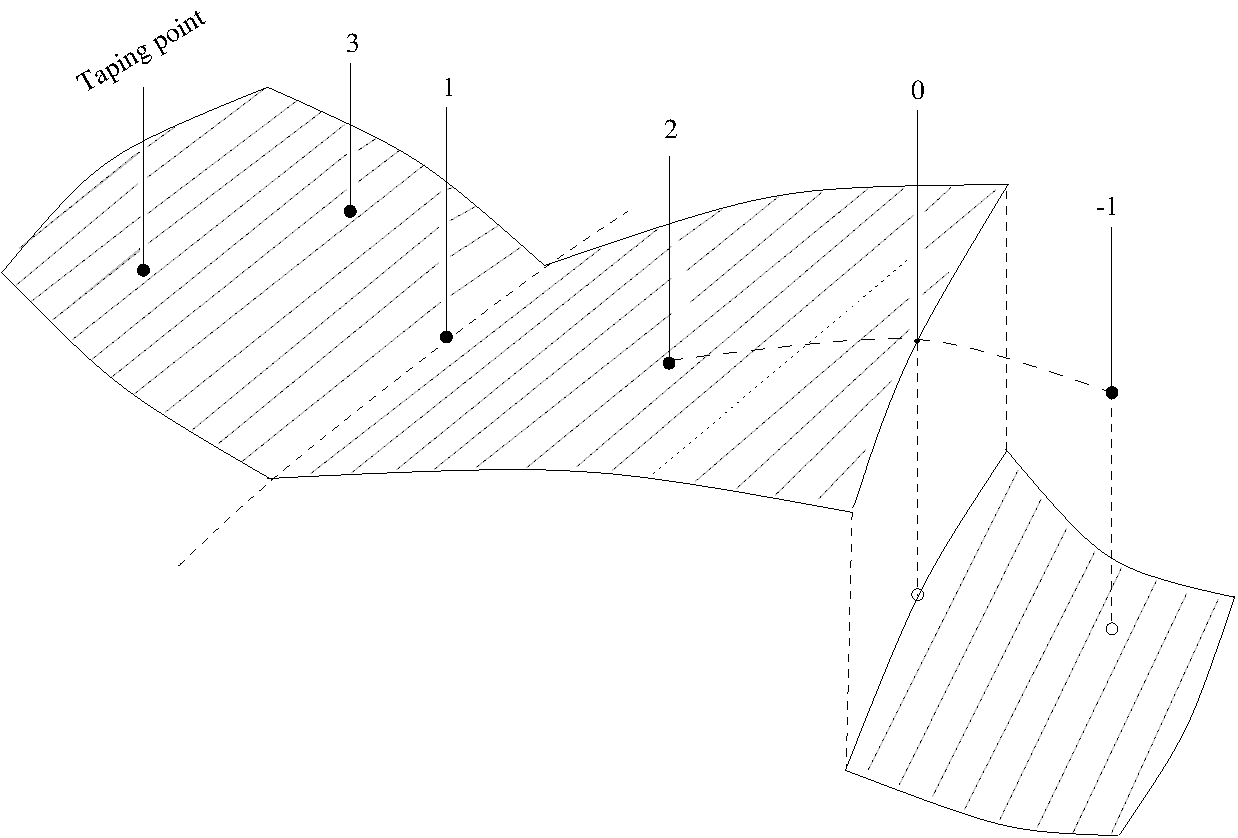
\includegraphics[width=10.0cm]{tap_point}
\caption{Return values around the taping point}
\label{fi:tap_point}
\end{figure}          

In \autoref{fi:tap_point} these return values are illustrated.
If the user finds the return value of an ADOL-C routine to be negative the
taping process simply has to be repeated by executing the active section again.
The crux of the problem lies in the fact that the tape records only
the operations that are executed during one particular evaluation of the 
function.
It also has no way to evaluate integrals since the corresponding
quadratures are never recorded on the tape. 
Therefore, when there are user-defined quadratures the retaping is necessary at each
new point. If there are only branches conditioned on {\sf adouble}
comparisons one may hope that re-taping becomes unnecessary when
the points settle down in some small neighborhood, as one would 
expect for example in an iterative equation solver. 
%
%++++++++++++++++++++++++++++++++++++++++++++++++++++++++++++++++
\subsection{Conditional Assignments}
\label{condassign}
%
It appears unsatisfactory that, for example, a simple table lookup 
of some physical property forces the re-recording of a possibly 
much larger calculation. However, the basic philosophy of ADOL-C 
is to overload arithmetic, rather than to generate a new program
with jumps between ``instructions'', which would destroy the 
strictly sequential tape access and
require the infusion of substantial compiler technology. 
Therefore, we introduce the two constructs of conditional
assignments and active integers as partial remedies to the
branching problem. 

In many cases, the functionality of branches 
can be replaced by conditional assignments.  
For this purpose, we provide a special function called
{\sf condassign(a,b,c,d)}. Its calling sequence corresponds to the 
syntax of the conditional assignment
\begin{center}
    {\sf a = (b \boldmath $>$ \unboldmath 0) ? c : d;}  
\end{center}
which C++ inherited from C. However, here the arguments are restricted to be
active or passive scalar arguments, and all expression arguments
are evaluated before the test on {\sf  b}, which is different from
the usual conditional assignment or the code segment.

Suppose the original program contains the code segment
\begin{center}
{\sf if (b \boldmath $>$ \unboldmath 0) a = c; else a = d;}\\
\end{center}
Here, only one of the expressions (or, more generally, program blocks)
{\sf c} and {\sf d} is evaluated, which exactly constitutes the problem
for ADOL-C. To obtain the correct value {\sf a} with ADOL-C, one
may first execute both branches and then pick either {\sf c}
or {\sf d} using 
{\sf condassign(a,b,c,d)}. To maintain
consistency with the original code, one has to make sure
that the two branches do not have any side effects that can
interfere with each other or may be important for subsequent
calculations. Furthermore the test parameter {\sf b} has to be an 
{\sf adouble} or an {\sf adouble} expression. Otherwise the 
test condition {\sf b} is recorded on the tape as a {\em constant} with its
run time value. Thus the original dependency of {\sf b} on 
active variables gets lost, for instance if {\sf b} is a comparison 
expression, see \autoref{OverOper}. 
If there is no {\sf else} part in a conditional assignment, one may call
the three argument version 
{\sf condassign(a,b,c)}, which 
is logically equivalent to {\sf condassign(a,b,c,a)} in that
nothing happens if {\sf b} is non-positive.  
The header file \verb=<adolc/adouble.h>=
contains also corresponding definitions of
{\sf condassign(a,b,c,d)} 
and {\sf condassign(a,b,c)} for
passive {\sf double} arguments so that the modified code 
without any differentiation can be tested
for correctness. 

A generalization of this concept for more than two branches, e.g.,
akin to a \texttt{switch} statement or a cascade of \texttt{if...else if}, may be done by enabling
\textsf{ADOLC\_ADVANCED\_BRANCHING} and performing selection on
elements of an \texttt{advector} with active indices.
%
%++++++++++++++++++++++++++++++++++++++++++++++++++++++++++++++++
\subsection{Step-by-Step Modification Procedure}
%
To prepare a section of given C or C++ code for automatic
differentiation as described above, one applies the following step-by-step procedure.
\begin{enumerate}
\item
Use the statements {\sf trace\_on(tag)} or {\sf trace\_on(tag,keep)}
and {\sf trace\_off()} or {\sf trace\_off(file)} to mark the
beginning and end of the active section. 
\item 
Select the set of active variables, and change their type from
{\sf double} or {\sf float} to {\sf adouble}.
\item
Select a sequence of independent variables, and initialize them with
\boldmath $\ll=$ \unboldmath assignments from passive variables or vectors.
\item
Select a sequence of dependent variables among the active variables,
and pass their final values to passive variable or vectors thereof
by \boldmath $\gg=$ \unboldmath assignments.
\item 
Compile the codes after including the header file \verb=<adolc/adouble.h>=. 
\end{enumerate}
Typically, the first compilation will detect several type conflicts
-- usually attempts to convert from active to passive
variables or to perform standard I/O of active variables.
Since all standard
C programs can be activated by a mechanical application of the
procedure above, the following section is of importance
only to advanced users. 
%                                                                  
%++++++++++++++++++++++++++++++++++++++++++++++++++++++++++++++++
\section{Numbering the Tapes and Controlling the Buffer}
\label{tape}
%
The trace generated by the execution of an active section may stay
within a triplet of internal arrays or it may be written out
to three corresponding files. We will refer to these triplets as the 
tape array or tape file, in general tape, which may subsequently be
used to evaluate the 
underlying function and its derivatives at the original point or at 
alternative arguments. If the active section involves user-defined
quadratures it must be executed and
re-taped at each new argument. Similarly, if conditions on
{\sf adouble} values lead to a different program branch being taken at 
a new argument the evaluation process also needs to be re-taped at the 
new point. Otherwise, direct evaluation from
the tape by the routine {\sf function} (\autoref{optdrivers}) is 
likely to be
faster. The use of quadratures and the results of all comparisons on
{\sf adouble}s are recorded on the tape so that {\sf function} and other
forward routines stop and  return appropriate flags if their use without
prior re-taping is unsafe. To avoid any re-taping certain types of
branches can be recorded on the tape through
the use of conditional assignments  
described before in \autoref{condassign}. 

Several tapes may be generated and kept simultaneously.
A tape array is used as a triplet of buffers or a tape file is generated if
the length of any of the buffers exceeds the maximal array lengths of 
{\sf OBUFSIZE}, {\sf VBUFSIZE} or {\sf LBUFSIZE}. These parameters are
defined in the header file \verb=<adolc/internal/usrparms.h>=
and may be adjusted by the user in the header file before compiling
the ADOL-C library, or on runtime using a file named \verb=.adolcrc=. 
Lines in this file must have the form
\begin{verbatim}
"VARIABLE" = "VALUE"
\end{verbatim}
where the quotation marks are mandatory.
The filesystem folder, where the tapes files may be written to disk, 
can be changed by changing the definition of {\sf TAPE\_DIR} in
the header file \verb=<adolc/dvlparms.h>= before 
compiling the ADOL-C library, or on runtime by defining {\sf
  TAPE\_DIR} in the \verb=.adolcrc= file. By default this is defined
to be the present working directory (\verb=.=).

For simple usage, {\sf trace\_on} may be called with only the tape
{\sf tag} as argument, and {\sf trace\_off} may be called 
without argument. The optional integer argument {\sf keep} of 
{\sf trace\_on} determines whether the numerical values of all
active variables are recorded in a buffered temporary array or file
called the taylor stack. 
This option takes effect if
{\sf keep} = 1 and prepares the scene for an immediately following
gradient evaluation by a call to a routine implementing the reverse mode
as described in the \autoref{forw_rev_ad} and \autoref{forw_rev}. A
file is used instead of an array if the size exceeds the maximal array
length of {\sf TBUFSIZE} defined in \verb=<adolc/internal/usrparms.h>= and may
be adjusted in the same way like the other buffer sizes mentioned above.
Alternatively, gradients may be evaluated by a call
to {\sf gradient}, which includes a preparatory forward sweep
for the creation of the temporary file. If omitted, the argument 
{\sf  keep} defaults to 0, so that no temporary
taylor stack file is generated. 

By setting the optional integer argument {\sf file} of 
{\sf  trace\_off} to 1, the user may force a numbered  tape
file to be written even if the tape array (buffer) does not overflow.
If the argument {\sf file} is omitted, it 
defaults to 0, so that the tape array is written onto a tape file only 
if the length of any of the buffers exceeds {\sf [OLVT]BUFSIZE} elements.

After the execution of an active section, if a tape file was generated, i.e.,
if the length of some buffer exceeded {\sf [OLVT]BUFSIZE} elements or if the 
argument {\sf file} of {\sf trace\_off} was set to 1, the files will be
saved in the directory defined as {\sf ADOLC\_TAPE\_DIR} (by default
the current working directory) under filenames formed by 
the strings {\sf ADOLC\_OPERATIONS\_NAME}, {\sf
  ADOLC\_LOCATIONS\_NAME}, {\sf ADOLC\_VALUES\_NAME} and {\sf
  ADOLC\_TAYLORS\_NAME} defined in
the header file \verb=<adolc/dvlparms.h>= appended with the number
given as the {\sf tag} argument to {\sf trace\_on} and have the
extension {\sf .tap}.

 Later, all problem-independent routines
like {\sf gradient}, {\sf jacobian}, {\sf forward}, {\sf reverse}, and others
expect as first argument a {\sf tag} to determine
the tape on which their respective computational task is to be performed.
By calling {\sf trace\_on} with different tape {\sf tag}s, one can create
several tapes for various function evaluations and subsequently perform
function and derivative evaluations on one or more of them. 

For example, suppose one wishes to calculate for two smooth functions 
$f_1(x)$ and $f_2(x)$ 
\[
   f(x) = \max \{f_1(x) ,f_2(x)\},\qquad \nabla f(x),
\]
and possibly higher derivatives where the two functions do not tie.
Provided $f_1$ and $f_2$ are evaluated in two separate active sections,
one can generate two different tapes by calling {\sf trace\_on} with
{\sf tag} = 1 and {\sf tag} = 2 at the beginning of the respective active
sections.
Subsequently, one can decide whether $f(x)=f_1(x)$ or $f(x)=f_2(x)$ at the 
current argument and then evaluate the gradient $\nabla f(x)$ by calling
{\sf gradient} with the appropriate argument value {\sf tag} = 1 or
{\sf tag} = 2. 
%
%++++++++++++++++++++++++++++++++++++++++++++++++++++++++++++++++
\subsection{Examining the Tape and Predicting Storage Requirements }
\label{examiningTape}
%
At any point in the program, one may call the routine
\begin{center}
{\sf void tapestats(unsigned short tag, size\_t* counts)}
\end{center}
with {\sf counts} beeing an array of at least eleven integers.
The first argument {\sf tag} specifies the particular tape of
interest. The components of {\sf counts} represent
\[
\begin{tabular}{ll}
{\sf counts[0]}: & the number of independents, i.e.~calls to \boldmath $\ll=$ \unboldmath, \\
{\sf counts[1]}: & the number of dependents, i.e.~calls to \boldmath $\gg=$ \unboldmath,\\ 
{\sf counts[2]}: & the maximal number of live active variables,\\
{\sf counts[3]}: & the size of taylor stack (number of overwrites),\\
{\sf counts[4]}: & the buffer size (a multiple of eight),
\end{tabular}
\]
\[
\begin{tabular}{ll}
{\sf counts[5]}: & the total number of operations recorded,\\
{\sf counts[6-13]}: & other internal information about the tape.
\end{tabular}
\]
The values {\sf maxlive} = {\sf counts[2]} and {\sf tssize} = {\sf counts[3]} 
determine the temporary 
storage requirements during calls to the routines
implementing the forward and the reverse mode.
For a certain degree {\sf deg} $\geq$ 0, the scalar version of the
forward mode involves apart from the tape buffers an array of 
 $(${\sf deg}$+1)*${\sf maxlive} {\sf double}s in
core and, in addition, a sequential data set called the value stack 
of {\sf tssize}$*${\sf keep} {\sf revreal}s if called with the 
option {\sf keep} $>$ 0. Here
the type {\sf revreal} is defined as {\sf double} or {\sf float}. The latter choice halves the storage
requirement for the sequential data set, which stays in core if
its length is less than {\sf TBUFSIZE} bytes and is otherwise written
out to a temporary file. The parameter {\sf TBUFSIZE} is defined in the header file \verb=<adolc/internal/usrparms.h>=.
The drawback of the economical 
{\sf revreal} = {\sf float} choice is that subsequent calls to reverse mode implementations
yield gradients and other adjoint vectors only in single-precision
accuracy. This may be acceptable if the adjoint vectors
represent rows of a Jacobian that is  used for the calculation of
Newton steps. In its scalar version, the reverse mode implementation involves 
the same number of {\sf double}s and twice as many {\sf revreal}s as the
forward mode implementation.
The storage requirements of the vector versions of the forward mode and
reverse mode implementation are equal to that of the scalar versions multiplied by
the vector length.
%
%++++++++++++++++++++++++++++++++++++++++++++++++++++++++++++++++
\subsection{Customizing ADOL-C}
\label{Customizing}
%
Based on the information provided by the routine {\sf tapestats}, the user may alter the
following types and constant dimensions in the header file \verb=<adolc/internal/usrparms.h>=
to suit his problem and environment.

\begin{description}
\item[{\sf OBUFSIZE}, {\sf LBUFSIZE}, {\sf VBUFSIZE}{\rm :}] These integer determines the length of
in\-ter\-nal buf\-fers (default: 524$\,$288). If the buffers are large enough to accommodate all
required data, any file access is avoided unless {\sf trace\_off}
is called with a positive argument. This desirable situation can
be achieved for many problem functions with an execution trace of moderate
size. Primarily these values occur as an argument 
to {\sf malloc}, so that setting it unnecessarily large may have no
ill effects, unless the operating system prohibits or penalizes large
array allocations. It is however recommended to leave the values in
\texttt{<adolc/internal/usrparms.h>} unchanged and set them using the
\texttt{.adolcrc} file in the current working directory at runtime.

\item[{\sf TBUFSIZE}{\rm :}] This integer determines the length of the 
in\-ter\-nal buf\-fer for a taylor stack (default: 524$\,$288). 

\item[{\sf TBUFNUM}{\rm :}] This integer determines the maximal number of taylor stacks (default: 32).

\item[{\sf fint}{\rm :}] The integer data type used by Fortran callable versions of functions.

\item[{\sf fdouble}{\rm :}] The floating point data type used by Fortran callable versions of functions.

\item[{\sf inf\_num}{\rm :}] This together with {\sf inf\_den}
sets the ``vertical'' slope {\sf InfVal} = {\sf inf\_num/inf\_den}  
of special functions at the boundaries of their domains (default: {\sf inf\_num} = 1.0). On IEEE machines 
the default setting produces the standard {\sf Inf}. On non-IEEE machines
change these values to produce a small {\sf InfVal} value and compare
the results of two forward sweeps with different {\sf InfVal} settings
to detect a ``vertical'' slope.

\item[{\sf inf\_den}{\rm :}] See {\sf inf\_num} (default: 0.0).

\item[{\sf non\_num}{\rm :}] This together with {\sf non\_den} 
sets the mathematically 
undefined derivative value {\sf NoNum} = {\sf non\_num/non\_den}
of special functions at the boundaries of their domains (default: {\sf non\_num} = 0.0). On IEEE machines
the default setting produces the standard {\sf NaN}. On non-IEEE machines
change these values to produce a small {\sf NoNum} value and compare
the results of two forward sweeps with different {\sf NoNum} settings
to detect the occurrence of undefined derivative values.

\item[{\sf non\_den}{\rm :}] See {\sf non\_num} (default: 0.0).

\item[{\sf ADOLC\_EPS}{\rm :}] For testing on small numbers to avoid overflows (default: 10E-20).

\item[{\sf DIAG\_OUT}{\rm :}] File identifier used as standard output for ADOL-C diagnostics (default: stdout).
\end{description}

The following types and options may be set using the command-line
options of the \texttt{./configure} script.

\begin{description}
\item[{\sf locint}{\rm :}] The range of the integer type 
{\sf locint} determines how many {\sf adouble}s can be simultaneously
alive (default: {\sf unsigned int}).  In extreme cases when there are more than $2^{32}$ {\sf adouble}s
alive at any one time, the type {\sf locint} must be changed to 
 {\sf unsigned long}. This can be done by passing
 \texttt{--enable-ulong} to \texttt{./configure}.

\item[{\sf revreal}{\rm :}] The choice of this floating-point type
trades accuracy with storage for reverse sweeps (default: {\sf double}). While functions
and their derivatives are always evaluated in double precision 
during forward sweeps, gradients and other adjoint vectors are obtained
with the precision determined by the type {\sf revreal}. The less
accurate choice {\sf revreal} = {\sf float} nearly halves the
storage requirement during reverse sweeps. This can be done by passing
\texttt{--disable-double} to \texttt{./configure}.

\item[{\sf ATRIG\_ERF}{\rm :}] The overloaded versions of the inverse
  hyperbolic functions and the error function are enabled (default:
  undefined) by passing \texttt{--enable-atrig-erf}
  to \texttt{./configure}

\item[{\sf ADOLC\_USE\_CALLOC}{\rm :}] Selects the memory allocation routine
  used by ADOL-C. {\sf Malloc} will be used if this variable is
  undefined. {\sf ADOLC\_USE\_CALLOC} is defined by default to avoid incorrect
  result caused by uninitialized memory. It can be set undefined by
  passing \texttt{--disable-use-calloc} to \texttt{./configure}.

\item[{\sf ADOLC\_ADVANCED\_BRANCHING}{\rm :}] Enables routines
  required for automatic branch selection (default: disabled). The
  boolean valued comparison operators with two \texttt{adouble} type
  arguments will not return boolean values anymore and may not be used
  in branch control statements (\texttt{if}, \texttt{while}, \texttt{for}
  etc.). Instead conditional assignments using \texttt{condassign} or
  selection operations on elements of \texttt{advector} type should be
  used. Enabling this option and rewriting the function evaluation
  using \texttt{condassign} or selections of \texttt{advector}
  elements will prevent the need for retracing the function at branch
  switches. This can be enabled by passing
  \texttt{--enable-advanced-branching} to \texttt{./configure}.
\end{description}
%
%++++++++++++++++++++++++++++++++++++++++++++++++++++++++++++++++
\subsection{Warnings and Suggestions for Improved Efficiency}
\label{WarSug}
%
Since the type {\sf adouble} has a nontrivial constructor,
the mere declaration of large {\sf adouble} arrays may take up
considerable run time. The user should be warned against
the usual Fortran practice of declaring fixed-size arrays
that can accommodate the largest possible case of an evaluation program
with variable dimensions. If such programs are converted to or written
in C, the overloading in combination with ADOL-C will lead to very
large run time increases for comparatively small values of the
problem dimension, because the actual computation is completely
dominated by the construction of the large {\sf adouble} arrays.
The user is advised to 
create dynamic arrays of
{\sf adouble}s by using the C++ operator {\sf new} and to destroy them
using {\sf delete}. For storage efficiency it is desirable that
dynamic objects are created and destroyed in a last-in-first-out
fashion. 

Whenever an {\sf adouble} is declared, the constructor for the type
{\sf adouble} assigns it a nominal address, which we will refer to as
its  {\em location}.  The location is of the type {\sf locint} defined
in the header file \verb=<adolc/internal/usrparms.h>=. Active vectors occupy
a range of contiguous locations. As long as the program execution
never involves more than 65$\,$536 active variables, the type {\sf locint}
may be defined as {\sf unsigned short}. Otherwise, the range may be
extended by defining {\sf locint} as {\sf (unsigned) int} or
{\sf (unsigned) long}, which may nearly double
the overall mass storage requirement. Sometimes one can avoid exceeding
the accessible range of {\sf unsigned short}s by using more local variables and deleting
{\sf adouble}s  created by the new operator in a
last-in-first-out
fashion.  When memory for {\sf adouble}s is requested through a call to
{\sf malloc()} or other related C memory-allocating
functions, the storage for these {\sf adouble}s is allocated; however, the
C++ {\sf adouble} constructor is never called.  The newly defined
{\sf adouble}s are never assigned a location and are not counted in
the stack of live variables. Thus, any results depending upon these
pseudo-{\sf adouble}s will be incorrect. For these reasons {\bf DO NOT use
  malloc() and related C memory-allocating 
functions when declaring adoubles (see the following paragraph).}
%
% XXX: Vector and matrix class have to be reimplemented !!!
%
%The same point applies, of course,
% for active vectors. 

When an {\sf adouble}
%
% XXX: Vector and matrix class have to be reimplemented !!!
%
% or {\bf adoublev} 
goes out of
scope or is explicitly deleted, the destructor notices that its
location(s) may be
freed for subsequent (nominal) reallocation. In general, this is not done
immediately but is delayed until the locations to be deallocated form a
contiguous tail of all locations currently being used.  

 As a consequence of this allocation scheme, the currently
alive {\sf adouble} locations always form a contiguous range of integers
that grows and shrinks like a stack. Newly declared {\sf adouble}s are
placed on the top so that vectors of {\sf adouble}s obtain a contiguous
range of locations. While the C++ compiler can be expected to construct
and destruct automatic variables in a last-in-first-out fashion, the
user may upset this desirable pattern by deleting free-store {\sf adouble}s
too early or too late. Then the {\sf adouble} stack may grow
unnecessarily, but the numerical results will still be
correct, unless an exception occurs because the range of {\sf locint}
is exceeded. In general, free-store {\sf adouble}s 
%
% XXX: Vector and matrix class have to be reimplemented !!!
%
%and {\bf adoublev}s
should be deleted in a last-in-first-out fashion toward the end of
the program block in which they were created.
When this pattern is maintained, the maximum number of
{\sf adouble}s alive and, as a consequence, the
randomly accessed storage space
of the derivative evaluation routines is bounded by a
small multiple of the memory used in the relevant section of the
original program. Failure to delete dynamically allocated {\sf adouble}s
may cause that the  maximal number of {\sf adouble}s alive at one time will be exceeded 
if the same active section is called repeatedly. The same effect
occurs if static {\sf adouble}s are used.

To avoid the storage and manipulation of structurally
trivial derivative values, one should pay careful attention to
the naming of variables. Ideally, the intermediate
values generated during the evaluation of a vector function
should be assigned to program variables that are
consistently either active or passive, in that all their values
either are or are not dependent on the independent variables
in a nontrivial way. For example, this rule is violated if a temporary
variable is successively used to accumulate inner products involving
first only passive and later active arrays. Then the first inner
product and all its successors in the data dependency graph become
artificially active and the derivative evaluation routines
described later will waste
time allocating and propagating
trivial or useless derivatives. Sometimes even values that do
depend on the independent variables may be of only transitory
importance and may not affect the dependent variables. For example,
this is true for multipliers that are used to scale linear
equations, but whose values do not influence the dependent
variables in a mathematical sense. Such dead-end variables
can be deactivated by the use of the {\sf value} function, which
converts {\sf adouble}s to {\sf double}s. The deleterious effects
of unnecessary activity are partly alleviated by run time
activity flags in the derivative routine
{\sf hov\_reverse} presented in \autoref{forw_rev_ad}.

The {\sf adouble} default constructor sets to zero the associated value. 
This implies a certain overhead that may seem unnecessary when no initial value 
is actually given, however, 
the implicit initialization of arrays from a partial value list is the only legitimate construct (known to us) that requires this behavior.
An array instantiation such as 
\begin{center}
\sf double x[3]=\{2.0\};
\end{center}
will initialize {\sf x[0]} to {\sf 2.0} and initialize (implicitly) the remaining array elements 
{\sf x[1]} and {\sf x[2]}  to {\sf 0.0}. According to the C++ standard the array element  construction of 
the type changed instantiation 
\begin{center}
\sf adouble x[3]=\{2.0\};
\end{center}
will use the constructor {\sf adouble(const double\&);} for {\sf x[0]} passing in {\sf 2.0} but 
will call the {\sf adouble} default constructor {\sf x[1]} and {\sf x[2]} leaving these array 
elements uninitialized {\em unless} the default constructor does implement the initialization to 
zero. 
The C++ constructor syntax does not provide a means to  distinguish this implicit initialization from the declaration of any simple uninitialized variable.
If the user can ascertain the absence of array instantiations such as the above then one can  
configure ADOL-C with the \verb=--disable-stdczero= option , see \autoref{genlib}, to 
avoid the overhead of these initializations.  
 
%
%
%
%++++++++++++++++++++++++++++++++++++++++++++++++++++++++++++++++
\section{Easy-To-Use Drivers}
\label{drivers}
%
For the convenience of the user, ADOL-C provides several
easy-to-use drivers that compute the most frequently required
derivative objects. Throughout, we assume that after the execution of an
active section, the corresponding tape with the identifier {\sf tag}
contains a detailed record of the computational process by which the
final values $y$ of the dependent variables were obtained from the
values $x$ of the independent variables. We will denote this functional
relation between the input variables $x$ and the output variables $y$ by
\[
F : \R^n \mapsto \R^m, \qquad x \rightarrow F(x) \equiv y.
\]
The return value of all drivers presented in this section
indicate the validity of the tape as explained in \autoref{reuse_tape}.
The presented drivers are all C functions and therefore can be used within
C and C++ programs. Some Fortran-callable companions can be found
in the appropriate header files. 
%
%++++++++++++++++++++++++++++++++++++++++++++++++++++++++++++++++
\subsection{Drivers for Optimization and Nonlinear Equations}
%
\label{optdrivers}
%
The drivers provided for solving optimization problems and nonlinear
equations are prototyped in the header file \verb=<adolc/drivers/drivers.h>=,
which is included automatically by the global header file \verb=<adolc/adolc.h>=
(see \autoref{ssec:DesIH}). 

The routine {\sf function} allows to evaluate the desired function from 
the tape instead of executing the corresponding source code:
%
\begin{tabbing}
\hspace{0.5in}\={\sf short int tag;} \hspace{1.1in}\= \kill    % define tab position
\>{\sf int function(tag,m,n,x,y)}\\
\>{\sf short int tag;}         \> // tape identification \\
\>{\sf int m;}                 \> // number of dependent variables $m$\\
\>{\sf int n;}                 \> // number of independent variables $n$\\
\>{\sf double x[n];}           \> // independent vector $x$ \\
\>{\sf double y[m];}           \> // dependent vector $y=F(x)$ 
\end{tabbing}
%
If the original evaluation program is available this double version 
should be used to compute the function value in order to avoid the
interpretative overhead.  

For the calculation of whole derivative vectors and matrices up to order
2 there are the following procedures:
%
\begin{tabbing}
\hspace{0.5in}\={\sf short int tag;} \hspace{1.1in}\= \kill    % define tab position
\>{\sf int gradient(tag,n,x,g)}\\
\>{\sf short int tag;}         \> // tape identification \\
\>{\sf int n;}                 \> // number of independent variables $n$ and $m=1$\\
\>{\sf double x[n];}           \> // independent vector $x$ \\
\>{\sf double g[n];}           \> // resulting gradient $\nabla F(x)$
\end{tabbing}
%
\begin{tabbing}
\hspace{0.5in}\={\sf short int tag;} \hspace{1.1in}\= \kill    % define tab position
\>{\sf int jacobian(tag,m,n,x,J)}\\
\>{\sf short int tag;}         \> // tape identification \\
\>{\sf int m;}                 \> // number of dependent variables $m$\\
\>{\sf int n;}                 \> // number of independent variables $n$\\
\>{\sf double x[n];}           \> // independent vector $x$ \\
\>{\sf double J[m][n];}        \> // resulting Jacobian $F^\prime (x)$
\end{tabbing}
%
\begin{tabbing}
\hspace{0.5in}\={\sf short int tag;} \hspace{1.1in}\= \kill    % define tab position
\>{\sf int hessian(tag,n,x,H)}\\
\>{\sf short int tag;}         \> // tape identification \\
\>{\sf int n;}                 \> // number of independent variables $n$ and $m=1$\\
\>{\sf double x[n];}           \> // independent vector $x$ \\
\>{\sf double H[n][n];}        \> // resulting Hessian matrix $\nabla^2F(x)$ 
\end{tabbing}
%
The driver routine {\sf hessian} computes only the lower half of 
$\nabla^2f(x_0)$ so that all values {\sf H[i][j]} with $j>i$ 
of {\sf H} allocated as a square array remain untouched during the call
of {\sf hessian}. Hence only $i+1$ {\sf double}s  need to be 
allocated starting at the position {\sf H[i]}.

To use the full capability of automatic differentiation when the 
product of derivatives with certain weight vectors or directions are needed, ADOL-C offers
the following four drivers:  
%
\begin{tabbing}
\hspace{0.5in}\={\sf short int tag;} \hspace{1.1in}\= \kill    % define tab position
\>{\sf int vec\_jac(tag,m,n,repeat,x,u,z)}\\
\>{\sf short int tag;}         \> // tape identification \\
\>{\sf int m;}                 \> // number of dependent variables $m$\\ 
\>{\sf int n;}                 \> // number of independent variables $n$\\
\>{\sf int repeat;}            \> // indicate repeated call at same argument\\
\>{\sf double x[n];}           \> // independent vector $x$ \\
\>{\sf double u[m];}           \> // range weight vector $u$ \\ 
\>{\sf double z[n];}           \> // result $z = u^TF^\prime (x)$
\end{tabbing}
If a nonzero value of the parameter {\sf repeat} indicates that the
routine {\sf vec\_jac} has been called at the same argument immediately
before, the internal forward mode evaluation will be skipped and only
reverse mode evaluation with the corresponding arguments is executed
resulting in a reduced computational complexity of the function {\sf vec\_jac}.
%
\begin{tabbing}
\hspace{0.5in}\={\sf short int tag;} \hspace{1.1in}\= \kill    % define tab position
\>{\sf int jac\_vec(tag,m,n,x,v,z)}\\
\>{\sf short int tag;}         \> // tape identification \\
\>{\sf int m;}                 \> // number of dependent variables $m$\\
\>{\sf int n;}                 \> // number of independent variables $n$\\
\>{\sf double x[n];}           \> // independent vector $x$\\
\>{\sf double v[n];}           \> // tangent vector $v$\\ 
\>{\sf double z[m];}           \> // result $z = F^\prime (x)v$
\end{tabbing}
%
\begin{tabbing}
\hspace{0.5in}\={\sf short int tag;} \hspace{1.1in}\= \kill    % define tab position
\>{\sf int hess\_vec(tag,n,x,v,z)}\\
\>{\sf short int tag;}         \> // tape identification \\
\>{\sf int n;}                 \> // number of independent variables $n$\\
\>{\sf double x[n];}           \> // independent vector $x$\\
\>{\sf double v[n];}           \> // tangent vector $v$\\
\>{\sf double z[n];}           \> // result $z = \nabla^2F(x) v$ 
\end{tabbing}
%
\begin{tabbing}
\hspace{0.5in}\={\sf short int tag;} \hspace{1.1in}\= \kill    % define tab position
\>{\sf int hess\_mat(tag,n,p,x,V,Z)}\\
\>{\sf short int tag;}         \> // tape identification \\
\>{\sf int n;}                 \> // number of independent variables $n$\\
\>{\sf int p;}                 \> // number of columns in $V$\\
\>{\sf double x[n];}           \> // independent vector $x$\\
\>{\sf double V[n][p];}        \> // tangent matrix $V$\\
\>{\sf double Z[n][p];}        \> // result $Z = \nabla^2F(x) V$ 
\end{tabbing}
%
\begin{tabbing}
\hspace{0.5in}\={\sf short int tag;} \hspace{1.1in}\= \kill    % define tab position
\>{\sf int lagra\_hess\_vec(tag,m,n,x,v,u,h)}\\
\>{\sf short int tag;}         \> // tape identification \\
\>{\sf int m;}                 \> // number of dependent variables $m$\\
\>{\sf int n;}                 \> // number of independent variables $n$\\
\>{\sf double x[n];}           \> // independent vector $x$\\
\>{\sf double v[n];}           \> // tangent vector $v$\\
\>{\sf double u[m];}           \> // range weight vector $u$ \\
\>{\sf double h[n];}           \> // result $h = u^T\nabla^2F(x) v $
\end{tabbing}
%
The next procedure allows the user to perform Newton steps only 
having the corresponding tape at hand: 
%
\begin{tabbing}
\hspace{0.5in}\={\sf short int tag;} \hspace{1.1in}\= \kill    % define tab position
\>{\sf int jac\_solv(tag,n,x,b,mode)} \\
\>{\sf short int tag;}         \> // tape identification \\
\>{\sf int n;}                 \> // number of independent variables $n$\\
\>{\sf double x[n];}           \> // independent vector $x$ as\\
\>{\sf double b[n];}           \> // in: right-hand side b, out: result $w$ of
$F(x)w = b$\\
\>{\sf int mode;}              \> // option to choose different solvers
\end{tabbing}
%
On entry, parameter {\sf b} of the routine {\sf jac\_solv}
contains the right-hand side of the equation $F(x)w = b$ to be solved. On exit, 
{\sf b} equals the solution $w$ of this equation. If {\sf mode} = 0 only 
the Jacobian of the function
given by the tape labeled with {\sf tag} is provided internally.
The LU-factorization of this Jacobian is computed for {\sf mode} = 1. The 
solution of the equation is calculated if {\sf mode} = 2.
Hence, it is possible to compute the 
LU-factorization only once. Then the equation can be solved for several
right-hand sides $b$ without calculating the Jacobian and
its factorization again.  

If the original evaluation code of a function contains neither
quadratures nor branches, all drivers described above can be used to
evaluate derivatives at any argument in its domain. The same still 
applies if there are no user defined quadratures and
all comparisons  involving {\sf adouble}s have the same result as
during taping. If this assumption is falsely made all drivers
while internally calling the forward mode evaluation will return the value -1 or -2 
as already specified in \autoref{reuse_tape}.  

%
%++++++++++++++++++++++++++++++++++++++++++++++++++++++++++++++++
\subsection{Drivers for Ordinary Differential Equations}
\label{odedrivers}
%
When $F$ is the right-hand side of an (autonomous) ordinary
differential equation  
\[
x^\prime(t) \; = \; F(x(t)) ,  
\] 
we must have $m=n$. Along any solution path $x(t)$ its Taylor
coefficients $x_j$ at some time, e.g., $t=0$, must satisfy
the relation 
\[
 x_{i+1} = \frac{1}{1+i} y_i. 
\]
with the $y_j$ the Taylor coefficients of its derivative $y(t)=x^\prime(t)$, namely, 
\[
 y(t) \; \equiv \; F(x(t)) \; : \;  I\!\!R \;\mapsto \;I\!\!R^m 
\]
defined by an autonomous right-hand side $F$ recorded on the tape.
Using this relation, one can generate the Taylor coefficients $x_i$,
$i \le deg$,
recursively from the current point $x_0$. This task is achieved by the
driver routine {\sf forode} defined as follows:
%
\begin{tabbing}
\hspace{0.5in}\={\sf short int tag;} \hspace{1.1in}\= \kill    % define tab position
\>{\sf int forode(tag,n,tau,dol,deg,X)}\\
\>{\sf short int tag;}         \> // tape identification \\
\>{\sf int n;}                 \> // number of state variables $n$\\
\>{\sf double tau;}            \> // scaling parameter\\
\>{\sf int dol;}               \> // degree on previous call\\
\>{\sf int deg;}               \> // degree on current call\\
\>{\sf double X[n][deg+1];}    \> // Taylor coefficient vector $X$
\end{tabbing}
%
If {\sf dol} is positive, it is assumed that {\sf forode}
has been called before at the same point so that all Taylor coefficient
vectors up to the {\sf dol}-th are already correct. 

Subsequently one may call the driver routine {\sf reverse} or corresponding
low level routines as explained in the \autoref{forw_rev} and
\autoref{forw_rev_ad}, respectively, to compute
the family of square matrices {\sf Z[n][n][deg]} defined by
\[
Z_j \equiv U\/\frac{\partial y_j}{\partial x_0} \in{I\!\!R}^{q \times n} ,
\]
with {\sf double** U}$=I_n$ the identity matrix of order {\sf n}. 

For the numerical solutions of ordinary differential equations,
one may also wish to calculate the Jacobians
\begin{equation} 
\label{eq:bees}
B_j \; \equiv \; \frac{\mbox{d}x_{j+1}}{\mbox{d} x_0}\;\in\;{I\!\!R}^{n \times n}\, , 
\end{equation}
which exist provided $F$ is sufficiently smooth. These matrices can
be obtained from the partial derivatives $\partial y_i/\partial x_0$
by an appropriate version of the chain rule.
To compute the total derivatives $B = (B_j)_{0\leq j <d}$
defined in \eqref{eq:bees}, one has to evaluate $\frac{1}{2}d(d-1)$
matrix-matrix products. This can be done by a call of the routine {\sf accode} after the
corresponding evaluation of the {\sf hov\_reverse} function. The interface of
{\sf accode} is defined as follows: 
%
\begin{tabbing}
\hspace{0.5in}\={\sf short int tag;} \hspace{1.1in}\= \kill    % define tab position
\>{\sf int accode(n,tau,deg,Z,B,nz)}\\
\>{\sf int n;}                 \> // number of state variables $n$ \\
\>{\sf double tau;}            \> // scaling parameter\\
\>{\sf int deg;}               \> // degree on current call\\
\>{\sf double Z[n][n][deg];}   \> // partials of coefficient vectors\\
\>{\sf double B[n][n][deg];}   \> // result $B$ as defined in \eqref{eq:bees}\\
\>{\sf short nz[n][n];}        \> // optional nonzero pattern 
\end{tabbing}
%
Sparsity information can be exploited by {\sf accode} using the array {\sf
nz}. For this purpose, {\sf nz} has to be set by a call of the routine {\sf
reverse} or the corresponding basic routines as explained below in
\autoref{forw_rev_ad} and \autoref{forw_rev}, respectively. The
non-positive entries of {\sf nz} are then changed by {\sf accode} so that upon
return 
\[
  \mbox{{\sf B[i][j][k]}} \; \equiv \; 0 \quad {\rm if} \quad \mbox{\sf k} \leq \mbox{\sf $-$nz[i][j]}\; . 
\]
In other words, the matrices $B_k$ = {\sf B[ ][ ][k]} have a
sparsity pattern that fills in as $k$ grows. Note, that there need to be no
loss in computational efficiency if a time-dependent ordinary differential equation 
is rewritten in autonomous form. 

The prototype of the ODE-drivers {\sf forode} and {\sf accode} is contained in the header file
\verb=<adolc/drivers/odedrivers.h>=. The global header file
\verb=<adolc/adolc.h>= 
includes this file automatically, see \autoref{ssec:DesIH}.

An example program using the procedures {\sf forode} and {\sf accode} together
with more detailed information about the coding can be found in
\autoref{exam:ode}. The corresponding source code 
\verb=odexam.cpp= is contained in the subdirectory
\verb=examples=.
%
%
%++++++++++++++++++++++++++++++++++++++++++++++++++++++++++++++++
\subsection{Drivers for Sparse Jacobians and Sparse Hessians}
\label{sparse}
%
Quite often, the Jacobians and Hessians that have to be computed are sparse
matrices. Therefore, ADOL-C provides additionally drivers that 
allow the exploitation of sparsity. The exploitation of sparsity is
frequently based on {\em graph coloring} methods, discussed 
for example in \cite{GeMaPo05} and \cite{GeTaMaPo07}. The sparse drivers of ADOL-C presented in this section
rely on the the coloring package ColPack developed by the authors of \cite{GeMaPo05} and \cite{GeTaMaPo07}.
ColPack is not directly incorporated in ADOL-C, and therefore needs to be installed
separately to use the sparse drivers described here. ColPack is available for download at
\verb=http://cscapes.cs.purdue.edu/coloringpage/software.htm=. More information about the required
installation of ColPack is given in \autoref{install}.
%
\subsubsection*{Sparse Jacobians and Sparse Hessians}
%
To compute the entries of sparse Jacobians and sparse Hessians,
respectively, in coordinate format one may use the drivers:
\begin{tabbing}
\hspace{0.5in}\={\sf short int tag;} \hspace{1.1in}\= \kill    % define tab position
\>{\sf int sparse\_jac(tag,m,n,repeat,x,\&nnz,\&rind,\&cind,\&values,\&options)}\\
\>{\sf short int tag;}         \> // tape identification \\
\>{\sf int m;}                 \> // number of dependent variables $m$\\ 
\>{\sf int n;}                 \> // number of independent variables $n$\\
\>{\sf int repeat;}            \> // indicate repeated call at same argument\\
\>{\sf double x[n];}           \> // independent vector $x$ \\
\>{\sf int nnz;}               \> // number of nonzeros \\ 
\>{\sf unsigned int rind[nnz];}\> // row index\\  
\>{\sf unsigned int cind[nnz];}\> // column index\\ 
\>{\sf double values[nnz];}    \> // non-zero values\\  
\>{\sf int options[4];}        \> // array of control parameters\\  
\end{tabbing}
%
\begin{tabbing}
\hspace{0.5in}\={\sf short int tag;} \hspace{1.1in}\= \kill    % define tab position
\>{\sf int sparse\_hess(tag,n,repeat,x,\&nnz,\&rind,\&cind,\&values,\&options)}\\
\>{\sf short int tag;}         \> // tape identification \\
\>{\sf int n;}                 \> // number of independent variables $n$ and $m=1$\\
\>{\sf int repeat;}            \> // indicate repeated call at same argument\\
\>{\sf double x[n];}           \> // independent vector $x$ \\
\>{\sf int nnz;}               \> // number of nonzeros \\ 
\>{\sf unsigned int rind[nnz];}\> // row indices\\  
\>{\sf unsigned int cind[nnz];}\> // column indices\\ 
\>{\sf double values[nnz];}    \> // non-zero values  \\
\>{\sf int options[2];}        \> // array of control parameters\\  
\end{tabbing}
%
Once more, the input variables are the identifier for the internal
representation {\sf tag}, if required the number of dependents {\sf m},
and the number of independents {\sf n} for a consistency check. 
Furthermore, the flag {\sf repeat=0} indicates that the functions are called
at a point with a new sparsity structure, whereas  {\sf repeat=1} results in
the re-usage of the sparsity pattern from the previous call.
The current values of the independents are given by the array {\sf x}.
The input/output
variable {\sf nnz} stores the number of the nonzero entries.
Therefore, {\sf nnz} denotes also the length of the arrays {\sf r\_ind} storing
the row indices, {\sf c\_ind} storing the column indices, and
{\sf values} storing the values of the nonzero entries. 
If {\sf sparse\_jac} and {\sf sparse\_hess} are called with {\sf repeat=0},
the functions determine the number of nonzeros for the sparsity pattern 
defined by the value of {\sf x}, allocate appropriate arrays {\sf r\_ind},
{\sf c\_ind}, and {\sf values} and store the desired information in these
arrays.
During the next function call with {\sf repeat=1} the allocated memory
is reused such that only the values of the arrays are changed.   
Before calling {\sf sparse\_jac} or {\sf sparse\_hess} once more with {\sf
  repeat=0} the user is responsible for the deallocation of the array 
 {\sf r\_ind}, {\sf c\_ind}, and {\sf values} using the function {\sf
   free()}!

For each driver the array {\sf options} can be used to adapted the 
computation of the sparse derivative matrices to the special
needs of application under consideration. Most frequently, the default options
will give a reasonable performance. The elements of the array {\sf options} control the action of 
{\sf sparse\_jac} according to \autoref{options_sparse_jac}.
\begin{table}[h]
\center
\begin{tabular}{|c|c|l|} \hline
component & value &  \\ \hline
{\sf options[0]} &    &  way of sparsity pattern computation \\
                 & 0  &  propagation of index domains (default) \\
                 & 1  &  propagation of bit pattern \\ \hline
{\sf options[1]} &    &  test the computational graph control flow \\
                 & 0  &  safe mode (default) \\
                 & 1  &  tight mode \\ \hline
{\sf options[2]} &    &  way of bit pattern propagation \\
                 & 0  &  automatic detection (default) \\
                 & 1  &  forward mode \\ 
                 & 2  &  reverse mode \\ \hline
{\sf options[3]} &    &  way of compression \\
                 & 0  &  column compression (default) \\
                 & 1  &  row compression \\ \hline
\end{tabular}
\caption{ {\sf sparse\_jac} parameter {\sf options}\label{options_sparse_jac}}
\end{table}           

The component {\sf options[1]} determines
the usage of the safe or tight mode of sparsity computation.
The first, more conservative option is the default. It accounts for all 
dependences that might occur for any value of the
independent variables. For example, the intermediate 
{\sf c}~$=$~{\sf max}$(${\sf a}$,${\sf b}$)$ is
always assumed to depend on all independent variables that {\sf a} or {\sf b}
dependent on, i.e.\ the bit pattern associated with {\sf c} is set to the
logical {\sf OR} of those associated with {\sf a} and {\sf b}. 
In contrast
the tight option gives this result only in the unlikely event of an exact
tie {\sf a}~$=$~{\sf b}. Otherwise it sets the bit pattern
associated with {\sf c} either to that of {\sf a} or to that of {\sf b},
depending on whether {\sf c}~$=$~{\sf a} or {\sf c}~$=$~{\sf b} locally.
Obviously, the sparsity pattern obtained with the tight option may contain
more zeros than that obtained with the safe option. On the other hand, it
will only be valid at points belonging to an area where the function $F$ is locally
analytic and that contains the point at which the internal representation was
generated. Since generating the sparsity structure using the safe version does not
require any reevaluation, it may thus reduce the overall computational cost 
despite the fact that it produces more nonzero entries. 
The value of {\sf options[2]} selects the direction of bit pattern propagation.
Depending on the number of independent $n$ and of dependent variables $m$ 
one would prefer the forward mode if $n$ is significant smaller than $m$ and
would otherwise use the reverse mode.

 The elements of the array {\sf options} control the action of 
{\sf sparse\_hess} according to \autoref{options_sparse_hess}.
\begin{table}[h]
\center
\begin{tabular}{|c|c|l|} \hline
component & value &  \\ \hline
{\sf options[0]} &    &  test the computational graph control flow \\
                 & 0  &  safe mode (default) \\
                 & 1  &  tight mode \\ \hline
{\sf options[1]} &    &  way of recovery \\
                 & 0  &  indirect recovery (default) \\
                 & 1  &  direct recovery \\ \hline
\end{tabular}
\caption{ {\sf sparse\_hess} parameter {\sf options}\label{options_sparse_hess}}
\end{table}           

The described driver routines for the computation of sparse derivative
matrices are prototyped in the header file
\verb=<adolc/sparse/sparsedrivers.h>=, which is included automatically by the
global header file \verb=<adolc/adolc.h>= (see \autoref{ssec:DesIH}).
Example codes illustrating the usage of {\sf
  sparse\_jac} and {\sf sparse\_hess} can be found in the file 
\verb=sparse_jacobian.cpp=  and \verb=sparse_hessian.cpp= contained in %the subdirectory
\verb=examples/additional_examples/sparse=.
%
%++++++++++++++++++++++++++++++++++++++++++++++++++++++++++++++++
\subsubsection*{Computation of Sparsity Pattern}
%
ADOL-C offers a convenient way of determining the  
sparsity structure of a Jacobian matrix using the function:
%
\begin{tabbing}
\hspace{0.5in}\={\sf short int tag;} \hspace{1.3in}\= \kill    % define tab position
\>{\sf int jac\_pat(tag, m, n, x, JP, options)}\\
\>{\sf short int tag;} \> // tape identification \\
\>{\sf int m;} \> // number of dependent variables $m$\\
\>{\sf int n;} \> // number of independent variables $n$\\
\>{\sf double x[n];} \> // independent variables $x_0$\\
\>{\sf unsigned int JP[][];} \> // row compressed sparsity structure\\
\>{\sf int options[2];} \> // array of control parameters
\end{tabbing}
%
The sparsity pattern of the
Jacobian is computed in a compressed row format. For this purpose,
{\sf JP} has to be an $m$ dimensional array of pointers to {\sf
  unsigned int}s, i.e., one has {\sf unsigned int* JP[m]}. 
During the call of  {\sf jac\_pat}, the number $\hat{n}_i$ of nonzero
entries in row $i$ of the Jacobian is determined for all $1\le i\le
m$. Then, a memory allocation is performed such that {\sf JP[i-1]}
points to a block of $\hat{n}_i+1$ {\sf  unsigned int} for all $1\le
i\le m$ and {\sf JP[i-1][0]} is set to $\hat{n}_i$. Subsequently, the
column indices of the $j$ nonzero entries in the $i$th row are stored
in the components  {\sf JP[i-1][1]}, \ldots, {\sf JP[i-1][j]}.

The elements of the array {\sf options} control the action of 
{\sf jac\_pat} according to \autoref{options}.
\begin{table}[h]
\center
\begin{tabular}{|c|c|l|} \hline
component & value &  \\ \hline
{\sf options[0]} &    &  way of sparsity pattern computation \\
                 & 0  &  propagation of index domains (default) \\
                 & 1  &  propagation of bit pattern \\ \hline
{\sf options[1]} &    &  test the computational graph control flow \\
                 & 0  &  safe mode (default) \\
                 & 1  &  tight mode \\ \hline
{\sf options[2]} &    &  way of bit pattern propagation \\
                 & 0  &  automatic detection (default) \\
                 & 1  &  forward mode \\ 
                 & 2  &  reverse mode \\ \hline
\end{tabular}
\caption{ {\sf jac\_pat} parameter {\sf options}\label{options}}
\end{table}           
The value of {\sf options[0]} selects the way to compute the sparsity
pattern. The component {\sf options[1]} determines
the usage of the safe or tight mode of bit pattern propagation.
The first, more conservative option is the default. It accounts for all 
dependences that might occur for any value of the
independent variables. For example, the intermediate 
{\sf c}~$=$~{\sf max}$(${\sf a}$,${\sf b}$)$ is
always assumed to depend on all independent variables that {\sf a} or {\sf b}
dependent on, i.e.\ the bit pattern associated with {\sf c} is set to the
logical {\sf OR} of those associated with {\sf a} and {\sf b}. 
In contrast
the tight option gives this result only in the unlikely event of an exact
tie {\sf a}~$=$~{\sf b}. Otherwise it sets the bit pattern
associated with {\sf c} either to that of {\sf a} or to that of {\sf b},
depending on whether {\sf c}~$=$~{\sf a} or {\sf c}~$=$~{\sf b} locally.
Obviously, the sparsity pattern obtained with the tight option may contain
more zeros than that obtained with the safe option. On the other hand, it
will only be valid at points belonging to an area where the function $F$ is locally
analytic and that contains the point at which the internal representation was
generated. Since generating the sparsity structure using the safe version does not
require any reevaluation, it may thus reduce the overall computational cost 
despite the fact that it produces more nonzero entries. The value of
{\sf options[2]} selects the direction of bit pattern propagation. 
Depending on the number of independent $n$ and of dependent variables $m$ 
one would prefer the forward mode if $n$ is significant smaller than $m$ and
would otherwise use the reverse mode.

The routine {\sf jac\_pat} may use the propagation of bitpattern to
determine the sparsity pattern. Therefore, a kind of ``strip-mining'' 
is used to cope with large matrix dimensions. If the system happens to run out of memory, one may reduce 
the value of the constant {\sf PQ\_STRIPMINE\_MAX}
following the instructions in \verb=<adolc/sparse/sparse_fo_rev.h>=.

The driver routine is prototyped in the header file
\verb=<adolc/sparse/sparsedrivers.h>=, which is included automatically by the
global header file \verb=<adolc/adolc.h>= (see 
\autoref{ssec:DesIH}). The determination of sparsity patterns is
illustrated by the examples \verb=sparse_jacobian.cpp=
and \verb=jacpatexam.cpp=
contained in 
\verb=examples/additional_examples/sparse=.

To compute the sparsity pattern of a Hessian in a row compressed form, ADOL-C provides the
driver
\begin{tabbing}
\hspace{0.5in}\={\sf short int tag;} \hspace{1.3in}\= \kill    % define tab position
\>{\sf int hess\_pat(tag, n, x, HP, options)}\\
\>{\sf short int tag;}       \> // tape identification \\
\>{\sf int n;}               \> // number of independent variables $n$\\
\>{\sf double x[n];}         \> // independent variables $x_0$\\
\>{\sf unsigned int HP[][];} \> // row compressed sparsity structure\\
\>{\sf int option;}          \> // control parameter
\end{tabbing}
where the user has to provide {\sf HP} as an $n$ dimensional array of pointers to {\sf
 unsigned int}s. 
After the function call {\sf HP} contains the sparsity pattern,
where {\sf HP[j][0]} contains the number of nonzero elements in the
 $j$th row for $1 \le j\le n$. 
The components {\sf P[j][i]}, $0<${\sf i}~$\le$~{\sf P[j][0]} store the
 indices of these entries. For determining the sparsity pattern, ADOL-C uses
 the algorithm described in \cite{Wa05a}.  The parameter{\sf option} determines
the usage of the safe ({\sf option = 0}, default) or tight mode ({\sf
  option = 1}) of the computation of the sparsity pattern as described
above.

This driver routine is prototyped in the header file
\verb=<adolc/sparse/sparsedrivers.h>=, which is included automatically by the
global header file \verb=<adolc/adolc.h>= (see \autoref{ssec:DesIH}).
An example employing the procedure {\sf hess\_pat}  can be found in the file
\verb=sparse_hessian.cpp=  contained in 
\verb=examples/additional_examples/sparse=.
%
%++++++++++++++++++++++++++++++++++++++++++++++++++++++++++++++++
\subsubsection*{Calculation of Seed Matrices}
%
To compute a compressed derivative matrix from a given sparsity
pattern, one has to calculate an appropriate seed matrix that can be
used as input for the derivative calculation. To facilitate the
generation of seed matrices for a sparsity pattern given in
row compressed form, ADOL-C provides the following two drivers,
which are based on the ColPack library:
\begin{tabbing}
\hspace{0.5in}\={\sf short int tag;} \hspace{1.3in}\= \kill    % define tab position
\>{\sf int generate\_seed\_jac(m, n, JP, S, p)}\\
\>{\sf int m;} \> // number of dependent variables $m$\\
\>{\sf int n;} \> // number of independent variables $n$\\
\>{\sf unsigned int JP[][];} \> // row compressed sparsity structure
of Jacobian\\
\>{\sf double S[n][p];} \> // seed matrix\\
\>{\sf int p;} \> // number of columns in $S$
\end{tabbing}
The input variables to {\sf generate\_seed\_jac} are the number of dependent variables $m$, the
number of independent variables {\sf n} and the sparsity pattern {\sf
  JP} of the Jacobian computed for example by {\sf jac\_pat}. First, 
{\sf generate\_seed\_jac} performs a distance-2 coloring of the bipartite graph defined by the sparsity
pattern {\sf JP} as described in \cite{GeMaPo05}. The number of colors needed for the coloring
determines the number of columns {\sf p} in the seed
matrix. Subsequently, {\sf generate\_seed\_jac} allocates the memory needed by {\sf
 S} and initializes {\sf S} according to the graph coloring.
The coloring algorithm that is applied in {\sf
  generate\_seed\_jac} is used also by the driver {\sf sparse\_jac}
described earlier.

\begin{tabbing}
\hspace{0.5in}\={\sf short int tag;} \hspace{1.3in}\= \kill    % define tab position
\>{\sf int generate\_seed\_hess(n, HP, S, p)}\\
\>{\sf int n;} \> // number of independent variables $n$\\
\>{\sf unsigned int HP[][];} \> // row compressed sparsity structure
of Jacobian\\
\>{\sf double S[n][p];} \> // seed matrix\\
\>{\sf int p;} \> // number of columns in $S$
\end{tabbing}
The input variables to {\sf generate\_seed\_hess} are the number of independents $n$
and the sparsity pattern {\sf HP} of the Hessian computed for example
by {\sf hess\_pat}. First, {\sf generate\_seed\_hess} performs an
appropriate coloring of the adjacency graph defined by the sparsity
pattern {\sf HP}: An acyclic coloring in the case of an indirect recovery of the Hessian from its
    compressed representation and a star coloring in the case of a direct recovery.
 Subsequently, {\sf generate\_seed\_hess} allocates the memory needed by {\sf
 S} and initializes {\sf S} according to the graph coloring.
The coloring algorithm applied in {\sf
  generate\_seed\_hess} is used also by the driver {\sf sparse\_hess}
described earlier.

The specific set of criteria used to define a seed matrix $S$ depends
on whether the sparse derivative matrix 
to be computed is a Jacobian (nonsymmetric) or a Hessian (symmetric).  
It also depends on whether the entries of the derivative matrix  are to be
recovered from the compressed representation \emph{directly}
(without requiring any further arithmetic) or \emph{indirectly} (for
example, by solving for unknowns via successive substitutions).
Appropriate recovery routines are provided by ColPack and used 
in the drivers {\sf sparse\_jac} and {\sf sparse\_hess} described in
the previous subsection. Examples with a detailed analysis of the 
employed drivers for the exploitation of sparsity can be found in the
papers \cite{GePoTaWa06} and \cite{GePoWa08}.


These driver routines are prototyped in 
\verb=<adolc/sparse/sparsedrivers.h>=, which is included automatically by the
global header file \verb=<adolc/adolc.h>= (see \autoref{ssec:DesIH}). 
An example code illustrating the usage of {\sf
generate\_seed\_jac} and {\sf generate\_seed\_hess} can be found in the file 
\verb=sparse_jac_hess_exam.cpp= contained in \verb=examples/additional_examples/sparse=.
%
%++++++++++++++++++++++++++++++++++++++++++++++++++++++++++++++++
\subsection{Higher Derivative Tensors}
\label{higherOrderDeriv}
%
Many applications in scientific computing need second- and higher-order
derivatives. Often, one does not require full derivative tensors but 
only the derivatives in certain directions $s_i \in \R^{n}$.
Suppose a collection of $p$ directions
$s_i \in \R^{n}$ is given, which form a matrix
\[
S\; =\; \left [ s_1, s_2,\ldots,  s_p \right ]\; \in \;
 \R^{n \times p}.
\]
One possible choice is $S = I_n$ with  $p = n$, which leads to
full tensors being evaluated. 
ADOL-C provides the function {\sf tensor\_eval}
to calculate the derivative tensors
\begin{eqnarray}
\label{eq:tensor}
\left. \nabla_{\mbox{$\scriptstyle \!\!S$}}^{k}
     F(x_0) \; = \; \frac{\partial^k}{\partial z^k} F(x_0+Sz) \right |_{z=0} 
     \in \R^{p^k}\quad \mbox{for} \quad k = 0,\ldots,d
\end{eqnarray}
simultaneously. The function {\sf tensor\_eval} has the following calling sequence and 
parameters:
%
\begin{tabbing}
\hspace{0.5in}\={\sf short int tag;} \hspace{1.1in}\= \kill    % define tab position
\>{\sf void tensor\_eval(tag,m,n,d,p,x,tensor,S)}\\
\>{\sf short int tag;}         \> // tape identification \\
\>{\sf int m;}                 \> // number of dependent variables $m$ \\
\>{\sf int n;}                 \> // number of independent variables $n$\\
\>{\sf int d;}                 \> // highest derivative degree $d$\\
\>{\sf int p;}                 \> // number of directions $p$\\
\>{\sf double x[n];}           \> // values of independent variables $x_0$\\
\>{\sf double tensor[m][size];}\> // result as defined in \eqref{eq:tensor} in compressed form\\
\>{\sf double S[n][p];}        \> // seed matrix $S$
\end{tabbing}
%
Using the symmetry of the tensors defined by \eqref{eq:tensor}, the memory  
requirement can be reduced enormously. The collection of  tensors up to order $d$ comprises  
$\binom{p+d}{d}$ distinct elements. Hence, the second dimension of {\sf tensor} must be 
greater or equal to $\binom{p+d}{d}$.
To compute the derivatives, {\sf tensor\_eval} propagates internally univariate Taylor 
series along $\binom{n+d-1}{d}$ directions. Then the desired values are interpolated. This
approach is described in \cite{Griewank97}.

The access of individual entries in symmetric tensors of
higher order is a little tricky. We always store the derivative
values in the two dimensional array {\sf tensor} and provide two 
different ways of accessing them.  
The leading dimension of the tensor array ranges over 
the component index $i$ of the function $F$, i.e., $F_{i+1}$ for $i =
0,\ldots,m-1$. The sub-arrays pointed to by {\sf tensor[i]} have identical
structure for all $i$. Each of them represents the symmetric tensors up to
order $d$ of the scalar function $F_{i+1}$ in $p$ variables.  
%
The $\binom{p+d}{d}$ mixed partial derivatives in each of the $m$
tensors are linearly ordered according to the tetrahedral 
scheme described by Knuth \cite{Knuth73}. In the familiar quadratic 
case $d=2$ the derivative with respect to $z_j$ and $z_k$ with $z$ 
as in \eqref{eq:tensor} and $j \leq k$ is stored at {\sf tensor[i][l]} with 
$l = k*(k+1)/2+j$. At $j = 0 = k$ and hence $l = 0$ we find the
function value $F_{i+1}$ itself and the gradient 
$\nabla F_{i+1}= \partial F_{i+1}/\partial x_k $ is stored at $l=k(k+1)/2$
with $j=0$ for $k=1,\ldots,p$.

For general $d$ we combine the variable
indices to a multi-index $j = (j_1,j_2,\ldots,j_d)$, 
where $j_k$ indicates differentiation with respect to variable 
$x_{j_k}$ with $j_k \in \{0,1,\ldots,p\}$. The value $j_k=0$ indicates
no differentiation so that all lower derivatives are also 
contained in the same data structure as described above for 
the quadratic case. The location of the partial derivative specified 
by $j$ is computed by the function
%
\begin{tabbing}
\hspace{0.5in}\={\sf short int tag;} \hspace{1.1in}\= \kill    % define tab position
\>{\sf int tensor\_address(d,$\,$j)} \\
\>{\sf int d;}                 \> // highest derivative degree $d$ \\
\>{\sf int j[d];}              \> // multi-index $j$
\end{tabbing}       
%
and it may thus be referenced as {\sf tensor[i][tensor\_address(d,$\,$j)]}.
Notice that the address computation does depend on the degree $d$ 
but not on the number of directions $p$, which could theoretically be
enlarged without the need to reallocate the original tensor. 
Also, the components of $j$ need to be non-increasing. 
% 
To some C programmers it may appear more natural to access tensor
entries by successive dereferencing in the form
{\sf tensorentry[i][$\,$j1$\,$][$\,$j2$\,$]$\ldots$[$\,$jd$\,$]}.
We have also provided this mode, albeit with the restriction 
that the indices $j_1,j_2,\ldots,j_d$ are non-increasing.
In the second order case this means that the Hessian entries must be
specified in or below the diagonal. If this restriction is 
violated the values are almost certain to be wrong and array bounds
may be violated. We emphasize that subscripting is not overloaded
but that {\sf tensorentry} is a conventional and 
thus moderately efficient C pointer structure. 
Such a pointer structure can be allocated and set up completely by the 
function
%
\begin{tabbing}
\hspace{0.5in}\={\sf short int tag;} \hspace{1.1in}\= \kill    % define tab position
\>{\sf void** tensorsetup(m,p,d,tensor)} \\
\>{\sf int m;}                 \> // number of dependent variables $n$ \\
\>{\sf int p;}                 \> // number of directions $p$\\
\>{\sf int d;}                 \> // highest derivative degree $d$\\
\>{\sf double tensor[m][size];}\> // pointer to two dimensional array
\end{tabbing}      
%
Here, {\sf tensor} is the array of $m$ pointers pointing to arrays of {\sf size}
$\geq \binom{p+d}{d}$ allocated by the user before. During the execution of {\sf tensorsetup},
 $d-1$ layers of pointers are set up so that the return value 
allows the direct dereferencing of individual tensor elements.

For example, suppose some active section involving  $m \geq 5$ dependents and 
$n \geq 2$ independents has been executed and taped. We may 
select $p=2$, $d=3$ and initialize the $n\times 2$ seed matrix $S$ with two 
columns $s_1$ and $s_2$. Then we are able to execute the code segment 
\begin{tabbing}
\hspace{0.5in}\={\sf double**** tensorentry = (double****) tensorsetup(m,p,d,tensor);} \\
              \>{\sf tensor\_eval(tag,m,n,d,p,x,tensor,S);}   
\end{tabbing}
This way, we evaluated all tensors defined in \eqref{eq:tensor} up to degree 3
in both directions $s_1$ and 
$s_2$ at some argument $x$. To allow the access of tensor entries by dereferencing the pointer 
structure {\sf tensorentry} has been created. Now,  
the value of the mixed partial
\[
 \left. \frac{\partial ^ 3 F_5(x+s_1 z_1+s_2 z_2)}{\partial z_1^2 \partial z_2}   \right |_{z_1=0=z_2}  
\]
can be recovered as 
\begin{center}
   {\sf tensorentry[4][2][1][1]} \hspace{0.2in} or \hspace{0.2in} {\sf tensor[4][tensor\_address(d,$\,$j)]},
\end{center}
where the integer array {\sf j} may equal (1,1,2), (1,2,1) or (2,1,1).  
Analogously, the entry 
\begin{center}   
   {\sf tensorentry[2][1][0][0]} \hspace{0.2in} or \hspace{0.2in} {\sf tensor[2][tensor\_address(d,$\,$j)]}
\end{center}
with {\sf j} = (1,0,0) contains the first derivative of the third dependent
variable $F_3$ with respect to the first differentiation parameter $z_1$. 

Note, that the pointer structure {\sf tensorentry} has to be set up only once. Changing the values of the
array {\sf tensor}, e.g.~by a further call of {\sf tensor\_eval}, directly effects the values accessed
by {\sf tensorentry}.
%
When no more derivative evaluations are desired the pointer structure
{\sf tensorentry} can be deallocated by a call to the function
%
\begin{tabbing}
\hspace{0.5in}\={\sf short int tag;} \hspace{1.1in}\= \kill    % define tab position
\>{\sf int freetensor(m,p,d, (double ****) tensorentry)}\\
\>{\sf int m;}                    \> // number of dependent variables $m$ \\
\>{\sf int p;}                    \> // number of independent variables $p$\\
\>{\sf int d;}                    \> // highest derivative degree $d$\\
\>{\sf double*** tensorentry[m];} \> // return value of {\sf tensorsetup}  
\end{tabbing} 
%
that does not deallocate the array {\sf tensor}.

The drivers provided for efficient calculation of higher order
derivatives are prototyped in the header file \verb=<adolc/drivers/taylor.h>=,
which is included by the global header file \verb=<adolc/adolc.h>= automatically
(see \autoref{ssec:DesIH}).
Example codes using the above procedures can be found in the files
\verb=taylorexam.C= and \verb=accessexam.C= contained in the subdirectory
\verb=examples/additional_examples/taylor=.
%
%++++++++++++++++++++++++++++++++++++++++++++++++++++++++++++++++
\subsection{Derivatives of Implicit and Inverse Functions}
\label{implicitInverse}
%
Frequently, one needs derivatives of variables
$y \in \R^{m}$ that are implicitly defined as
functions of some variables $x \in \R^{n-m}$
by an algebraic system of equations
\[
G(z) \; = \; 0 \in \R^m \quad
{\rm with} \quad z = (y, x) \in \R^n .
\] 
Naturally, the $n$ arguments of $G$ need not be partitioned in
this regular fashion and we wish to provide flexibility for a
convenient selection of the $n-m$ {\em truly} independent
variables. Let $P \in \R^{(n-m)\times n}$ be a $0-1$ matrix
that picks out these variables so that it is a column
permutation of the matrix $[0,I_{n-m}] \in \R^{(n-m)\times n}$.
Then the nonlinear system
\[
  G(z) \; = \; 0, \quad P z =  x,                           
\] 
has a regular Jacobian, wherever the implicit function theorem
yields $y$ as a function of $x$. Hence, we may also write
\begin{equation}
\label{eq:inv_tensor}
F(z) = \left(\begin{array}{c}
                        G(z) \\
                        P z
                      \end{array} \right)\; \equiv \;
                \left(\begin{array}{c}
                        0 \\
                        P z
                      \end{array} \right)\; \equiv \; S\, x,
\end{equation}
where $S = [0,I_p]^{T} \in \R^{n \times p}$ with $p=n-m$. Now, we have rewritten
the original implicit functional relation between $x$ and $y$ as an inverse
relation $F(z) = Sx$. In practice, we may implement the projection $P$ simply
by marking $n-m$ of the independents also dependent.  

Given any $ F : \R^n \mapsto \R^n $ that is locally invertible and an arbitrary
seed matrix $S \in \R^{n \times p}$ we may evaluate all derivatives of $z \in \R^n$
with respect to $x \in \R^p$ by calling the following routine: 
%
\begin{tabbing}
\hspace{0.5in}\={\sf short int tag;} \hspace{1.1in}\= \kill    % define tab position
\>{\sf void inverse\_tensor\_eval(tag,n,d,p,z,tensor,S)}\\
\>{\sf short int tag;}         \> // tape identification \\
\>{\sf int n;}                 \> // number of variables $n$\\
\>{\sf int d;}                 \> // highest derivative degree $d$\\
\>{\sf int p;}                 \> // number of directions $p$\\
\>{\sf double z[n];}          \> // values of independent variables $z$\\
\>{\sf double tensor[n][size];}\> // partials of $z$ with respect to $x$\\
\>{\sf double S[n][p];}        \> // seed matrix $S$
\end{tabbing}                 
%                 
The results obtained in {\sf tensor} are exactly the same as if we had called {\sf tensor\_eval} with 
{\sf tag} pointing to a tape for the evaluation of the inverse function 
$z=F^{-1}(y)$ for which naturally $n=m$. Note that the columns of $S$ belong 
to the domain of that function. Individual derivative components can be 
accessed in tensor exactly as in the explicit case described above. 

It must be understood that {\sf inverse\_tensor\_eval} actually computes the
derivatives of $z$ with respect to $x$ that is defined by the equation
$F(z)=F(z_0)+S \, x$. In other words the base point at
which the inverse function is differentiated is given by $F(z_0)$.
The routine has no capability for inverting $F$ itself as
solving systems of nonlinear
equations $F(z)=0$ in the first place is not just a differentiation task.
However, the routine {\sf jac\_solv} described in \autoref{optdrivers} may certainly be very
useful for that purpose. 

As an example consider the following two nonlinear expressions
\begin{eqnarray*}
      G_1(z_1,z_2,z_3,z_4) & = & z_1^2+z_2^2-z_3^2  \\
      G_2(z_1,z_2,z_3,z_4) & = & \cos(z_4) - z_1/z_3 \enspace   .
\end{eqnarray*}   
The equations $G(z)=0$ describe the relation between the Cartesian 
coordinates $(z_1,z_2)$ and the polar coordinates $(z_3,z_4)$ in the plane. 
Now, suppose we are interested in the derivatives of the second Cartesian 
$y_1=z_2$ and the second (angular) polar coordinate $y_2=z_4$ with respect 
to the other two variables $x_1=z_1$ and $x_2=z_3$. Then the active section 
could look simply like
%
\begin{tabbing}
\hspace{1.5in}\={\sf for (j=1; j $<$ 5;$\,$j++)}\hspace{0.15in} \= {\sf z[j] \boldmath $\ll=$ \unboldmath  zp[j];}\\
\>{\sf g[1] = z[1]*z[1]+z[2]*z[2]-z[3]*z[3]; }\\
\>{\sf g[2] = cos(z[4]) - z[1]/z[3]; }\\
\>{\sf g[1] \boldmath $\gg=$ \unboldmath gp[1];} \> {\sf g[2] \boldmath $\gg=$ \unboldmath gp[2];}\\
\>{\sf z[1] \boldmath $\gg=$ \unboldmath zd[1];} \> {\sf z[3] \boldmath $\gg=$ \unboldmath zd[2];}
\end{tabbing}     
%
where {\sf zd[1]} and {\sf zd[2]} are dummy arguments.
In the last line the two independent variables {\sf z[1]} and 
{\sf z[3]} are made 
simultaneously dependent thus generating a square system that can be 
inverted (at most arguments). The corresponding projection and seed
matrix are
\begin{eqnarray*}
P \;=\; \left( \begin{array}{cccc}
               1 & 0 & 0 & 0 \\
               0 & 0 & 1 & 0 
            \end{array}\right) \quad \mbox{and} \quad
S^T \; = \; \left( \begin{array}{cccc}
               0 & 0 & 1 & 0 \\
               0 & 0 & 0 & 1
            \end{array}\right)  \enspace . 
\end{eqnarray*}
Provided the vector {\sf zp} is consistent in that its Cartesian and polar
components describe the same point in the plane the resulting tuple
{\sf gp} must vanish. The call to {\sf inverse\_tensor\_eval} with 
$n=4$, $p=2$ and $d$
as desired will yield the implicit derivatives, provided 
{\sf tensor} has been allocated appropriately of course and $S$ has the value
given above. 
%
The example is untypical in that the implicit function could also be 
obtained explicitly by symbolic mani\-pu\-lations. It is typical in that
the subset of $z$ components that are to be considered as truly 
independent can be selected and altered with next to no effort at all.

The presented drivers are prototyped in the header file 
\verb=<adolc/drivers/taylor.h>=. As indicated before this header
is included by the global header file \verb=<adolc/adolc.h>= automatically
(see \autoref{ssec:DesIH}). 
The example programs \verb=inversexam.cpp=, \verb=coordinates.cpp= and 
\verb=trigger.cpp=  in the directory \verb=examples/additional_examples/taylor= 
show the application of the procedures described here.
%
%++++++++++++++++++++++++++++++++++++++++++++++++++++++++++++++++
\subsection{Drivers of the Toolbox for Lie Derivatives}
Nonlinear controller and observer design often require certain types of Lie derivatives. These derivatives also arise in other areas such as classical mechanics and relativity.
Lie derivatives are total derivatives of tensor fields along a vector field.
The drivers for calculating Lie derivatives in ADOL-C presented in this section
were developed by Klaus R{\"o}benack~\cite{Roeb05} and his co-workers Jan Winkler, Siqian Wang and Mirko Franke~\cite{Roeb11}. 
They are prototyped as C functions in the header file {\verb=<adolc_lie.h>=} and
allow the calculation of Lie derivatives of scalar, vector and covector fields. In addition, the calculation of gradients of Lie derivatives of scalar fields is supported.

We consider computational problems occurring in controller and observer design for 
nonlinear control systems
\begin{equation*}
\dot{\mathbf x}=\mathbf f(\mathbf x)+\mathbf g(\mathbf x)u,
\quad \mathbf y=\mathbf h(\mathbf x),\quad \mathbf x(0)=\mathbf x_0 \in \Omega\\
\end{equation*}
with the scalar input u, the state $\mathbf x$, and the output $\mathbf y$, where the vector
fields $\mathbf f : \Omega \to \R^n$, $\mathbf g: \Omega \to \R^n$
and the map $\mathbf h: \Omega\to \R^m$ (for $m=1$ this map is the scalar field $h$) 
are defined on an open subset $\Omega\subseteq\R^n$. 

\sloppy
\subsubsection*{Lie Derivatives of Scalar Fields}
Consider the initial value problem
\[
 \dot{\mathbf x}={\mathbf f}(\mathbf x),\quad y=h(\mathbf x),\quad \mathbf{x}(0)=\mathbf{x}_0\in\Omega
\]
with the vector field $\mathbf f : \Omega \to \R^n$. The Lie derivative of the scalar field $h:\Omega\to\R$ along the vector field~$\mathbf{f}$ are time derivatives of the curve~$y$, i.e.,
\[
 \dot{y}(0)=L_\mathbf{f}h(\mathbf{x}_0),\;
 \ddot{y}(0)=L_\mathbf{f}^2h(\mathbf{x}_0),\;  \ldots,\;
 y^{(d)}(0)=L_\mathbf{f}^dh(\mathbf{x}_0).
\]
Formally, the Lie derivative of the scalar field~$h$ along the vector field~$\mathbf{f}$ is defined by
\[
 L_{\mathbf f} h(\mathbf x)=\frac{\partial h(\mathbf x)}{\partial \mathbf x}\,\mathbf f(\mathbf x).
\]
Higher order Lie derivatives are given by the recursion
\[
 L_{\mathbf f}^{k+1} h(\mathbf x)= \frac{\partial L_{\mathbf f}^k h(\mathbf x)}{\partial \mathbf x}\,\mathbf f(\mathbf x)\quad\text{with}\quad L_{\mathbf f}^0 h(\mathbf x)= h(\mathbf x).
\]
To compute Lie derivatives
\[
(L_\mathbf f^0h(\mathbf x_0),\ldots,L_\mathbf f^dh(\mathbf x_0))
\]
we need the trace numbers of the active sections of the vector field~$\mathbf f$ and the scalar field~$h$, 
the number of independent variables $n$, the initial value $\mathbf x_0\in\Omega$
and the highest derivative degree $d$. The values of the Lie derivatives are 
then stored in the one dimensional array {\verb=result=} of length $d+1$:

\begin{tabbing}
\hspace{0.5in}\={\sf short int tag;} \hspace{1.1in}\= \kill    % define tab position
\>{\sf int lie\_scalarc(Tape\_F, Tape\_H, n, x0, d, result)}\\
\>{\sf short Tape\_F;}         \> // trace identification of vector field $\mathbf f$ \\
\>{\sf short Tape\_H;}         \> // trace identification of scalar field $h$\\
\>{\sf short n;}               \> // number of independent variables $n$ and $m = 1$\\
\>{\sf double x0[n];}          \> // values of independent variables $\mathbf{x}_0$\\
\>{\sf short d; }              \> // highest derivative degree $d$\\
\>{\sf double result[d+1];}    \> // resulting Lie derivatives of a scalar field\\
\end{tabbing}   


For a smooth vector-valued map $\mathbf h: \Omega\rightarrow \R^m$ with 
$\mathbf h(\mathbf x)=(h_1(\mathbf x),\ldots,h_m(\mathbf x))^T$
we define the Lie derivative
\begin{equation}\label{eq:lie_vectorial}
L_\mathbf f^k\mathbf h(\mathbf x_0)=
(L_\mathbf f^kh_1(\mathbf x_0),\ldots,L_\mathbf f^kh_m(\mathbf x_0))^T\in\R^m
 \quad \text{for}\quad k = 0, \cdots, d,
\end{equation}
component-wise by the Lie derivatives $L_\mathbf f^k h_1(\mathbf x_0),\ldots,L_\mathbf f^k h_m(\mathbf x_0)$ of the $m$ scalar fields $h_1, \ldots, h_m:\Omega\to\R$. Note that~\eqref{eq:lie_vectorial} should not be confused with the Lie derivative of a vector field. To compute Lie derivatives~\eqref{eq:lie_vectorial} of the vector-valued map $\mathbf h$
we additionally need the number of dependent variables $m$:

\begin{tabbing}
\hspace{0.5in}\={\sf short int tag;} \hspace{1.1in}\= \kill    % define tab position
\>{\sf int lie\_scalarcv(Tape\_F, Tape\_H, n, m, x0, d, result)}\\
\>{\sf short Tape\_F;}         \> // trace identification of vector field $\mathbf f$ \\
\>{\sf short Tape\_H;}         \> // trace identification of vector-valued map $\mathbf h$\\
\>{\sf short n;}               \> // number of independent variables $n$\\
\>{\sf short m;}               \> // number of dependent variables $m$\\
\>{\sf double x0[n];}          \> // values of independent variables $\mathbf{x}_0$\\
\>{\sf short d; }              \> // highest derivative degree $d$\\
\>{\sf double result[m][d+1];} \> // resulting Lie derivatives of vectorial scalar fields\\
\end{tabbing}  

\subsubsection*{Gradients of Lie Derivatives of Scalar Fields}
To compute the gradients 
\[
(\mathrm{d}L_\mathbf f^0h(\mathbf x_0),\ldots, \mathrm{d}L_\mathbf f^dh(\mathbf x_0))
\]
of the Lie derivatives $L_\mathbf f^0h(\mathbf x_0),\ldots, L_\mathbf f^dh(\mathbf x_0)$ of the scalar field $h:\Omega\to\R$ along the vector field $\mathbf f:\Omega\to\R^n$,
the following C function can be used:

\begin{tabbing}
\hspace{0.5in}\={\sf short int tag;} \hspace{1.1in}\= \kill    % define tab position
\>{\sf int lie\_gradientc(Tape\_F, Tape\_H, n, x0, d, result)}\\
\>{\sf short Tape\_F;}         \> // trace identification of vector field $\mathbf f$ \\
\>{\sf short Tape\_H;}         \> // trace identification of scalar field $h$\\
\>{\sf short n;}               \> // number of independent variables $n$ and $m=1$\\
\>{\sf double x0[n];}          \> // values of independent variables $\mathbf{x}_0$\\
\>{\sf short d;}               \> // highest derivative degree $d$\\
\>{\sf double result[n][d+1];} \> // resulting gradients of Lie derivatives\\
\>{\sf} \> // of a scalar field\\
\end{tabbing}  

For calculating the jacobians $\mathrm{d}L_\mathbf f^k\mathbf h(\mathbf x_0)\in\R^{m\times n}$
of Lie derivatives~\eqref{eq:lie_vectorial} of the vector-valued map $\mathbf h: \Omega\rightarrow \R^m$ for $k=0,\ldots,d$ one can use the following function, where the $d+1$ matrices are stored in the three dimensional array {\verb=result=}:

\begin{tabbing}
\hspace{0.5in}\={\sf short int tag;} \hspace{1.1in}\= \kill    % define tab position
\>{\sf int lie\_gradientcv(Tape\_F, Tape\_H, n, m, x0, d, result)}\\
\>{\sf short Tape\_F;}         \> // trace identification of vector field $\mathbf f$ \\
\>{\sf short Tape\_H;}         \> // trace identification of vector-valued map $\mathbf h$\\
\>{\sf short n;}               \> // number of independent variables $n$\\
\>{\sf short m;}               \> // number of dependent variables $m$\\
\>{\sf double x0[n];}          \> // values of independent variables $\mathbf{x}_0$\\
\>{\sf short d;}               \> // highest derivative degree $d$\\
\>{\sf double result[m][n][d+1];} \> // resulting jacobians of Lie derivatives\\
\>{\sf} \> // of vectorial scalar fields\\
\end{tabbing} 

\subsubsection*{Lie Derivatives of Covector Fields}

If we consider the elements of the real vector space $\R^n$ as column vectors, the elements of the associated dual space $(\R^n)^*$ can be represented by row vectors. These row vectors are called adjoint vectors in ADOL-C and covectors in differential geometry.
In a program the user does not have to distinguish between a vector field
$\mathbf f: \Omega \rightarrow \R^n$ and a covector field 
$\boldsymbol{\omega}: \Omega \rightarrow (\R^n)^*$, since for both fields the dependent variables are stored in one dimensional arrays.
The Lie derivative of a covector field~$\boldsymbol{\omega}$ is defined by
\[
 L_{\mathbf f}\boldsymbol{\omega}(\mathbf x)=\boldsymbol{\omega}(\mathbf x)\,{\mathbf f}^\prime(\mathbf x)
 + {\mathbf f}^T(\mathbf x) \left(\frac{\partial \boldsymbol{\omega}^T (\mathbf x)}{\partial \mathbf x}\right)^T.
\]
The $d+1$ Lie derivatives $L_{\mathbf f}^0\boldsymbol{\omega}(\mathbf x),\ldots,L_{\mathbf f}^d\boldsymbol{\omega}(\mathbf x)$ of the covector field $\boldsymbol{\omega}$ along the vector field~$\mathbf{f}$
can be computed by

\begin{tabbing}
\hspace{0.5in}\={\sf short int tag;} \hspace{1.1in}\= \kill    % define tab position
\>{\sf int lie\_covector(Tape\_F, Tape\_W, n, x0, d, result)}\\
\>{\sf short Tape\_F;}         \> // trace identification of vector field $\mathbf f$ \\
\>{\sf short Tape\_W;}         \> // trace identification of covector field $\boldsymbol{\omega}$\\
\>{\sf short n;}               \> // number of independent variables $n$\\
\>{\sf double x0[n];}          \> // values of independent variables $\mathbf{x}_0$\\
\>{\sf short d;}               \> // highest derivative degree $d$\\
\>{\sf double result[n][d+1];} \> // resulting Lie derivatives of a covector field\\
\end{tabbing} 

\subsubsection*{Lie Derivatives of a Vector Field (Lie Brackets)}

Lie derivatives (Lie brackets) of a vector field $\mathbf g: \Omega \rightarrow \R^n$ along a vector field $\mathbf f: \Omega \rightarrow \R^n$ are defined by
\[
 \mathrm{ad}_\mathbf{f}\mathbf{g}(\mathbf{x})=[\mathbf{f},\mathbf{g}](\mathbf{x})
 =\mathbf{g}^{\prime}(\mathbf{x})\mathbf{f}(\mathbf{x})-\mathbf{f}^{\prime}(\mathbf{x})\mathbf{g}(\mathbf{x}).
\]
We can calculate iterated Lie brackets $\mathrm{ad}_\mathbf{f}^0\mathbf{g}(\mathbf{x}),\ldots,\mathrm{ad}_\mathbf{f}^{d}\mathbf{g}(\mathbf{x})$ at the point $\mathbf{x}_0\in\Omega$ 
using the C function listed below:

\begin{tabbing}
\hspace{0.5in}\={\sf short int tag;} \hspace{1.1in}\= \kill    % define tab position
\>{\sf int lie\_bracket(Tape\_F, Tape\_G, n, x0, d, result)}\\
\>{\sf short Tape\_F;}         \> // trace identification of vector field $\mathbf f$ \\
\>{\sf short Tape\_G;}         \> // trace identification of vector field $\mathbf g$\\
\>{\sf short n;}               \> // number of independent variables $n$\\
\>{\sf double x0[n];}          \> // values of independent variables $\mathbf{x}_0$\\
\>{\sf short d;}               \> // highest derivative degree $d$\\
\>{\sf double result[n][d+1];} \> // resulting Lie derivatives of a vector field\\
\end{tabbing} 

\subsubsection*{Additional C++ Drivers for Lie Derivatives}

For Lie derivatives of scalar fields, the C interface offers two different drivers, namely {\verb=lie_scalarc=} for $m=1$ scalar field $h:\Omega\to\R$ and {\verb=lie_scalarcv=} for $m\geq1$ scalar fields $h_1,\ldots,h_m:\Omega\to\R$, which are combined in a vector-valued map $\mathbf{h}:\Omega\to\R^m$. Using the polymorphism in C++, both C drivers are unified by the C++ driver {\verb=lie_scalar=} for the computation of Lie derivatives of scalar fields:

\begin{tabbing}
\hspace{0.5in}\={\sf int lie\_scalar(Tape\_F, Tape\_H, n, x0, d, result)} \hspace{0.45in}\= // case $m=1$\\
\>{\sf int lie\_scalar(Tape\_F, Tape\_H, n, m, x0, d, result)} \> // case $m\geq1$
\end{tabbing} 

The same situation occurs with the gradients or jacobians of Lie derivatives of scalar fields. Here, the C drivers {\verb=lie_gradientc=} and {\verb=lie_gradientcv=} are unified by the C++ driver {\verb=lie_gradient=}:

\begin{tabbing}
\hspace{0.5in}\={\sf int lie\_gradient(Tape\_F, Tape\_H, n, x0, d, result)} \hspace{0.35in}\= // case $m=1$\\
\>{\sf int lie\_gradient(Tape\_F, Tape\_H, n, m, x0, d, result)} \> // case $m\geq1$
\end{tabbing} 

The C++ drivers are also prototyped in the header file {\sf $<$adolc\_lie.h$>$}. An example how to use these drivers for the calculation of Lie derivatives can be found in the file {\sf GantryCrane.cpp} in the directory {\verb=additional_examples/lie=}.

%
%
%++++++++++++++++++++++++++++++++++++++++++++++++++++++++++++++++  
\section{Basic Drivers for the Forward and Reverse Mode}
\label{forw_rev_ad}
%
In this section, we present tailored drivers for different
variants of the forward mode and the reverse mode, respectively.
For a better understanding, we start with a short 
description of the mathematical background.

Provided no arithmetic exception occurs,
no comparison including {\sf fmax} or  {\sf fmin} yields a tie, 
{\sf fabs} does not yield zero,
and all special functions were evaluated in the
interior of their domains, the functional relation between the input
variables $x$
and the output variables $y$ denoted by $y=F(x)$ is in
fact analytic.  In other words, we can compute arbitrarily high
derivatives of the vector function $F : I\!\!R^n \mapsto I\!\!R^m$ defined
by the active section.
We find it most convenient to describe and
compute derivatives in terms of univariate Taylor expansions, which
are truncated after the highest derivative degree $d$ that is desired
by the user. Let
\begin{equation}
\label{eq:x_of_t}
x(t) \; \equiv \; \sum_{j=0}^dx_jt^j \; : \;  I\!\!R \; \mapsto \;
I\!\!R^n 
\end{equation} 
denote any vector polynomial in the scalar variable $t \in I\!\!R$.
In other words, $x(t)$ describes a path in $I\!\!R^n$ parameterized by $t$.
The Taylor coefficient vectors 
\[ x_j \; = \; 
\frac{1}{j!} \left .  \frac{\partial ^j}{\partial t^j} x(t)
\right |_{t=0}
\] 
are simply the scaled derivatives of $x(t)$ at the parameter 
origin $t=0$. The first two vectors $x_1,x_2 \in I\!\!R^n$ can be
visualized as tangent and curvature at the base point $x_0$,
respectively. 
Provided that $F$ is $d$ times continuously differentiable, it
follows from the chain rule that the image path
\begin{equation}
\label{eq:rela}
 y(t) \; \equiv \; F(x(t)) \; : \;  I\!\!R \;\mapsto \;I\!\!R^m 
\end{equation}
is also smooth and has $(d+1)$ Taylor coefficient vectors 
$y_j \in I\!\!R^m$ at $t=0$, so that 
\begin{equation}
\label{eq:series}
y(t) \; = \; \sum_{j=0}^d y_jt^j + O(t^{d+1}).
\end{equation}
Also as a consequence of the chain rule, one can observe that
each $y_j$ is uniquely and smoothly determined by the coefficient 
vectors $x_i$ with $i \leq j$.  In particular we have 
\begin{align}
\label{eq:y_0y_1}
  y_0 & = F(x_0) \nonumber \\
  y_1 & = F'(x_0) x_1 \nonumber\\
  y_2 & = F'(x_0) x_2 + \frac{1}{2}F''(x_0)x_1 x_1 \\
  y_3 & = F'(x_0) x_3 + F''(x_0)x_1 x_2
          + \frac{1}{6}F'''(x_0)x_1 x_1 x_1\nonumber\\
  & \ldots\nonumber
\end{align}
In writing down the last equations we have already departed from the
usual matrix-vector notation. It is well known that the number of
terms that occur in these ``symbolic'' expressions for
the $y_j$ in terms of the first $j$ derivative tensors of $F$ and
the ``input'' coefficients $x_i$ with $i\leq j$ grows very rapidly
with $j$. Fortunately, this exponential growth does not occur
in automatic differentiation, where the many terms are somehow
implicitly combined  so that storage and operations count grow only
quadratically in the bound $d$ on $j$.

Provided $F$ is analytic, this property is inherited by the functions
\[
y_j = y_j (x_0,x_1, \ldots ,x_j) \in {I\!\!R}^m ,
\]
and their derivatives satisfy the identities
\begin{equation}
\label{eq:identity}
\frac{\partial y_j}{\partial x_i}  = \frac{\partial y_{j-i}}
{\partial x_0} = A_{j-i}(x_0,x_1, \ldots ,x_{j-i}) 
\end{equation}
as established in \cite{Chri91a}. This yields in particular
\begin{align*}
  \frac{\partial y_0}{\partial x_0} =
  \frac{\partial y_1}{\partial x_1} =
  \frac{\partial y_2}{\partial x_2} =
  \frac{\partial y_3}{\partial x_3} =
  A_0 & = F'(x_0) \\
  \frac{\partial y_1}{\partial x_0} =
  \frac{\partial y_2}{\partial x_1} =
  \frac{\partial y_3}{\partial x_2} =
  A_1 & = F''(x_0) x_1 \\
  \frac{\partial y_2}{\partial x_0} =
  \frac{\partial y_3}{\partial x_1} =
  A_2 & = F''(x_0) x_2 + \frac{1}{2}F'''(x_0)x_1 x_1 \\
  \frac{\partial y_3}{\partial x_0} =
  A_3 & = F''(x_0) x_3 + F'''(x_0)x_1 x_2
          + \frac{1}{6}F^{(4)}(x_0)x_1 x_1 x_1 \\
  & \ldots
\end{align*}
The $m \times n$ matrices $A_k, k=0,\ldots,d$, are actually the Taylor
coefficients of the Jacobian path $F^\prime(x(t))$, a fact that is of 
interest primarily in the context of ordinary differential 
equations and differential algebraic equations. 

Given the tape of an active section and the coefficients $x_j$, 
the resulting $y_j$ and their derivatives $A_j$ can be evaluated
by appropriate calls to the ADOL-C forward mode implementations and
the ADOL-C reverse mode implementations. The scalar versions of the forward
mode propagate just one truncated Taylor series from the $(x_j)_{j\leq d}$
to the $(y_j)_{j\leq d}$. The vector versions of the forward
mode propagate families of $p\geq 1$ such truncated Taylor series
in order to reduce the relative cost of the overhead incurred
in the tape interpretation. In detail, ADOL-C provides 
\begin{tabbing}
\hspace{0.5in}\={\sf short int tag;} \hspace{1.1in}\= \kill    % define tab position
\>{\sf int zos\_forward(tag,m,n,keep,x,y)}\\
\>{\sf short int tag;}         \> // tape identification \\
\>{\sf int m;}                 \> // number of  dependent variables $m$\\
\>{\sf int n;}                 \> // number of independent variables $n$\\
\>{\sf int keep;}              \> // flag for reverse mode preparation\\
\>{\sf double x[n];}           \> // independent vector $x=x_0$\\
\>{\sf double y[m];}           \> // dependent vector $y=F(x_0)$
\end{tabbing}                 
for the {\bf z}ero-{\bf o}rder {\bf s}calar forward mode. This driver computes
$y=F(x)$ with $0\leq\text{\sf keep}\leq 1$. The integer
flag {\sf keep} plays a similar role as in the call to  
{\sf trace\_on}: It determines if {\sf zos\_forward} writes
the first Taylor coefficients of all intermediate quantities into a buffered
temporary file, i.e., the value stack, in preparation for a subsequent 
reverse mode evaluation. The value {\sf keep} $=1$
prepares for {\sf fos\_reverse} or {\sf fov\_reverse} as exlained below.

To compute first-order derivatives, one has
\begin{tabbing}
\hspace{0.5in}\={\sf short int tag;} \hspace{1.1in}\= \kill    % define tab position
\>{\sf int fos\_forward(tag,m,n,keep,x0,x1,y0,y1)}\\
\>{\sf short int tag;}         \> // tape identification \\
\>{\sf int m;}                 \> // number of  dependent variables $m$\\
\>{\sf int n;}                 \> // number of independent variables $n$\\
\>{\sf int keep;}              \> // flag for reverse mode preparation\\
\>{\sf double x0[n];}          \> // independent vector $x_0$\\
\>{\sf double x1[n];}          \> // tangent vector $x_1$\\
\>{\sf double y0[m];}          \> // dependent vector $y_0=F(x_0)$\\
\>{\sf double y1[m];}          \> // first derivative $y_1=F'(x_0)x_1$
\end{tabbing}                 
for the {\bf f}irst-{\bf o}rder {\bf s}calar forward mode. Here, one has
$0\leq\text{\sf keep}\leq 2$, where 
\begin{align*}
\text{\sf keep} = \left\{\begin{array}{cl}
       1 & \text{prepares for {\sf fos\_reverse} or {\sf fov\_reverse}} \\
       2 & \text{prepares for {\sf hos\_reverse} or {\sf hov\_reverse}}
       \end{array}\right.
\end{align*}
as exlained below. For the {\bf f}irst-{\bf o}rder {\bf v}ector forward mode,
ADOL-C provides
\begin{tabbing}
\hspace{0.5in}\={\sf short int tag;} \hspace{1.1in}\= \kill    % define tab position
\>{\sf int fov\_forward(tag,m,n,p,x0,X,y0,Y)}\\
\>{\sf short int tag;}         \> // tape identification \\
\>{\sf int m;}                 \> // number of  dependent variables $m$\\
\>{\sf int n;}                 \> // number of independent variables $n$\\
\>{\sf int p;}                 \> // number of directions\\
\>{\sf double x0[n];}          \> // independent vector $x_0$\\
\>{\sf double X[n][p];}        \> // tangent matrix $X$\\
\>{\sf double y0[m];}          \> // dependent vector $y_0=F(x_0)$\\
\>{\sf double Y[m][p];}        \> // first derivative matrix $Y=F'(x)X$
\end{tabbing}                 
For the computation of higher derivative, the driver
\begin{tabbing}
\hspace{0.5in}\={\sf short int tag;} \hspace{1.1in}\= \kill    % define tab position
\>{\sf int hos\_forward(tag,m,n,d,keep,x0,X,y0,Y)}\\
\>{\sf short int tag;}         \> // tape identification \\
\>{\sf int m;}                 \> // number of  dependent variables $m$\\
\>{\sf int n;}                 \> // number of independent variables $n$\\
\>{\sf int d;}                 \> // highest derivative degree $d$\\
\>{\sf int keep;}              \> // flag for reverse mode preparation\\
\>{\sf double x0[n];}          \> // independent vector $x_0$\\
\>{\sf double X[n][d];}        \> // tangent matrix $X$\\
\>{\sf double y0[m];}          \> // dependent vector $y_0=F(x_0)$\\
\>{\sf double Y[m][d];}        \> // derivative matrix $Y$
\end{tabbing}
implementing the  {\bf h}igher-{\bf o}rder {\bf s}calar forward mode.
The rows of the matrix $X$ must correspond to the independent variables in the order of their 
initialization by the \boldmath $\ll=$ \unboldmath operator. The columns of 
$X = \{x_j\}_{j=1\ldots d}$ represent Taylor coefficient vectors as in 
\eqref{eq:x_of_t}. The rows of the matrix $Y$ must correspond to the
dependent variables in the order of their selection by the \boldmath $\gg=$ \unboldmath operator.
The columns of $Y = \{y_j\}_{j=1\ldots d}$ represent 
Taylor coefficient vectors as in \eqref{eq:series}, i.e., {\sf hos\_forward}
computes the values
$y_0=F(x_0)$, $y_1=F'(x_0)x_1$, \ldots, where 
$X=[x_1,x_2,\ldots,x_d]$ and  $Y=[y_1,y_2,\ldots,y_d]$. Furthermore, one has
$0\leq\text{\sf keep}\leq d+1$, with
\begin{align*}
\text{\sf keep}  \left\{\begin{array}{cl}
       = 1 & \text{prepares for {\sf fos\_reverse} or {\sf fov\_reverse}} \\
       > 1 & \text{prepares for {\sf hos\_reverse} or {\sf hov\_reverse}}
       \end{array}\right.
\end{align*}
Once more, there is also a vector version given by
\begin{tabbing}
\hspace{0.5in}\={\sf short int tag;} \hspace{1.1in}\= \kill    % define tab position
\>{\sf int hov\_forward(tag,m,n,d,p,x0,X,y0,Y)}\\
\>{\sf short int tag;}         \> // tape identification \\
\>{\sf int m;}                 \> // number of  dependent variables $m$\\
\>{\sf int n;}                 \> // number of independent variables $n$\\
\>{\sf int d;}                 \> // highest derivative degree $d$\\
\>{\sf int p;}                 \> // number of directions $p$\\
\>{\sf double x0[n];}          \> // independent vector $x_0$\\
\>{\sf double X[n][p][d];}     \> // tangent matrix $X$\\
\>{\sf double y0[m];}          \> // dependent vector $y_0=F(x_0)$\\
\>{\sf double Y[m][p][d];}     \> // derivative matrix $Y$
\end{tabbing}
for the  {\bf h}igher-{\bf o}rder {\bf v}ector forward mode that computes
$y_0=F(x_0)$, $Y_1=F'(x_0)X_1$, \ldots, where $X=[X_1,X_2,\ldots,X_d]$ and  
$Y=[Y_1,Y_2,\ldots,Y_d]$. 

There are also overloaded versions providing a general {\sf forward}-call.
Details of the appropriate calling sequences are given in \autoref{forw_rev}.

Once, the required information is generated due to a forward mode evaluation
with an approriate value of the parameter {\sf keep}, one may use the
following implementation variants of the reverse mode. To compute first-order derivatives
one can use
\begin{tabbing}
\hspace{0.5in}\={\sf short int tag;} \hspace{1.1in}\= \kill    % define tab position
\>{\sf int fos\_reverse(tag,m,n,u,z)}\\
\>{\sf short int tag;}         \> // tape identification \\
\>{\sf int m;}                 \> // number of  dependent variables $m$\\
\>{\sf int n;}                 \> // number of independent variables $n$\\
\>{\sf double u[m];}           \> // weight vector $u$\\
\>{\sf double z[n];}           \> // resulting adjoint value $z^T=u^T F'(x)$
\end{tabbing}                 
as {\bf f}irst-{\bf o}rder {\bf s}calar reverse mode implementation that computes
the product $z^T=u^T F'(x)$ after calling  {\sf zos\_forward}, {\sf fos\_forward}, or 
{\sf hos\_forward} with {\sf keep}=1. The corresponding {\bf f}irst-{\bf
  o}rder {\bf v}ector reverse mode driver is given by
\begin{tabbing}
\hspace{0.5in}\={\sf short int tag;} \hspace{1.1in}\= \kill    % define tab position
\>{\sf int fov\_reverse(tag,m,n,q,U,Z)}\\
\>{\sf short int tag;}         \> // tape identification \\
\>{\sf int m;}                 \> // number of  dependent variables $m$\\
\>{\sf int n;}                 \> // number of independent variables $n$\\
\>{\sf int q;}                 \> // number of weight vectors $q$\\
\>{\sf double U[q][m];}        \> // weight matrix $U$\\
\>{\sf double Z[q][n];}        \> // resulting adjoint $Z=U F'(x)$
\end{tabbing}                 
that can be used after calling  {\sf zos\_forward}, {\sf fos\_forward}, or 
{\sf hos\_forward} with {\sf keep}=1. To compute higher-order derivatives,
ADOL-C provides
\begin{tabbing}
\hspace{0.5in}\={\sf short int tag;} \hspace{1.1in}\= \kill    % define tab position
\>{\sf int hos\_reverse(tag,m,n,d,u,Z)}\\
\>{\sf short int tag;}         \> // tape identification \\
\>{\sf int m;}                 \> // number of  dependent variables $m$\\
\>{\sf int n;}                 \> // number of independent variables $n$\\
\>{\sf int d;}                 \> // highest derivative degree $d$\\
\>{\sf double u[m];}           \> // weight vector $u$\\
\>{\sf double Z[n][d+1];}      \> // resulting adjoints
\end{tabbing}                 
as {\bf h}igher-{\bf o}rder {\bf s}calar reverse mode implementation yielding
the adjoints $z_0^T=u^T F'(x_0)=u^T A_0$, $z_1^T=u^T F''(x_0)x_1=u^T A_1$, 
\ldots, where $Z=[z_0,z_1,\ldots,z_d]$ after calling  {\sf fos\_forward} or 
{\sf hos\_forward} with {\sf keep} $=d+1>1$. The vector version is given by
\begin{tabbing}
\hspace{0.5in}\={\sf short int tag;} \hspace{1.1in}\= \kill    % define tab position
\>{\sf int hov\_reverse(tag,m,n,d,q,U,Z,nz)}\\
\>{\sf short int tag;}         \> // tape identification \\
\>{\sf int m;}                 \> // number of  dependent variables $m$\\
\>{\sf int n;}                 \> // number of independent variables $n$\\
\>{\sf int d;}                 \> // highest derivative degree $d$\\
\>{\sf double U[q][m];}        \> // weight vector $u$\\
\>{\sf double Z[q][n][d+1];}   \> // resulting adjoints\\
\>{\sf short int nz[q][n];}    \> // nonzero pattern of {\sf Z}
\end{tabbing}                 
as {\bf h}igher-{\bf o}rder {\bf v}ector reverse mode driver to compute
the adjoints $Z_0=U F'(x_0)=U A_0$, $Z_1=U F''(x_0)x_1=U A_1$, 
\ldots, where $Z=[Z_0,Z_1,\ldots,Z_d]$ after calling  {\sf fos\_forward} or 
{\sf hos\_forward} with {\sf keep} $=d+1>1$. 
After the function call, the last argument of {\sf hov\_reverse} 
contains information about the sparsity pattern, i.e. each {\sf nz[i][j]}
has a value that characterizes the functional relation between the
$i$-th component of $UF^\prime(x)$ and the $j$-th independent value
$x_j$ as:
\begin{center}
\begin{tabular}{ll}
 0 & trivial \\
 1 & linear 
\end{tabular} \hspace*{4ex}
\begin{tabular}{ll}
 2 & polynomial\\
 3 & rational
\end{tabular} \hspace*{4ex}
\begin{tabular}{ll}
 4 & transcendental\\
 5 & non-smooth
\end{tabular}
\end{center}
Here, ``trivial'' means that there is no dependence at all and ``linear'' means
that the partial derivative is a constant that
does not dependent on other variables either. ``Non-smooth'' means that one of
the functions on the path between $x_i$ and $y_j$ was evaluated at a point 
where it is not differentiable.  All positive labels
$1, 2, 3, 4, 5$ are pessimistic in that the actual functional relation may
in fact be simpler, for example due to exact cancellations.  

There are also overloaded versions providing a general {\sf reverse}-call.
Details of the appropriate calling sequences are given in the following \autoref{forw_rev}.


%
%++++++++++++++++++++++++++++++++++++++++++++++++++++++++++++++++
\subsection{Drivers for Abs-Normal Form}
\label{absdrivers}
%
In this subsection we consider functions $y=F(x):\R^n \rightarrow \R^m$ that are non-smooth because of the occurrence of 
the absolute value function. The drivers provided generate a piecewise-linear 
approximation of the function $F$ in a point $x_0$ and first order derivatives of 
this second order approximation. The piecewise-linear model will be called piecewise 
linearization in the following. Further information about the piecewise linearization 
you can find in \cite{Griewank13}.

The piecewise linearization is given in \textit{abs-normal} form by 
\[ \left[\begin{array}{c}
          z\\y
         \end{array}\right]
   =\left[\begin{array}{c}
          c\\b
         \end{array}\right]      
    +\left[\begin{array}{cc}
          Z & L\\ J & Y
         \end{array}\right] 
    \left[\begin{array}{c}
          x\\|z|
         \end{array}\right].
\]
Here $z\in\R^s$ is a vector of $s\ge 0$ \textit{switching variables} and correspondingly 
the two vectors and four matrices specifying the function $F$ have the format
\[c\in\R^s,\quad Z\in\R^{s\times n},\quad L\in\R^{s\times s},\quad b\in \R^m,\quad J\in\R^{m\times n}, Y\in\R^{m\times s}.\]
The matrix $L$ is strictly lower triangular.

To compute the piecewise linearization $\Delta F(x_0;x)$ the abs-normal mode has to be 
enabled by using
\begin{tabbing}
\hspace{0.5in}\={\sf short int tag;} \hspace{1.1in}\= \kill    % define tab position
\>{\sf enableMinMaxUsingAbs()}
\end{tabbing}
before the $\mathit{trace\_on}()$ command.
If one is interested in the number $s$ of absolute value functions occurring in the function 
evaluation, one can get it by
\begin{tabbing}
\hspace{0.5in}\={\sf short int tag;} \hspace{1.1in}\= \kill    % define tab position
\>{\sf int get\_num\_switches(tag)}\\
\>{\sf short int tag;}         \> // tape identification 
\end{tabbing}
after tracing the function $F$.

In abs-normal mode several drivers are available. For a start there is a driver 
to evaluate $y=F(x)$. The driver also returns the values of $z$ which are the arguments 
of the intermediate absolute value functions. The evaluations of the absolute value 
function is interpreted as $|z_i|=\sigma_i*z_i$ with $\sigma_i=sign(z_i)$ in the zero 
order mode. The vector $\sigma\equiv \{-1,0,1\}^s$ is called signature vector.

\begin{tabbing}
\hspace{0.5in}\={\sf short int tag;} \hspace{1.1in}\= \kill    % define tab position
\>{\sf int zos\_an\_forward(tag,m,n,keep,x,y,z)}\\
\>{\sf short int tag;}         \> // tape identification \\
\>{\sf int n;}                 \> // number of independent variables $n$ and $m=1$\\
\>{\sf int m;}                 \> // number of dependent variables $m$\\
\>{\sf int keep;}              \> // flag for reverse mode preparation\\
\>{\sf double x[n];}           \> // independent vector $x$ \\
\>{\sf double y[m];}           \> // dependent vector $y=F(x)$ \\
\>{\sf double z[s];}           \> // argument of $\mathbf{abs}(z)$ 
\end{tabbing}
%
Additionally, there are drivers for the forward mode to evaluate first order 
derivatives of the piecewise linearization. For first order derivatives another 
signature vector generated by 
\begin{tabbing}
\hspace{0.5in}\={\sf short int tag;} \hspace{1.1in}\= \kill    % define tab position
\>{\sf int firstsign($z_i$, $Z[i]$)}\\
\>{\sf double z[s];}          \> // i-th component of argument of $\mathbf{abs}(z)$ \\
\>{\sf double Z[s][p];}          \> // i-th row of first derivative $Z=z\prime (x)X$
\end{tabbing}
has to be used. \textit{firstsign(u)} of a vector $u$ is defined as the \textit{sign()} 
of the first non-vanishing component of $u$ if that exists; otherwise the value is zero. 
More detailed information can be found in \cite{Griewank13}. 

\begin{tabbing}
\hspace{0.5in}\={\sf short int tag;} \hspace{1.1in}\= \kill    % define tab position
\>{\sf int fos\_an\_forward(tag,m,n,x0,x1,y0,y1,z0,z2)}\\
\>{\sf short int tag;}         \> // tape identification \\
\>{\sf int m;}                 \> // number of dependent variables $m$\\
\>{\sf int n;}                 \> // number of independent variables $n$\\
\>{\sf double x0[n];}          \> // independent vector $x$ \\
\>{\sf double x1[n];}          \> // tangent vector $x1$\\
\>{\sf double y0[m];}          \> // dependent vector $y_0=F(x_0)$ \\
\>{\sf double y1[m];}          \> // first derivative $y_1=F^\prime (x_0)x_1$\\
\>{\sf double z0[s];}          \> // argument of $\mathbf{abs}(z_0)$ \\
\>{\sf double z1[s];}          \> // first derivative $z_1=z_0^\prime (x_0)x_1$
\end{tabbing}

\begin{tabbing}
\hspace{0.5in}\={\sf short int tag;} \hspace{1.1in}\= \kill    % define tab position
\>{\sf int fov\_an\_forward(tag,m,n,p,x,X,y,Y,z,Z)}\\
\>{\sf short int tag;}         \> // tape identification \\
\>{\sf int m;}                 \> // number of dependent variables $m$\\
\>{\sf int n;}                 \> // number of independent variables $n$\\
\>{\sf int p;}                 \> // number of directions\\
\>{\sf double x[n];}           \> // independent vector $x$ \\
\>{\sf double X[n][p];}        \> // tangent matrix $X$\\
\>{\sf double y[m];}           \> // dependent vector $y=F(x)$ \\
\>{\sf double Y[m][p];}        \> // first derivative matrix $Y=F^\prime (x)X$\\
\>{\sf double z[s];}           \> // argument of $\mathbf{abs}(z)$ \\
\>{\sf double Z[s][p];}        \> // first derivative matrix $Z=z^\prime (x)X$
\end{tabbing}

In contrast to the drivers above the reverse mode does not require any directions. 
It always returns one row of the Jacobian matrix.

\begin{tabbing}
\hspace{0.5in}\={\sf short int tag;} \hspace{1.1in}\= \kill    % define tab position
\>{\sf int fov\_an\_reverse(tag,m,n,s,rownum,z)}\\
\>{\sf short int tag;}         \> // tape identification \\
\>{\sf int m;}                 \> // number of dependent variables $m$\\
\>{\sf int n;}                 \> // number of independent variables $n$\\
\>{\sf int s;}                 \> // number of sign switches\\
\>{\sf int rownum;}            \> // required row no. of abs-normal form \\
\>{\sf double z[n];}           \> // resulting adjoint value $z^T = u^T F^\prime (x)$\\
\end{tabbing}


% \bibitem{Griewank13}
% Andreas Griewank,
% {\em On stable piecewise linearization and generalized algorithmic differentiation}.
% Optimization Methods and Software 28(6):1139--1178, 2013.

%
%++++++++++++++++++++++++++++++++++++++++++++++++++++++++++++++++
\section{Overloaded Forward and Reverse Calls}
\label{forw_rev}
%
In this section, the several versions of the {\sf forward} and 
{\sf reverse} routines, which utilize the overloading capabilities
of C++, are described in detail. With exception of the bit pattern
versions all interfaces are prototyped in the header file 
\verb=<adolc/interfaces.h>=, where also some more specialized {\sf forward}
and {\sf reverse} routines are explained. Furthermore, \mbox{ADOL-C} provides
C and Fortran-callable versions prototyped in the same header file.
The bit pattern versions of {\sf forward} and {\sf reverse} introduced
in the \autoref{ProBit} are prototyped in the header file
\verb=<adolc/sparse/sparsedrivers.h>=, which will be included by the header 
file \verb=<adolc/interfaces.h>= automatically.
%
%++++++++++++++++++++++++++++++++++++++++++++++++++++++++++++++++
\subsection{The Scalar Case}
%
\label{ScaCas}
%     
Given any correct tape, one may call from within
the generating program, or subsequently during another run, the following
procedure:
%
\begin{tabbing}
\hspace{0.5in}\={\sf short int tag;} \hspace{1.1in}\= \kill    % define tab position
\>{\sf int forward(tag,m,n,d,keep,X,Y)} \\
\>{\sf short int tag;}         \> // tape identification \\
\>{\sf int m;}                 \> // number of dependent variables $m$\\
\>{\sf int n;}                 \> // number of independent variables $n$\\
\>{\sf  int d;}                \> // highest derivative degree $d$\\ 
\>{\sf  int keep;}             \> // flag for reverse sweep \\ 
\>{\sf  double X[n][d+1];}     \> // Taylor coefficients $X$ of 
                                     independent variables \\
\>{\sf double Y[m][d+1];}      \> // Taylor coefficients $Y$ as 
                                     in \eqref{eq:series}
\end{tabbing}
%
The rows of the matrix $X$ must correspond to the independent variables in the order of their 
initialization by the \boldmath $\ll=$ \unboldmath operator. The columns of 
$X = \{x_j\}_{j=0\ldots d}$ represent Taylor coefficient vectors as in 
\eqref{eq:x_of_t}. The rows of the matrix $Y$ must
correspond to the
dependent variables in the order of their selection by the \boldmath $\gg=$ \unboldmath operator.
The columns of $Y = \{y_j\}_{j=0\ldots d}$ represent 
Taylor coefficient vectors as in \eqref{eq:series}.
Thus the first column of $Y$ contains the
function value $F(x)$ itself, the next column represents the first
Taylor coefficient vector of $F$, and the last column the 
$d$-th Taylor coefficient vector. The integer flag {\sf keep} determines
how many Taylor coefficients of all intermediate quantities are
written into the value stack as explained in \autoref{forw_rev_ad}.
 If {\sf keep} is omitted, it defaults to 0.

The given {\sf tag} value is used by {\sf forward} to determine the
name of the file on which the tape was written. If the tape file does
not exist, {\sf forward} assumes that the relevant 
tape is still in core and reads from the buffers.
After the execution of an active section with \mbox{{\sf keep} = 1} or a call to
{\sf forward} with any {\sf keep} $\leq$ $d+1$, one may call
the function {\sf reverse} with \mbox{{\sf d} = {\sf keep} $-$ 1} and the same tape
identifier {\sf tag}. When $u$ is a vector 
and $Z$ an $n\times (d+1)$ matrix 
{\sf reverse} is executed in the scalar mode by the calling
sequence
%
\begin{tabbing}
\hspace{0.5in}\={\sf short int tag;} \hspace{1.1in}\= \kill    % define tab position              
\>{\sf int reverse(tag,m,n,d,u,Z)}\\
\>{\sf short int tag;}         \> // tape identification \\
\>{\sf int m;}                 \> // number of dependent variables $m$\\
\>{\sf int n;}                 \> // number of independent variables $n$\\
\>{\sf  int d;}                \> // highest derivative degree $d$\\ 
\>{\sf  double u[m];}          \> // weighting vector $u$\\
\>{\sf double Z[n][d+1];}      \> // resulting adjoints $Z$  
\end{tabbing}
to compute
the adjoints $z_0^T=u^T F'(x_0)=u^T A_0$, $z_1^T=u^T F''(x_0)x_1=u^T A_1$, 
\ldots, where $Z=[z_0,z_1,\ldots,z_d]$.
%
%++++++++++++++++++++++++++++++++++++++++++++++++++++++++++++++++
\subsection{The Vector Case}
%
\label{vecCas}
%
When $U$ is a matrix {\sf reverse} is executed in the vector mode by the following calling sequence
%
\begin{tabbing}
\hspace{0.5in}\={\sf short int tag;} \hspace{1.1in}\= \kill    % define tab position       
\>{\sf int reverse(tag,m,n,d,q,U,Z,nz)}\\
\>{\sf short int tag;}         \> // tape identification \\
\>{\sf int m;}                 \> // number of dependent variables $m$\\
\>{\sf int n;}                 \> // number of independent variables $n$\\
\>{\sf  int d;}                \> // highest derivative degree $d$\\ 
\>{\sf int q;}                 \> // number of weight vectors $q$\\
\>{\sf double U[q][m];}        \> // weight matrix $U$\\
\>{\sf double Z[q][n][d+1];}   \> // resulting adjoints \\
\>{\sf short nz[q][n];}        \> // nonzero pattern of {\sf Z}
\end{tabbing}
%
to compute the adjoints $Z_0=U F'(x_0)=U A_0$, $Z_1=U F''(x_0)x_1=U A_1$, 
\ldots, where $Z=[Z_0,Z_1,\ldots,Z_d]$.
When the arguments {\sf p} and {\sf U} are omitted, they default to 
$m$ and the identity matrix of order $m$, respectively.  

Through the optional argument {\sf nz} of {\sf reverse} one can compute
information about the sparsity pattern of $Z$ as described in detail
in the previous \autoref{forw_rev_ad}.

The return values of {\sf reverse} calls can be interpreted according
to \autoref{retvalues}, but negative return values are not
valid, since the corresponding forward sweep would have
stopped without completing the necessary taylor file. 
The return value of {\sf reverse} may be higher 
than that of the preceding {\sf forward} call because some operations 
that were evaluated  at a critical argument during the forward sweep
were found not to impact the dependents during the reverse sweep.

In both scalar and vector mode, the degree $d$ must agree with
{\sf keep}~$-$~1 for the most recent call to {\sf forward}, or it must be
equal to zero if {\sf reverse} directly follows the taping of an active
section. Otherwise, {\sf reverse} will return control with a suitable error
message. 
In order to avoid possible confusion, the first four arguments must always be
present in the calling sequence. However, if $m$ or $d$
attain their trivial values 1 and 0, respectively, then
corresponding dimensions of the arrays {\sf X}, {\sf Y}, {\sf u},
{\sf U}, or {\sf Z} can be omitted, thus eliminating one level of
indirection.  For example, we may call
{\sf reverse(tag,1,n,0,1.0,g)} after declaring
{\sf double g[n]} 
to calculate a gradient of a scalar-valued function.

Sometimes it may be useful to perform a forward sweep for families of
Taylor series with the same leading term.
This vector version of {\sf forward} can be called in the form
%
\begin{tabbing}
\hspace{0.5in}\={\sf short int tag;} \hspace{1.1in}\= \kill    % define tab position
\>{\sf int forward(tag,m,n,d,p,x0,X,y0,Y)}\\
\>{\sf short int tag;}         \> // tape identification \\
\>{\sf int m;}                 \> // number of dependent variables $m$\\
\>{\sf int n;}                 \> // number of independent variables $n$\\
\>{\sf int d;}                 \> // highest derivative degree $d$\\
\>{\sf int p;}                 \> // number of Taylor series $p$\\
\>{\sf  double x0[n];}          \> // values of independent variables $x_0$\\
\>{\sf double X[n][p][d];}     \> // Taylor coefficients $X$ of independent variables\\
\>{\sf double y0[m];}           \> // values of dependent variables $y_0$\\
\>{\sf double Y[m][p][d];}     \> // Taylor coefficients $Y$ of dependent variables
\end{tabbing}
%
where {\sf X} and {\sf Y} hold the Taylor coefficients of first
and higher degree and {\sf x0}, {\sf y0} the common Taylor coefficients of 
degree 0. There is no option to keep the values of active variables
that are going out of scope or that are overwritten. Therefore this
function cannot prepare a subsequent reverse sweep.
The return integer serves as a flag to indicate quadratures or altered
comparisons as described above in \autoref{reuse_tape}.

Since the calculation of Jacobians is probably the most important
automatic differentia\-tion task, we have provided a specialization
of vector {\sf forward} to the case where $d = 1$. This version can be 
called in the form
%
\begin{tabbing}
\hspace{0.5in}\={\sf short int tag;} \hspace{1.1in}\= \kill    % define tab position
\>{\sf int forward(tag,m,n,p,x,X,y,Y)}\\
\>{\sf short int tag;}         \> // tape identification \\
\>{\sf int m;}                 \> // number of dependent variables $m$\\
\>{\sf int n;}                 \> // number of independent variables $n$\\
\>{\sf int p;}                 \> // number of partial derivatives $p$ \\
\>{\sf double x[n];}          \> // values of independent variables $x_0$\\
\>{\sf double X[n][p];}        \> // seed derivatives of independent variables $X$\\
\>{\sf double y[m];}           \> // values of dependent variables $y_0$\\
\>{\sf double Y[m][p];}        \> // first derivatives of dependent variables $Y$
\end{tabbing}
%
When this routine is called with {\sf p} = {\sf n} and {\sf X} the identity matrix,
the resulting {\sf Y} is simply the Jacobian $F^\prime(x_0)$. In general,
one obtains the $m\times p$ matrix $Y=F^\prime(x_0)\,X $ for the
chosen initialization of $X$. In a workstation environment a value
of $p$ somewhere between $10$ and $50$
appears to be fairly optimal. For smaller $p$ the interpretive
overhead is not appropriately amortized, and for larger $p$ the
$p$-fold increase in storage causes too many page faults. Therefore,
large Jacobians that cannot be compressed via column coloring
as could be done for example using the driver {\sf sparse\_jac}
should be ``strip-mined'' in the sense that the above
first-order-vector version of {\sf forward} is called 
repeatedly with the successive \mbox{$n \times p$} matrices $X$ forming
a partition of the identity matrix of order $n$.
%
%++++++++++++++++++++++++++++++++++++++++++++++++++++++++++++++++
\subsection{Dependence Analysis}
%
\label{ProBit}
% 
The sparsity pattern of Jacobians is often needed to set up data structures
for their storage and factorization or to allow their economical evaluation 
by compression \cite{BeKh96}. Compared to the evaluation of the full
Jacobian $F'(x_0)$ in real arithmetic computing the Boolean matrix 
$\tilde{P}\in\left\{0,1\right\}^{m\times n}$ representing its sparsity
pattern in the obvious way requires a little less run-time and
certainly a lot less memory. 

The entry $\tilde{P}_{ji}$ in the $j$-th row and $i$-th column 
of $\tilde{P}$ should be $1 = true$ exactly when there is a data 
dependence between the $i$-th independent variable $x_{i}$ and 
the $j$-th dependent variable $y_{j}$. Just like for real arguments 
one would wish to compute matrix-vector and vector-matrix products 
of the form $\tilde{P}\tilde{v}$ or $\tilde{u}^{T}\tilde{P}$ 
by appropriate {\sf forward} and {\sf reverse} routines where 
$\tilde{v}\in\{0,1\}^{n}$ and $\tilde{u}\in\{0,1\}^{m}$. 
Here, multiplication corresponds to logical
{\sf AND} and addition to logical {\sf OR}, so that algebra is performed in a
semi-ring.

For practical reasons it is assumed that 
$s=8*${\sf sizeof}$(${\sf unsigned long int}$)$ such Boolean vectors 
$\tilde{v}$ and $\tilde{u}$ are combined to integer vectors 
$v\in\N^{n}$ and $u\in\N^{m}$ whose components can be interpreted 
as bit patterns. Moreover $p$ or $q$ such integer vectors may 
be combined column-wise or row-wise to integer matrices $X\in\N^{n \times p}$ 
and $U\in\N^{q \times m}$, which naturally correspond
to Boolean matrices $\tilde{X}\in\{0,1\}^{n\times\left(sp\right)}$
and $\tilde{U}\in\{0,1\}^{\left(sq\right)\times m}$. The provided
bit pattern versions of {\sf forward} and {\sf reverse} allow
to compute integer matrices $Y\in\N^{m \times p}$ and
$Z\in\N^{q \times m}$ corresponding to
\begin{equation}
\label{eq:int_forrev}
\tilde{Y} = \tilde{P}\tilde{X} \qquad \mbox{and} \qquad 
\tilde{Z} = \tilde{U}\tilde{P} \, ,
\end{equation} 
respectively, with $\tilde{Y}\in\{0,1\}^{m\times\left(sp\right)}$
and $\tilde{U}\in\{0,1\}^{\left(sq\right)\times n}$.
In general, the application of the bit pattern versions of
{\sf forward} or {\sf reverse} can be interpreted as 
propagating dependences between variables forward or backward, therefore 
both the propagated integer matrices and the corresponding
Boolean matrices are called {\em dependence structures}.
 
The bit pattern {\sf forward} routine 
%
\begin{tabbing}
\hspace{0.5in}\={\sf short int tag;} \hspace{1.1in}\= \kill    % define tab position
\>{\sf int forward(tag,m,n,p,x,X,y,Y,mode)}\\
\>{\sf short int tag;}              \> // tape identification \\
\>{\sf int m;}                      \> // number of dependent variables $m$\\
\>{\sf int n;}                      \> // number of independent variables $n$\\
\>{\sf int p;}                      \> // number of integers propagated $p$\\
\>{\sf double x[n];}                \> // values of independent variables $x_0$\\
\>{\sf unsigned long int X[n][p];}  \> // dependence structure $X$ \\
\>{\sf double y[m];}                \> // values of dependent variables $y_0$\\
\>{\sf unsigned long int Y[m][p];}  \> // dependence structure $Y$ according to 
                                     \eqref{eq:int_forrev}\\
\>{\sf char mode;}                  \> // 0 : safe mode (default), 1 : tight mode
\end{tabbing}
%
can be used to obtain the dependence structure $Y$ for a given dependence structure
$X$. The dependence structures are
represented as arrays of {\sf unsigned long int} the entries of which are
interpreted as bit patterns as described above.   
For example, for $n=3$ the identity matrix $I_3$ should be passed
with $p=1$ as the $3 \times 1$ array
\begin{eqnarray*}
{\sf X} \; = \;
\left( \begin{array}{r}
         {\sf 1}0000000 \: 00000000 \: 00000000 \: 00000000_2 \\
         0{\sf 1}000000 \: 00000000 \: 00000000 \: 00000000_2 \\
         00{\sf 1}00000 \: 00000000 \: 00000000 \: 00000000_2
       \end{array} \right)
\end{eqnarray*}
in the 4-byte long integer format. The parameter {\sf mode} determines
the mode of dependence analysis as explained already in \autoref{sparse}.

A call to the corresponding bit pattern {\sf reverse} routine
%
\begin{tabbing}
\hspace{0.5in}\={\sf short int tag;} \hspace{1.1in}\= \kill    % define tab position
\>{\sf int reverse(tag,m,n,q,U,Z,mode)}\\
\>{\sf short int tag;}         \> // tape identification \\
\>{\sf int m;}                 \> // number of dependent variables $m$\\
\>{\sf int n;}                 \> // number of independent variables $n$\\
\>{\sf int q;}                 \> // number of integers propagated q\\
\>{\sf unsigned long int U[q][m];}  \> // dependence structure $U$ \\
\>{\sf unsigned long int Z[q][n];}  \> // dependence structure $Z$ according
                                     to \eqref{eq:int_forrev}\\
\>{\sf char mode;}        \> // 0 : safe mode (default), 1 : tight mode
\end{tabbing}
%
yields the dependence structure $Z$ for a given dependence structure
$U$.

To determine the whole sparsity pattern $\tilde{P}$ of the Jacobian $F'(x)$
as an integer matrix $P$ one may call {\sf forward} or {\sf reverse} 
with $p \ge n/s$ or $q \ge m/s$, respectively. For this purpose the 
corresponding dependence structure $X$ or $U$ must be defined to represent  
the identity matrix of the respective dimension.
Due to the fact that always a multiple of $s$ Boolean vectors are propagated
there may be superfluous vectors, which can be set to zero.

The return values of the bit pattern {\sf forward} and {\sf reverse} routines
correspond to those described in \autoref{retvalues}. 

One can control the storage growth by the factor $p$ using
``strip-mining'' for the calls of {\sf forward} or {\sf reverse} with successive
groups of columns or respectively rows at a time, i.e.~partitioning 
$X$ or $U$ appropriately as described for the computation of Jacobians 
in \autoref{vecCas}.
%
%++++++++++++++++++++++++++++++++++++++++++++++++++++++++++++++++
%
\section{Advanced algorithmic differentiation in ADOL-C}
\label{adv_ad}
%
\subsection{Differentiating parameter dependent functions}
%
Normally the functions to be differentiated using AD are defined as
mappings from $\R^n$ to $\R^m$. The derivatives of the $m$ dependents
are then computed w.r.t. all the $n$ independents. However sometimes
the application requires only derivatives w.r.t. some of the
independents and the others only occur in the evaluation procedure as
parameters. One important such use case is Lagrange Multipliers in a
nonlinear optimization problem. Declaring such variables as
\verb=adouble= and marking them as independent results in the
evaluation of superfluous derivative information and increases
runtime. However, if the parameters are not defined as \verb=adouble=
type variables they get hard coded as constants onto the ADOL-C
trace. One may want to change these parameters for some evaluations,
however the overhead of retracing the function may be very high. In
such cases these constants may be specially marked as parameters
during tracing using the function 
\begin{tabbing}
\hspace{0.5in}\={\sf short int tag;} \hspace{1.1in}\= \kill    % define tab position
\>{\sf mkparam(d)}\\
\>{\sf double d;}         \> // constant value to be marked as parameter \\
\end{tabbing}
This stores the constant in a different place on the trace than the
other unmarked constants and enables the user to replace a whole
vector of parameters with a new one before computing derivatives later
on. All such marked parameter constants can be used in any evaluation
expression where the original unmarked constants were used.

Sometimes the same parameter may be needed in various different
expressions. During trace creation the marked parameters are given a
running index as they are marked. This index may me saved by the user
and used to access the same stored value in different expressions.

To save the index while marking a parameter use
\begin{tabbing}
\hspace{0.5in}\={\sf short int tag;} \hspace{1.1in}\= \kill    % define tab position
\>{\sf locint mkparam\_idx(d)}\\
\>{\sf double d;} \> // constant value to be marked
\end{tabbing}
The resulting \verb=locint= can be saved in a variable by the user and
later used to access the saved parameter from in the trace in any expression

To access a saved parameter inside any evaluation expression use
\begin{tabbing}
\hspace{0.5in}\={\sf short int tag;} \hspace{1.1in}\= \kill    % define tab position
\>{\sf getparam(idx)}\\
\>{\sf locint idx;} \> // index of the parameter as returned by
mkparam\_idx()\\
\end{tabbing}

The above three functions work only during the creation of the trace,
i.e., between the invokation of \verb=trace_on()= and \verb=trace_off()=.

For all following derivative computations using the drivers described
in the preceding sections, the saved parameter values will be used,
unless the user asks to replace them with a different vector of
values.

To replace the whole parameter vector one uses the routine
\begin{tabbing}
\hspace{0.5in}\={\sf short int tag;} \hspace{1.1in}\= \kill    % define tab position
\>{\sf set\_param\_vec(tag, number, parameters)}\\
\>{\sf short int tag;}   \> // tape identification\\
\>{\sf size\_t number;}  \> // total number of constants marked as
parameters\\
\>{\sf double* parameters;} \> // array of constants to be used as replacement\\
\end{tabbing}
All following derivative computations using the drivers described in
the preceding sections will now use the new parameters. 

After replacing the parameters, however, one cannot directly call a basic
reverse mode driver. A basic forward mode driver must be called. However,
the easy to use drivers from Section \ref{drivers} do this automatically.
%
\subsection{Differentiating external functions}
%
Ideally, AD is applied to a given computation as a whole.
This is not always possible because parts of the computation may 
be coded in a different programming language or may a call to 
an external library. 
In the former case one may want to differentiate the parts in 
question with a different AD tool or provide hand written derivatives. 
To integrate these 
In practice, however, sophisticated projects usually evolve over a long period of time.
Within this process, a heterogeneous code base for the project
develops, which may include the incorporation of external solutions,
changes in programming paradigms or even of programming languages.
Equally heterogeneous, the computation of derivative values appears.
Hence, different \mbox{AD-tools} may be combined with hand-derived
codes based on the same or different programming languages. 
ADOL-C supports such settings  by  the concept of externally
differentiated functions, that is, a function
not differentiated by ADOL-C itself. The required derivatives
have to be provided by the user.

For this purpose, it is required that the externally differentiated
function (for example named {\sf\em euler\_step} ) has the following signature.
\smallskip

\noindent
\hspace*{2cm}{\sf int euler\_step(int n, double *x, int m, double *y);}
\medskip

\noindent
Note that the formal paraemters in the signature have {\sf double} type, that is, 
they are not active as in the original program before the ADOL-C type change.
The externally differentiated function has to
be {\em registered}\footnote{we record the function pointer} using an \mbox{ADOL-C} method as follows. 
\smallskip

\noindent
\hspace*{2cm}{\sf ext\_diff\_fct *edf = reg\_ext\_fct(euler\_step);}.
\smallskip

\noindent
This returns a pointer to an {\sf ext\_diff\_fct} instance specific to the registered function. 
Then, the user has to supply the function pointers for the call back methods (for example here 
{\sf zos\_for\_euler\_step} and {\sf  fos\_rev\_euler\_step}) the user implemented 
to compute the derivatives as follows.
\begin{tabbing}
\hspace*{2cm}\= {\sf edf-$>$zos\_forward = {\em zos\_for\_euler\_step};}\\
             \> {\sf // function pointer for computing
               Zero-Order-Scalar (=zos)}\\
             \> {\sf // forward information}\\
%             \> {\sf edf-$>$dp\_x = xp;}\\
%             \> {\sf edf-$>$dp\_y = yp;}\\
%             \> {\sf // double arrays for arguments and results}\\
             \> {\sf edf-$>$fos\_reverse = fos\_rev\_euler\_step;} \\
             \> {\sf // function pointer for computing
               First-Order-Scalar (=fos)}\\ 
             \> {\sf reverse information}
\end{tabbing}
To facilitate the switch between active and passive versions of the parameters {\sf x} and {\sf y}
one has to provide (allocate) both variants. I.e. if the call to {\sf euler\_step} was originally
\noindent
\hspace*{2cm}{\sf rc=euler\_step(n, sOld, m, sNew);}
\medskip
then the ADOL-C typechange for the calling context will turn  {\sf sOld} and {\sf sNew} in {\sf adouble} pointers.
To trigger the appropriate action for the derivative computation (i.e. creating an external differentiation entry on the trace) 
the original call to the externally differentiated function 
must be substituted by 
\medskip

\noindent
\hspace*{2cm}{\sf rc=call\_ext\_fct(edf, n, sOldPassive, sOld, m, sNewPassive, sNew);}
\medskip

\noindent
Here, {\sf sOldPassive} and {\sf sNewPassive} are the passive counterparts ({\sf double} pointers allocated to length {\sf n} and {\sf m}, respectively)  
to the active arguments {\sf sNew} in {\sf adouble}.
The usage of the external function facility is illustrated by the
example \verb=ext_diff_func= contained in
\verb=examples/additional_examples/ext_diff_func=.
There,the external differentiated function is also a C code, but the
handling as external differentiated functions also a decrease of the
overall required tape size.

%
\subsection{Advanced algorithmic differentiation of time integration processes}
%
For many time-dependent applications, the corresponding simulations
are based on ordinary or partial differential equations.
Furthermore, frequently there are quantities that influence the
result of the simulation and can be seen as  control of the systems. 
To compute an approximation of the
simulated process for a time interval $[0,T]$ and evaluated the
desired target function, one applies an
appropriate integration scheme given by
\begin{tabbing}
\hspace{5mm} \= some initializations yielding $x_0$\\
\> for $i=0,\ldots, N-1$\\
\hspace{10mm}\= $x_{i+1} = F(x_i,u_i,t_i)$\\
\hspace{5mm} \= evaluation of the target function
\end{tabbing}
where $x_i\in {\bf R}^n$ denotes the state and $u_i\in {\bf R}^m$ the control at
time $t_i$ for a given time grid $t_0,\ldots,t_N$ with $t_0=0$ and
$t_N=T$. The operator $F : {\bf R}^n \times {\bf R}^m \times {\bf R} \mapsto {\bf R}^n$
defines the time step to compute the state at time $t_i$. Note that we
do not assume a uniform grid.

When computing derivatives of the target function with respect to the
control, the consequences for the tape generation using the ``basic''
taping approach as implemented in ADOL-C so far are shown in the left part of
\autoref{fig:bas_tap}. 
\begin{figure}[htbp]  
\begin{center}
\hspace*{0.5cm}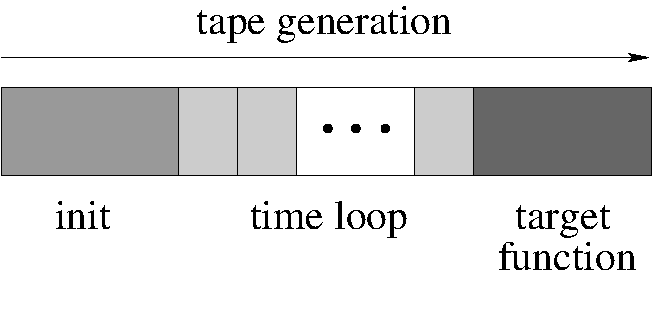
\includegraphics[width=5.8cm]{tapebasic}\hfill
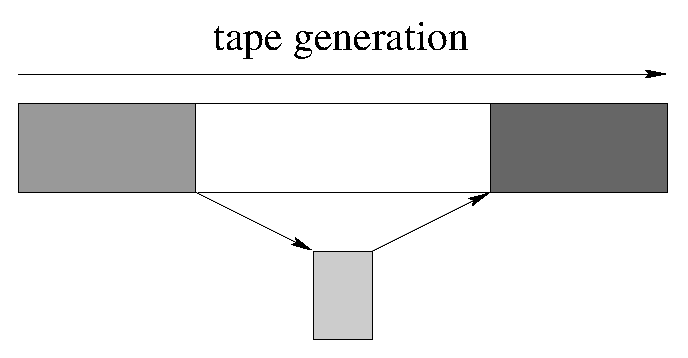
\includegraphics[width=5.8cm]{tapeadv} \hspace*{0.5cm}\ 
\end{center}
\hspace*{0.8cm} Basic taping process \hspace*{4.3cm} Advanced taping process
\caption{Different taping approaches}
\label{fig:bas_tap}
\end{figure} 
As can be seen, the iterative process is completely
unrolled due to the taping process. That is, the tape contains an internal representation of each 
time step. Hence, the overall tape comprises a serious amount of redundant
information as illustrated by the light grey rectangles in
\autoref{fig:bas_tap}.  

To overcome the repeated storage of essentially the same information, 
a {\em nested taping} mechanism has been incorporated into ADOL-C as illustrated on
the right-hand side of \autoref{fig:bas_tap}. This new
capability allows the encapsulation of the time-stepping procedure
such that only the last time step $x_{N} = F(x_{N-1},u_{N-1})$ is taped as one
representative of the time steps in addition to a function pointer to the 
evaluation procedure $F$ of the time steps.  The function pointer has
to be stored for a possibly necessary retaping during the derivative calculation
as explained below. 

Instead of storing the complete tape, only a very limited number of intermediate
states are kept in memory. They serve as checkpoints, such that
the required information for the backward integration is generated
piecewise during the adjoint calculation.
For this modified adjoint computation the optimal checkpointing schedules
provided by {\bf revolve} are employed. An adapted version of the
software package {\sf revolve} is part of ADOL-C and automatically
integrated in the ADOL-C library. Based on {\sf revolve}, $c$ checkpoints are
distributed such that computational effort is minimized for the given
number of checkpoints and time steps $N$. It is important to note that the overall tape
size is drastically reduced due to the advanced taping strategy.  For the
implementation of this nested taping we introduced 
a so-called ``differentiating context'' that enables \mbox{ADOL-C} to
handle different internal function representations during the taping 
procedure and the derivative calculation. This approach allows the generation of a new
tape inside the overall tape, where the coupling of the different tapes is based on
the {\em external differentiated function} described above.

Written under the objective of minimal user effort, the checkpointing routines
of \mbox{ADOL-C} need only very limited information. The user must
provide two routines as implementation of the time-stepping function $F$ 
with the signatures
\medskip

\noindent
\hspace*{2cm}{\sf int time\_step\_function(int n, adouble *u);}\\
\hspace*{2cm}{\sf int time\_step\_function(int n, double *u);}
\medskip

\noindent
where the function names can be chosen by the user as long as the names are
unique.It is possible that the result vector of one time step
iteration overwrites the argument vector of the same time step. Then, no
copy operations are required to prepare the next time step.

At first, the {\sf adouble} version of the time step function has to
be {\em registered} using the \mbox{ADOL-C} function
\medskip

\noindent
\hspace*{2cm}{\sf CP\_Context cpc(time\_step\_function);}.
\medskip

\noindent
This function initializes the structure {\sf cpc}. Then, 
the user has to provide the remaining checkpointing information
by the following commands:
\begin{tabbing}
\hspace*{2cm}\= {\sf cpc.setDoubleFct(time\_step\_function);}\\
             \> {\sf // double variante of the time step function}\\
             \> {\sf cpc.setNumberOfSteps(N);}\\
             \> {\sf // number of time steps to perform}\\
             \> {\sf cpc.setNumberOfCheckpoints(10);}\\
             \> {\sf // number of checkpoint} \\
             \> {\sf cpc.setDimensionXY(n);}\\
             \> {\sf // dimension of input/output}\\
             \> {\sf cpc.setInput(y);}\\
             \> {\sf // input vector} \\
             \> {\sf cpc.setOutput(y);}\\
             \> {\sf // output vector }\\
             \> {\sf cpc.setTapeNumber(tag\_check);}\\
             \> {\sf // subtape number for checkpointing} \\
             \> {\sf cpc.setAlwaysRetaping(false);}\\
             \> {\sf // always retape or not ?}
\end{tabbing}
Subsequently, the time loop in the function evaluation can be
substituted by a call of the function
\medskip

\noindent
\hspace*{2cm}{\sf int cpc.checkpointing();}
\medskip

\noindent
Then, ADOL-C computes derivative information using the optimal checkpointing
strategy provided by {\sf revolve} internally, i.e., completely hidden from the user.

The presented driver is prototyped in the header file 
\verb=<adolc/checkpointing.h>=. This header
is included by the global header file \verb=<adolc/adolc.h>= automatically. 
An example program \verb=checkpointing.cpp= illustrates the
checkpointing facilities. It can be found in the directory \verb=examples/additional_examples/checkpointing=.
%
%
%
\subsection{Advanced algorithmic differentiation of fixed point iterations}
%
Quite often, the state of the considered system denoted by $x\in\R^n$
depends on some design parameters denoted by $u\in\R^m$. One example for this setting
forms the flow over an aircraft wing. Here, the shape of the wing that
is defined by the design vector $u$  
determines the flow field $x$. The desired quasi-steady state $x_*$
fulfills the fixed point equation
\begin{align}
  \label{eq:fixedpoint}
  x_* = F(x_*,u)
\end{align}
for a given continuously differentiable function 
$F:\R^n\times\R^m\rightarrow\R^n$. A fixed point property of this kind is
also exploited by many other applications.

Assume that one can apply the iteration  
\begin{align}
\label{eq:iteration}
 x_{k+1} = F(x_k,u)
\end{align}
to obtain a linear converging sequence $\{x_k\}$ generated
for any given control $u\in\R^n$. Then the limit point $x_*\in\R^n$ fulfils the fixed
point equation~\eqref{eq:fixedpoint}. Moreover,
suppose that $\|\frac{dF}{dx}(x_*,u)\|<1$ holds for any pair
$(x_*,u)$ satisfying equation \eqref{eq:fixedpoint}.
Hence, there exists a
differentiable function $\phi:\R^m \rightarrow \R^n$,
such that $\phi(u) = F(\phi(u),u)$, where the state 
$\phi(u)$ is a fixed point of $F$ according to a control
$u$. To optimize the system described by the state vector $x=\phi(u)$ with respect to
the design vector $u$, derivatives of $\phi$ with respect
to $u$ are of particular interest.

To exploit the advanced algorithmic differentiation  of such fixed point iterations
ADOL-C provides the special functions {\tt fp\_iteration(...)}.
It has the following interface: 
\begin{tabbing}
\hspace{0.5in}\={\sf short int tag;} \hspace{1.1in}\= \kill    % define tab position
\>{\sf int
  fp\_iteration(}\={\sf sub\_tape\_num,double\_F,adouble\_F,norm,norm\_deriv,eps,eps\_deriv,}\\
\>              \>{\sf N\_max,N\_max\_deriv,x\_0,u,x\_fix,dim\_x,dim\_u)}\\
\hspace{0.5in}\={\sf short int tag;} \hspace{0.9in}\= \kill    % define tab position
\>{\sf short int sub\_tape\_num;}         \> // tape identification for sub\_tape \\
\>{\sf int *double\_F;}         \> // pointer to a function that compute for $x$ and $u$ \\
\>                              \> // the value $y=F(x,u)$ for {\sf double} arguments\\             
\>{\sf int *adouble\_F;}        \> // pointer to a function that compute for $x$ and $u$ \\
\>                              \> // the value $y=F(x,u)$ for {\sf double} arguments\\             
\>{\sf int *norm;}              \> // pointer to a function that computes\\
\>                              \> // the norm of a vector\\
\>{\sf int *norm\_deriv;}       \> // pointer to a function that computes\\
\>                              \> // the norm of a vector\\
\>{\sf double eps;}             \> // termination criterion for fixed point iteration\\
\>{\sf double eps\_deriv;}      \> // termination criterion for adjoint fixed point iteration\\
\>{\sf N\_max;}                 \> // maximal number of itertions for state computation\\
\>{\sf N\_max\_deriv;}          \> // maximal number of itertions for adjoint computation\\
\>{\sf adouble *x\_0;}          \> // inital state of fixed point iteration\\
\>{\sf adouble *u;}             \> // value of $u$\\
\>{\sf adouble *x\_fic;}        \> // final state of fixed point iteration\\
\>{\sf int dim\_x;}             \> // dimension of $x$\\
\>{\sf int dim\_u;}             \> // dimension of $u$\\
\end{tabbing}
%
Here {\tt sub\_tape\_num} is an ADOL-C identifier for the subtape that
should be used for the fixed point iteration.
{\tt double\_F} and {\tt adouble\_F} are pointers to functions, that
compute for $x$ and $u$ a single iteration step $y=F(x,u)$. Thereby
{\tt double\_F} uses {\tt double} arguments and {\tt adouble\_F}
uses ADOL-C {\tt adouble} arguments. The parameters {\tt norm} and
{\tt norm\_deriv} are pointers to functions computing the norm
of a vector. The latter functions together with {\tt eps},
{\tt eps\_deriv}, {\tt N\_max}, and {\tt N\_max\_deriv} control
the iterations. Thus the following loops are performed:
\begin{center}
\begin{tabular}{ll}
  do                     &   do                           \\
  ~~~~$k = k+1$          &   ~~~~$k = k+1$                \\
  ~~~~$x = y$            &   ~~~~$\zeta = \xi$            \\
  ~~~~$y = F(x,u)$       &   ~~~
  $(\xi^T,\bar u^T) = \zeta^TF'(x_*,u) + (\bar x^T, 0^T)$ \\
  while $\|y-x\|\geq\varepsilon$ and $k\leq N_{max}$ \hspace*{0.5cm} &
  while $\|\xi -\zeta\|_{deriv}\geq\varepsilon_{deriv}$   \\
  & and $k\leq N_{max,deriv}$
\end{tabular}
\end{center}
The vector for the initial iterate and the control is stored
in {\tt x\_0} and {\tt u} respectively. The vector in which the
fixed point is stored is {\tt x\_fix}. Finally {\tt dim\_x}
and {\tt dim\_u} represent the dimensions $n$ and $m$ of the
corresponding vectors.

The presented driver is prototyped in the header file 
\verb=<adolc/fixpoint.h>=. This header
is included by the global header file \verb=<adolc/adolc.h>= automatically. 
An example code that shows also the
expected signature of the function pointers is contained in the directory \verb=examples/additional_examples/fixpoint_exam=.
%
\subsection{Advanced algorithmic differentiation of OpenMP parallel programs}
%
ADOL-C allows to compute derivatives in parallel for functions
containing OpenMP parallel loops.
This implies that an explicit loop-handling approach is applied. A
typical situation is shown in \autoref{fig:basic_layout},
\begin{figure}[hbt]
    \vspace{3ex}
    \begin{center}
        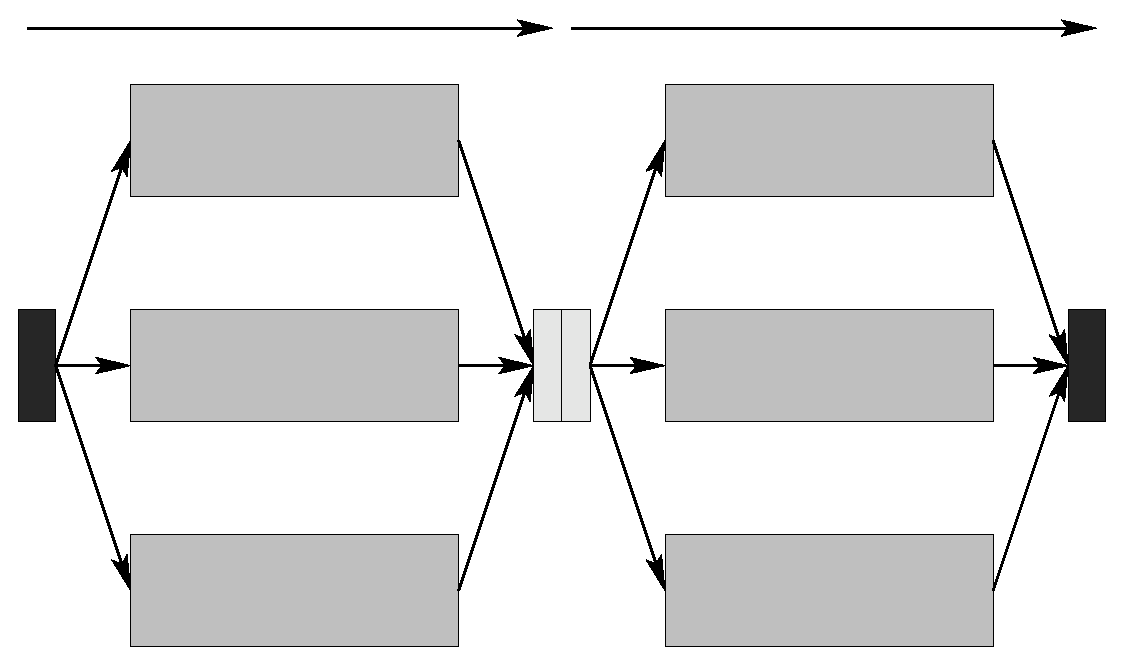
\includegraphics[height=4cm]{multiplexed} \\
        \begin{picture}(0,0)
            \put(-48,40){\vdots}
            \put(48,40){\vdots}
            \put(-48,80){\vdots}
            \put(48,80){\vdots}
            \put(-83,132){function eval.}
            \put(5,132){derivative calcul.}
        \end{picture}
    \end{center}
    \vspace{-5ex}
    \caption{Basic layout of mixed function and the corresponding derivation process}
    \label{fig:basic_layout}
\end{figure}
where the OpenMP-parallel loop is preceded by a serial startup
calculation and followed by a serial finalization phase. 

Initialization of the OpenMP-parallel regions for \mbox{ADOL-C} is only a matter of adding a macro to the outermost OpenMP statement.
Two macros are available that only differ in the way the global tape information is handled.
Using {\tt ADOLC\_OPENMP}, this information, including the values of the augmented variables, is always transferred from the serial to the parallel region using {\it firstprivate} directives for initialization.
For the special case of iterative codes where parallel regions, working on the same data structures, are called repeatedly the {\tt ADOLC\_OPENMP\_NC} macro can be used.
Then, the information transfer is performed only once within the iterative process upon encounter of the first parallel region through use of the {\it threadprivate} feature of OpenMP that makes use of thread-local storage, i.e., global memory local to a thread.
Due to the inserted macro, the OpenMP statement has the following structure:
\begin{tabbing}
\hspace*{1cm} \= {\sf \#pragma omp ... ADOLC\_OPENMP} \qquad \qquad or \\
              \> {\sf \#pragma omp ... ADOLC\_OPENMP\_NC}
\end{tabbing}
Inside the parallel region, separate tapes may then be created.
Each single thread works in its own dedicated AD-environment, and all
serial facilities of \mbox{ADOL-C} are applicable as usual. The global
derivatives can be computed using the tapes created in the serial and
parallel parts of the function evaluation, where user interaction is
required for the correct derivative concatenation of the various tapes.

For the usage of the parallel facilities, the \verb=configure=-command
has to be used with the option \verb?--with-openmp-flag=FLAG?, where 
\verb=FLAG= stands for the system dependent OpenMP flag.
The parallel differentiation of a parallel program is illustrated
by the example program \verb=openmp_exam.cpp= contained in \verb=examples/additional_examples/openmp_exam=.
%
%++++++++++++++++++++++++++++++++++++++++++++++++++++++++++++++++
%
\section{Traceless forward differentiation in ADOL-C}
\label{traceless}
%
Up to version 1.9.0, the development of the ADOL-C software package
was based on the decision to store all data necessary for derivative
computation on traces (tapes), where large applications require the traces to be
written out to corresponding files. In almost all cases this means
a considerable drawback in terms of run time due to the excessive
memory accesses. Using these traces enables ADOL-C to offer multiple
functions. However, it is not necessary for all tasks of derivative
computation to do that. 

Starting with version 1.10.0, ADOL-C now features a traceless forward
mode for computing first order derivatives in scalar mode, i.e.,
$\dot{y} = F'(x)\dot{x}$, and in vector mode, i.e., $\dot{Y} = F'(x)\dot{X}$. 
This traceless variant coexists with the more universal
trace based mode in the package. The following subsections describe
the source code modifications required to use the traceless forward mode of
ADOL-C.  
%
\subsection{Modifying the Source Code}
%
Let us consider the coordinate transformation from Cartesian to spherical
polar coordinates given by the function $F: \mathbb{R}^3 \to \mathbb{R}^3$, $y
= F(x)$, with
\begin{eqnarray*}
y_1  =  \sqrt{x_1^2 + x_2^2 + x_3^2},\qquad
y_2  =  \arctan\left(\sqrt{x_1^2 + x_2^2}/x_3\right),\qquad
y_3  =  \arctan(x_2/x_1),
\end{eqnarray*}
as an example. The corresponding source code is shown in \autoref{fig:traceless}.
\begin{figure}[htb]
\framebox[\textwidth]{\parbox{\textwidth}{
%\begin{center}
%\begin{flushleft}
\begin{tabbing}
\= \kill
\> {\sf \#include} {\sf $<$iostream$>$}\\
\> {\sf using namespace std;}\\
\> \\
\> {\sf int main() \{}\\
\> {\sf \rule{0.5cm}{0pt}double x[3], y[3];}\\
\> \\
\> {\sf \rule{0.5cm}{0pt}for (int i=0; i$<$3; ++i)\hspace*{3cm}// Initialize $x_i$}\\
\> {\sf \rule{1cm}{0pt}...}\\
\> \\
\> {\sf \rule{0.5cm}{0pt}y[0] = sqrt(x[0]*x[0]+x[1]*x[1]+x[2]*x[2]);}\\
\> {\sf \rule{0.5cm}{0pt}y[1] = atan(sqrt(x[0]*x[0]+x[1]*x[1])/x[2]);}\\
\> {\sf \rule{0.5cm}{0pt}y[2] = atan(x[1]/x[0]);}\\
\> \\
\> {\sf \rule{0.5cm}{0pt}cout $<<$ "y1=" $<<$ y[0] $<<$ " , y2=" $<<$ y[1] $<<$ " , y3=" $<<$ y[2] $<<$ endl;}\\
\> \\
\> {\sf \rule{0.5cm}{0pt}return 0;}\\
\> \}
\end{tabbing}
%\end{flushleft}
%\end{center}
}}
\caption{Example for traceless forward mode}
\label{fig:traceless}
\end{figure}
%
Changes to the source code that are necessary for applying the
traceless forward mode of ADOL-C are described in the following two
subsections, where the vector mode version is described
as extension of the scalar mode. 
%
\subsubsection*{The scalar mode}
%
To use the traceless forward mode, one has to include only
the header file \verb#adtl.h# since it does not include the
trace based functions defined in other header files. 

As in the trace based forward version of ADOL-C all derivative
calculations are introduced by calls to overloaded
operators. Therefore, similar to the trace-based version all
independent, intermediate and dependent variables must be declared 
with type {\sf adouble}. The whole traceless functionality provided by
\verb#adtl.h# was written as complete inline intended code
due to run time aspects, where the real portion of inlined code can
be influenced by switches for many compilers. Likely, the whole
derivative code is inlined by default. Our experiments
with the traceless mode have produced complete inlined code by using
standard switches (optimization) for GNU and Intel C++
compiler.

To avoid name conflicts
resulting from the inlining the traceless version has its own namespace
\verb#adtl#. As a result four possibilities of using the {\sf adouble}
type are available for the traceless version: 
\begin{itemize}
\item Defining a new type
      \begin{center}
	\begin{tabular}{l}
	  {\sf typedef adtl::adouble adouble;}\\
	  ...\\
	  {\sf adouble tmp;}
	\end{tabular}
      \end{center}
      This is the preferred way. Remember, you can not write an own
      {\sf adouble} type/class with different meaning after doing the typedef.
\item Declaring with namespace prefix
      \begin{center}
	\begin{tabular}{l}
	  {\sf adtl::adouble tmp;}
	\end{tabular}
      \end{center}
      Not the most handsome and efficient way with respect to coding
      but without any doubt one of the safest ways. The identifier
      {\sf adouble} is still available for user types/classes. 
\item Trusting macros
      \begin{center}
	\begin{tabular}{l}
	  {\sf \#define adouble adtl::adouble}\\
	  ...\\
	  {\sf adouble tmp;}
	\end{tabular}
      \end{center}
      This approach should be used with care, since standard defines are text replacements. 
  \item Using the complete namespace
        \begin{center}
	  \begin{tabular}{l}
	    {\sf using namespace adtl;}\\
	    ...\\
	    {\sf adouble tmp;}
	  \end{tabular}
	\end{center}
	A very clear approach with the disadvantage of uncovering all the hidden secrets. Name conflicts may arise!
\end{itemize}
After defining the variables only two things are left to do. First 
one needs to initialize the values of the independent variables for the
function evaluation. This can be done by assigning the variables a {\sf
double} value. The {\sf ad}-value is set to zero in this case. 
Additionally, the traceless forward mode variant of ADOL-C
offers a function named {\sf setValue} for setting the value without
changing the {\sf ad}-value. To set the {\sf ad}-values of the independent
variables ADOL-C offers two possibilities:
\begin{itemize}
  \item Using the constructor
        \begin{center}
	  \begin{tabular}{l}
        {\sf double seedOne = 1., seedZero = 0.;}\\
	    {\sf adouble x1(2,\&seedOne), x2(4,\&seedZero), y;}
	  \end{tabular}
	\end{center}
	This would create three adoubles $x_1$, $x_2$ and $y$. Obviously, the latter
	remains uninitialized. In terms of function evaluation
	$x_1$ holds the value 2 and $x_2$ the value 4 whereas the derivative values
	are initialized to $\dot{x}_1=1$ and $\dot{x}_2=0$.
   \item Setting point values directly
         \begin{center}
	   \begin{tabular}{l}
         {\sf double seedOne = 1., seedZero = 0.;}\\
	     {\sf adouble x1=2, x2=4, y;}\\
	     ...\\
	     {\sf x1.setADValue(\&seedOne);}\\
	     {\sf x2.setADValue(\&seedZero);}
	   \end{tabular}
	 \end{center}
	 The same example as above but now using {\sf setADValue}-method for initializing the derivative values. It is important to note that in both cases the derivative values have to be set by passing an address of a variable or a pointer of the {\sf double} type (instead of passing the value directly). The reason for doing this will become clear in the next subsection. 
\end{itemize}
%
The derivatives can be obtained at any time during the evaluation
process by calling the {\sf getADValue}-method which returns a pointer (instead of a value), and therefore, it can be assigned to another pointer or it can be dereferenced immediately in order to read the value:
\begin{center}
  \begin{tabular}{l}
    {\sf adouble y;}\\
    ...\\
    {\sf cout $<<$ *(y.getADValue());}
  \end{tabular}
\end{center}
\autoref{fig:modcode} shows the resulting source code incorporating
all required changes for the example
given above.

\begin{figure}[htb]
\framebox[\textwidth]{\parbox{\textwidth}{
%\begin{center}
\begin{tabbing}
\hspace*{-1cm} \= \kill
\> {\sf \#include $<$iostream$>$}\\
\> {\sf using namespace std;}\\
\> \\
\> {\sf \#include $<$adolc/adtl.h$>$}\\
\> {\sf typedef adtl::adouble adouble;}\\
\\
\> {\sf int main() \{}\\
\> {\sf \rule{0.5cm}{0pt}adouble x[3], y[3];}\\
\\
\> {\sf \rule{0.5cm}{0pt}for (int i=0; i$<$3; ++i)\hspace*{3cm}// Initialize $x_i$}\\
\> {\sf \rule{1cm}{0pt}...}\\
\\
\> {\sf \rule{0.5cm}{0pt}double seed = 1.;}\\
\> {\sf \rule{0.5cm}{0pt}x[0].setADValue(\&seed);\hspace*{3cm}// derivative of f with respect to $x_1$}\\
\> {\sf \rule{0.5cm}{0pt}y[0] = sqrt(x[0]*x[0]+x[1]*x[1]+x[2]*x[2]);}\\
\> {\sf \rule{0.5cm}{0pt}y[1] = atan(sqrt(x[0]*x[0]+x[1]*x[1])/x[2]);}\\
\> {\sf \rule{0.5cm}{0pt}y[2] = atan(x[1]/x[0]);}\\
\\
\> {\sf \rule{0.5cm}{0pt}cout $<<$ "y1=" $<<$ y[0].getValue() $<<$ " , y2=" $<<$ y[1].getValue ... ;}\\
\> {\sf \rule{0.5cm}{0pt}cout $<<$ "dy2/dx1 = " $<<$ *(y[1].getADValue()) $<<$ endl;}\\
\> {\sf \rule{0.5cm}{0pt}return 0;}\\
\> {\sf \}}
\end{tabbing}
%\end{center}
}}
\caption{Example for traceless scalar forward mode}
\label{fig:modcode}
\end{figure}
%
\subsubsection*{The vector mode}
%
In scalar mode only one direction element has to be stored per {\sf
  adouble} whereas a field of $p$ elements is needed in the vector
  mode to cover the computations for the given $p$ directions. The
  resulting changes to the source code are described in this section. 

In order to use the vector mode one has to call
\verb#adtl::setNumDir(N)#.  This function takes the maximal number of
directions to be used within the resulting vector mode. Changing the
number of directions in the middle of executing code containing active
variables is undesirable and can lead to segmentation violations,
hence such an operation will result in an
error. \verb#adtl::setNumDir(N)# must therefore be called before
declaring any \verb#adtl::adouble# objects.

Setting and getting the derivative values is done in the same manner as in the scalar case, by passing and retrieving the pointers, as illustrated in the following example:
\begin{center}
  \begin{tabular}{l}
    {\sf adtl::setNumDir(10);}\\
    {\sf adouble x, y;}\\
    {\sf double *ptr1 = new double[10];}\\
    {\sf double *ptr2;}\\
      ...\\
    {\sf x1=2;}\\
    {\sf x1.setADValue(ptr1);}\\
    ...\\
    {\sf ptr2=y.getADValue();}
  \end{tabular}
\end{center}
Now using the pointers in the methods {\sf setADValue} and {\sf getADValue} makes more sense since the vector mode requires the field of $p$ elements per {\sf adouble} which holds the derivative values.
Additionally, the traceless vector forward mode of ADOL-C offers two
new methods for setting/getting the derivative values. Setting a derivative value of the desired vector element is possible by passing a {\sf double} value and its position in the vector ({\sf integer}). Getting a derivative value of the desired vector element requires as argument only its position in the vector. One can note that the pointers are not used in these cases, as illustrated in the following example:
\begin{center}
  \begin{tabular}{l}
    {\sf adtl::setNumDir(10);}\\
    ...\\
    {\sf adouble x, y;}\\
    ...\\
    {\sf x1=2;}\\
    {\sf x1.setADValue(5,1);\hspace*{3.7cm}// set the 6th point value of x to 1.0}\\
      ...\\
    {\sf cout $<<$ y.getADValue(3) $<<$ endl;\hspace*{1cm}// print the 4th derivative value of y}
  \end{tabular}
\end{center}
The resulting source code containing all changes that are required is
shown in \autoref{fig:modcode2}

\begin{figure}[!h!t!b]
\framebox[\textwidth]{\parbox{\textwidth}{
\begin{tabbing}
\hspace*{-1cm} \= \kill
\> {\sf \#include $<$iostream$>$}\\
\> {\sf  using namespace std;}\\
\\
\> {\sf \#include $<$adolc/adtl.h$>$}\\
\> {\sf typedef adtl::adouble adouble;}\\
\\
\> {\sf int main() \{}\\
\> {\sf \rule{0.5cm}{0pt}adtl::setNumDir(3);}\\
\> {\sf \rule{0.5cm}{0pt}adouble x[3], y[3];}\\
\\
\> {\sf \rule{0.5cm}{0pt}for (int i=0; i$<$3; ++i) \{}\\
\> {\sf \rule{1cm}{0pt}...\hspace*{3cm}// Initialize $x_i$}\\
\> {\sf \rule{1cm}{0pt}for (int j=0; j$<$3; ++j) if (i==j) x[i].setADValue(j,1);}\\
\> {\sf \rule{0.5cm}{0pt}\}}\\
\\
\> {\sf \rule{0.5cm}{0pt}y[0] = sqrt(x[0]*x[0]+x[1]*x[1]+x[2]*x[2]);}\\
\> {\sf \rule{0.5cm}{0pt}y[1] = atan(sqrt(x[0]*x[0]+x[1]*x[1])/x[2]);}\\
\> {\sf \rule{0.5cm}{0pt}y[2] = atan(x[1]/x[0]);}\\
\\
\> {\sf \rule{0.5cm}{0pt}cout $<<$ "y1=" $<<$ y[0].getValue() $<<$ " , y2=" $<<$ y[1].getValue ... ;}\\
\> {\sf \rule{0.5cm}{0pt}cout $<<$ "jacobian : " $<<$ endl;}\\
\> {\sf \rule{0.5cm}{0pt}for (int i=0; i$<$3; ++i) \{}\\
\> {\sf \rule{1cm}{0pt}for (int j=0; j$<$3; ++j)}\\
\> {\sf \rule{1.5cm}{0pt}cout $<<$ y[i].getADValue(j) $<<$ "  ";}\\
\> {\sf \rule{1cm}{0pt}cout $<<$ endl;}\\
\> {\sf \rule{0.5cm}{0pt}\}}\\
\> {\sf \rule{0.5cm}{0pt}return 0;}\\
\> {\sf \}}
\end{tabbing}
}}
\caption{Example for traceless vector forward mode}
\label{fig:modcode2}
\end{figure}
%
\subsection{Compiling and Linking the Source Code}
%
After incorporating the required changes, one has to compile the
source code and link the object files to get the executable. 
As long as the ADOL-C header files are not included in the absolute path
the compile sequence should be similar to the following example:
\begin{center}
  \begin{tabular}{l}
    {\sf g++ -I/home/username/adolc\_base/include -c traceless\_scalar.cpp}
  \end{tabular}
\end{center}
The \verb#-I# option tells the compiler where to search for the ADOL-C
header files. This option can be omitted when the headers are included
with absolute path or if ADOL-C is installed in a ``global'' directory. 

Although originally designed to be completely inline, certain global
variables need to be initialised in the compiled part of the library
and therefore the ADOL-C library must be linked with the compiled code.
The example started above could be finished with the
following command:
\begin{center}
  \begin{tabular}{l}
    {\sf g++ -o traceless\_scalar traceless\_scalar.o}\\
    {\sf -Wl,-{}-rpath -Wl,/home/username/adolc\_base/lib -L/home/username/adolc\_base/lib -ladolc}
  \end{tabular}
\end{center}
The mentioned source codes {\sf traceless\_scalar.c} and {\sf traceless\_vector.c} 
illustrating the use of the for traceless scalar and vector mode can be found in
the directory {\sf examples}. 
%
\subsection{Concluding Remarks for the Traceless Forward Mode Variant}
%
As many other AD methods the traceless forward mode provided by the
ADOL-C package has its own strengths and drawbacks. Please read the
following section carefully to become familiar with the things that
can occur: 
\begin{itemize}
  \item Advantages:
    \begin{itemize}
      \item Code speed\\
	Increasing computation speed was one of the main aspects in writing
	the traceless code. In many cases higher performance can be
	expected this way. However this is not guarenteed for repeated
        evaluations.
      \item Smaller overall memory requirements\\
	Traceless ADOL-C does not write traces anymore, as the name
	implies. Loop ''unrolling'' can be avoided this
	way. Considered main memory plus disk space as overall memory
	requirements the traceless version can be 
	executed in a more efficient way. 
    \end{itemize}
  \item Drawbacks:
    \begin{itemize}
    \item Main memory limitations\\
      The ability to compute derivatives to a given function is
      bounded by the main memory plus swap size  when using
      traceless ADOL-C. Computation from swap should be avoided anyway
      as far as possible since it slows down the computing time
      drastically. Therefore, if the program execution is  
      terminated without error message insufficient memory size can be
      the reason among other things. The memory requirements $M$ can
      be determined roughly as followed: 
      \begin{itemize}
        \item Scalar mode: $M=$(number of {\sf adouble}s)$*2 + M_p$
	\item Vector mode: $M=$(number of {\sf adouble}s)*({\sf
	  NUMBER\_DIRECTIONS}$+1) + M_p$ 
      \end{itemize}
      where the storage size of all non {\sf adouble} based variables is described by $M_p$.
    \item Compile time\\
      As discussed in the previous sections, the traceless forward mode of
      the ADOL-C package is implemented as inline intended version. Using
      this approach results in a higher source code size, since every
      operation involving at least one {\sf adouble} stands for the
      operation itself as well as for the corresponding derivative
      code after the inlining process. Therefore, the compilation time
      needed for the traceless version may be higher than that of the trace based code. 
    \item Code Size\\
      A second drawback and result of the code inlining is the
      increase of code sizes for the binaries. The increase
      factor compared to the corresponding trace based program is
      difficult to quantify as it is task dependent. Practical results
      have shown that values between 1.0 and 2.0 can be
      expected. Factors higher than 2.0 are possible too and even
      values below 1.0 have been observed. 
    \end{itemize}
\end{itemize}


\section{Traceless forward differentiation in ADOL-C using Cuda}
\label{tracelessCuda}
%
One major drawback using the traceless version of ADOL-C is the fact 
that several function evaluations are needed to compute derivatives
in many different points. More precisely, to calculate the Jacobian for
a function $F:\mathbb{R}^n\rightarrow \mathbb{R}^m$ in $M$ points, $M$
function evaluations are needed for the traceless vector mode and even 
$M*n$ for the traceless scalar mode. Depending on the size of the function 
this can result in a long runtime. To achieve a better performance one can
use parallelisation techniques as the same operations are
performed during a function evaluation. One possibility is to use GPUs 
since they are optimized for data parallel computation. Starting with 
version 2.3.0 ADOL-C now features a traceless forward mode for computing 
first order derivatives in scalar mode on GPUs using the 
general purpose parallel computing architecture Cuda. 

The idea is to include parallel code that executes in many GPU threads across
processing elements. This can be done by using kernel functions, that is functions
which are executed on GPU as an array of threads in parallel. In general all 
threads execute the same code. They are grouped into blocks which are then grouped 
into grids. A kernel is executed as a grid of blocks of threads. For more 
details see, e.g., the NVIDIA CUDA C Programming Guide which can be downloaded from 
the web page {\sf www.nvidia.com}. To solve the problem of calculating 
the Jacobian of $F$ at $M$ points it is possible to let each thread perform a 
function evaluation and thus the computation of derivatives for one direction 
at one point. The advantage is that the function is evaluated in different points
in parallel which can result in a faster wallclock runtime.

The following subsection describes the source code modifications required to use 
the traceless forward mode of ADOL-C with Cuda.  

\subsection{Modifying the source code}

Let us again consider the coordinate transformation from Cartesian to spherical
polar coordinates given by the function $F: \mathbb{R}^3 \to \mathbb{R}^3$, $y
= F(x)$, with
\begin{eqnarray*}
y_1  =  \sqrt{x_1^2 + x_2^2 + x_3^2},\qquad
y_2  =  \arctan\left(\sqrt{x_1^2 + x_2^2}/x_3\right),\qquad
y_3  =  \arctan(x_2/x_1),
\end{eqnarray*}
as an example. We now calculate the Jacobian at $M=1024$ different points.
The source code for one point is shown in \autoref{fig:traceless}. This example 
has no real application but can still be used to show the combination of the traceless version
of ADOL-C and Cuda.

For the use of this mode a Cuda toolkit, which is suitable for the grafic card used,
has to be installed. Furthermore, it is important to check that the graphic card
used supports double precision (for details see e.g. NVIDIA CUDA C Programming Guide).
Otherwise the data type employed inside of the {\sf adouble} class has to be adapted
to {\sf float}. To use the traceless forward mode with Cuda, one has to include the header
files \verb#adoublecuda.h# and \verb#cuda.h#. The first one contains the 
definition of the class {\sf adouble} and the overloaded operators
for this version of ADOL-C. As in the other versions all derivative 
calculations are introduced by calls to overloaded operators. The 
second header file is needed for the use of Cuda.  

One possibility to solve the problem above is the following. First of all
three {\sf double} arrays are needed: {\sf x} for the independent variables, 
{\sf y} for the dependent variables and {\sf deriv} for the values of the 
Jacobian matrices. The independent variables have to be initialised, therefore 
the points at which the function should be evaluated are saved in a row in the 
same array of length $3*M$. For the computation on GPUs one also has to allocate memory
on this device. Using the syntax in Cuda one can allocate an array of 
length $3*M$ (number of independent variables times number of points) for 
the independent variables as follows:
\begin{center}
  \begin{tabular}{l}
    {\sf double * devx;}\\
    {\sf cudaMalloc((void**)\&devx, 3*M*sizeof(double));}\\
  \end{tabular}
\end{center}
The arrays for the dependent variables and the values of the Jacobian matrices
are allocated in the same way. Then the values of the independent variables 
have to be copied to the GPU using the following command
\begin{center}
  \begin{tabular}{l}
    {\sf cudaMemcpy(devx, x, sizeof(double)*3*M, cudaMemcpyHostToDevice);}\\
  \end{tabular}
\end{center}   
The argument {\sf cudaMemcpyHostToDevice} indicates that the values are copied from 
the host to the GPU. In this case the values stored in {\sf x} are copied to {\sf devx}. 

Now all required information has been transferred to the GPU. The changes 
in the source code made so far are summarized in \autoref{fig:cudacode1}.
 
\begin{figure}[!h!t!b]
\framebox[\textwidth]{\parbox{\textwidth}{
%\begin{center}
\begin{tabbing}
\hspace*{-1cm} \= \kill
\> {\sf \#include $<$iostream$>$}\\
\> {\sf \#include $<$cuda.h$>$}\\
\> {\sf \#include $<$adoublecuda.h$>$}\\
\> {\sf using namespace std;}\\
\\
\> {\sf int main() \{}\\
\> {\sf \rule{0.5cm}{0pt}int M=1024;}\\
\> {\sf \rule{0.5cm}{0pt}double* deriv = new double[9*M];}\\
\> {\sf \rule{0.5cm}{0pt}double* y = new double[3*M];}\\
\> {\sf \rule{0.5cm}{0pt}double* x = new double[3*M];}\\
\\
\> {\sf \rule{0.5cm}{0pt}// Initialize $x_i$}\\
\> {\sf \rule{0.5cm}{0pt}for (int k=0; k$<$M; ++k)\{}\\
\> {\sf \rule{1cm}{0pt}for (int i=0; i$<$3; ++i)}\\
\> {\sf \rule{1.5cm}{0pt}x[k*3+i] =i + 1/(k+1);\}}\\
\\
\> {\sf \rule{0.5cm}{0pt}// Allocate array for independent and dependent variables}\\
\> {\sf \rule{0.5cm}{0pt}// and Jacobian matrices on GPU}\\
\> {\sf \rule{0.5cm}{0pt}double * devx;}\\
\> {\sf \rule{0.5cm}{0pt}cudaMalloc((void**)\&devx, 3*M*sizeof(double));}\\
\> {\sf \rule{0.5cm}{0pt}double * devy;}\\
\> {\sf \rule{0.5cm}{0pt}cudaMalloc((void**)\&devy, 3*M*sizeof(double));}\\
\> {\sf \rule{0.5cm}{0pt}double * devderiv;}\\
\> {\sf \rule{0.5cm}{0pt}cudaMalloc((void**)\&devderiv, 3*3*M*sizeof(double));}\\
\\
\> {\sf \rule{0.5cm}{0pt}// Copy values of independent variables from host to GPU}\\
\> {\sf \rule{0.5cm}{0pt}cudaMemcpy(devx, x, sizeof(double)*3*M, cudaMemcpyHostToDevice);}\\
\\
\> {\sf \rule{0.5cm}{0pt}// Call function to specify amount of blocks and threads to be used}\\
\> {\sf \rule{0.5cm}{0pt}kernellaunch(devx, devy, devderiv,M);}\\
\\
\> {\sf \rule{0.5cm}{0pt}// Copy values of dependent variables and Jacobian matrices from GPU to host}\\
\> {\sf \rule{0.5cm}{0pt}cudaMemcpy(y, devy, sizeof(double)*3*M,cudaMemcpyDeviceToHost);}\\
\> {\sf \rule{0.5cm}{0pt}cudaMemcpy(deriv, devderiv, sizeof(double)*3*3*M, cudaMemcpyDeviceToHost);}\\
\> {\sf \}}
\end{tabbing}
%\end{center}
}}
\caption{Example for traceless scalar forward mode with Cuda}
\label{fig:cudacode1}
\end{figure}

In the next step the user has to specify how many blocks and threads per block
will be needed for the function evaluations. In the present example this is done by  
the call of the function {\sf kernellaunch}, see \autoref{fig:cudacode2}.
In this case the blocks are two dimensional: the x-dimension is determined
by the number of points $M$ at which the Jacobian matrix has to be calculated 
while the y-dimension is given by the number of independent variables, i.e., 3.
Since a block cannot contain more than 1024 threads, the
x-dimension in the example is 64 instead of $M=1024$. Therefore $1024/64=16$
blocks are needed. The described division into blocks is reasonable as each 
thread has to perform a function evaluation for one point and one direction,
hence $M*3$ threads are needed where 3 denotes the number of independent 
variables corresponding to the number of directions needed for the computation 
of the Jacobian in one point. 

\begin{figure}[!h!t!b]
\framebox[\textwidth]{\parbox{\textwidth}{
\begin{tabbing}
\hspace*{-1cm} \= \kill
\> {\sf cudaError\_t kernellaunch(double* inx, double* outy, double* outderiv, int M) \{}\\
\> {\sf \rule{0.5cm}{0pt}// Create 16 blocks}\\
\> {\sf \rule{0.5cm}{0pt}int Blocks=16;}\\
\> {\sf \rule{0.5cm}{0pt}// Two dimensional (M/Blocks)$\times$3 blocks}\\
\> {\sf \rule{0.5cm}{0pt}dim3 threadsPerBlock(M/Blocks,3);}\\
\\
\> {\sf \rule{0.5cm}{0pt}// Call kernel function with 16 blocks with (M/Blocks)$\times$3 threads per block}\\
\> {\sf \rule{0.5cm}{0pt}kernel $<<<$ Blocks, threadsPerBlock $>>>$(inx, outy, outderiv);}\\
\> {\sf \rule{0.5cm}{0pt}cudaError\_t cudaErr = cudaGetLastError();}\\
\\
\> {\sf \rule{0.5cm}{0pt}return cudaErr;}\\
\> {\sf \}}
\end{tabbing}
}}
\caption{Example for traceless scalar forward mode with Cuda}
\label{fig:cudacode2}
\end{figure}

We can now perform the function evaluations together with the calculation 
of the Jacobians. The corresponding code is illustrated in \autoref{fig:cudacode3}.
Since the function evaluations should be performed on a GPU a kernel function is
needed which is defined by using the \mbox{{\sf \_\_ global\_\_}} declaration specifier 
(see \autoref{fig:cudacode3}). Then each thread executes the operations that are
defined in the kernel. 

\begin{figure}[!h!t!b]
\framebox[\textwidth]{\parbox{\textwidth}{
\begin{tabbing}
\hspace*{-1cm} \= \kill
\> {\sf \_\_global\_\_ void kernel(double* inx, double* outy, double* outderiv) \{}\\
\> {\sf \rule{0.5cm}{0pt}const int index = threadIdx.x ;}\\
\> {\sf \rule{0.5cm}{0pt}const int index1 = threadIdx.y;}\\
\> {\sf \rule{0.5cm}{0pt}const int index2 = blockIdx.x;}\\
\> {\sf \rule{0.5cm}{0pt}const int index3 = blockDim.x;}\\
\> {\sf \rule{0.5cm}{0pt}const int index4 = blockDim.x*blockDim.y;}\\
\\
\> {\sf \rule{0.5cm}{0pt}// Declare dependent and independent variables as {\sf adouble}s}\\
\> {\sf \rule{0.5cm}{0pt}adtlc::adouble y[3], x[3];}\\
\> {\sf \rule{0.5cm}{0pt}// Read out point for function evaluation}\\
\> {\sf \rule{0.5cm}{0pt}for(int i=0; i $<$ 3; i++)}\\
\> {\sf \rule{1cm}{0pt}x[i]=inx[index2*index4+index*3+i];}\\
\> {\sf \rule{0.5cm}{0pt}// Set direction for calculation of derivatives}\\
\> {\sf \rule{0.5cm}{0pt}x[index1].setADValue(1);}\\
\\
\> {\sf \rule{0.5cm}{0pt}// Function evaluation}\\
\> {\sf \rule{0.5cm}{0pt}y[0] = sqrt(x[0]*x[0]+x[1]*x[1]+x[2]*x[2]);}\\
\> {\sf \rule{0.5cm}{0pt}y[1] = atan(sqrt(x[0]*x[0]+x[1]*x[1])/x[2]);}\\
\> {\sf \rule{0.5cm}{0pt}y[2] = atan(x[1]/x[0]);}\\
\\
\> {\sf \rule{0.5cm}{0pt}for(int i=0; i $<$ 3; i++)}\\
\> {\sf \rule{1cm}{0pt}outy[(index2*index3+index)*3+i]=y[i].getValue();}\\
\> {\sf \rule{0.5cm}{0pt}for(int i=0; i $<$ 3; i++)}\\
\> {\sf \rule{1cm}{0pt}outderiv[(index2*index4+index*3+index1)*3+i]=y[i].getADValue();}\\
\> {\sf \}}
\end{tabbing}
}}
\caption{Example for traceless scalar forward mode with Cuda}
\label{fig:cudacode3}
\end{figure}

In this example each thread is assigned the task of calculating the 
derivatives in one point with respect to one independent variable. Therefore
some indices are needed for the implementation. Each thread has a unique thread
ID in a block consisting of an x and an y-dimension. The blocks have an ID as
well. In the example the following indices are used.
 
\begin{itemize}
 \item {\sf index = threadIdx.x} denotes the x-dimension of a thread (ranges from 0 to 63 in the example)
 \item {\sf index1 = threadIdx.y} denotes the y-dimension of a thread (ranges from 0 to 2 in the example)
 \item {\sf index2 = blockIdx.x} denotes the block index (ranges from 0 to 15 in the example)
 \item {\sf index3 = blockDim.x} denotes the x-dimension of a block (always 64 in the example)
 \item {\sf index4 = blockDim.x*blockDim.y} denotes the size of a block (always $64*3=192$ in the example)
\end{itemize}

For the calculation of derivatives the function evaluation has to be performed
with {\sf adouble}s. Therefore the dependent and the independent variables
have to be declared as {\sf adouble}s as in the other versions of ADOL-C (see, e.g., \autoref{traceless}). 
Similar to the traceless version without Cuda the namespace \verb#adtlc# is used. 
Now each thread has to read out the point at which the function evaluation is 
then performed. This is determined by the blockindex and the x-dimension of 
the thread, therefore the independent variables in a thread
have the values
\begin{center}
  \begin{tabular}{l}
    {\sf \rule{0.5cm}{0pt}x[i]=inx[index2*index4+index*3+i];}\\
  \end{tabular}
\end{center}  
for {\sf i=0,1,2} where {\sf inx} corresponds to the vector {\sf devx}. The direction for 
the derivatives is given by {\sf index1}.
\begin{center}
  \begin{tabular}{l}
     {\sf \rule{0.5cm}{0pt}x[index1].setADValue(1);}\\
  \end{tabular}
\end{center} 
The functions for setting and getting the value and the derivative value of an 
{\sf adouble} are the same as in the traceless version of ADOL-C for first 
order derivatives (see \autoref{traceless}).
The function evaluation is then performed with {\sf adouble x} on GPU and the results
are saved in {\sf adouble y}. The function evaluation itself remains unchanged
(see \autoref{fig:cudacode3}). Then we store the values of the function
evaluations in each point in a row in one array:
\begin{center}
  \begin{tabular}{l}
   {\sf \rule{0.5cm}{0pt}outy[(index2*index3+index)*3+i]=y[i].getValue();}\\
  \end{tabular}
\end{center} 
for {\sf i=0,1,2}. The values of a Jacobian are stored column by column in 
a row:
\begin{center}
  \begin{tabular}{l}
   {\sf \rule{0.5cm}{0pt}outderiv[(index2*index4+index*3+index1)*3+i]=y[i].getADValue();}\\
  \end{tabular}
\end{center} 
for {\sf i=0,1,2}. 

Now there is one thing left to do. The values calculated on the GPU have to be copied 
back to host. For the dependent variables in the example this can be done by the 
following call:
\begin{center}
  \begin{tabular}{l}
 {\sf \rule{0.5cm}{0pt}cudaMemcpy(y, devy, sizeof(double)*3*M,cudaMemcpyDeviceToHost);}\\
  \end{tabular}
\end{center} 
see \autoref{fig:cudacode1}. The argument {\sf cudaMemcpyDeviceToHost} determines that
the values are copied from GPU to host.

%
\subsection{Compiling and Linking the Source Code}
%
After incorporating the required changes, one has to compile the
source code and link the object files to get the executable. For 
the compilation of a Cuda file the {\sf nvcc} compiler is needed.
The compile sequence should be similar to the following example:
\begin{center}
  \begin{tabular}{l}
    {\sf nvcc -arch=sm\_20 -o traceless\_cuda traceless\_cuda.cu}
  \end{tabular}
\end{center}
The compiler option \verb#-arch=sm_20# specifies the compute capability that is 
assumed, in this case one that supports double precision.

The mentioned source code {\sf traceless\_cuda.cu} illustrating the use of the
forward traceless scalar mode with Cuda and a further example {\sf liborgpu.cu}
can be found in the directory examples. The second example is an adaption of
the OpenMP example to the traceless version with Cuda.

%
%++++++++++++++++++++++++++++++++++++++++++++++++++++++++++++++++
\section{Installing and Using ADOL-C}
\label{install}
%
\subsection{Generating the ADOL-C Library}
\label{genlib}
%
The currently built system is best summarized by the ubiquitous gnu
install triplet 
\begin{center}
\verb=configure - make - make install= .
\end{center}
Executing this three steps from the package base directory
\verb=</SOMEPATH/=\texttt{\packagetar}\verb=>= will compile the static and the dynamic
ADOL-C library with default options and install the package (libraries
and headers) into the default installation directory {\tt
  \verb=<=\$HOME/adolc\_base\verb=>=}. Inside the install directory
the subdirectory \verb=include= will contain all the installed header
files that may be included by the user program, the subdirectory
\verb=lib= will contain the 32-bit compiled library 
and the subdirectory \verb=lib64= will contain the 64-bit compiled
library. Depending on the compiler only one of \verb=lib= or
\verb=lib64= may be created.

Before doing so the user may modify the header file \verb=usrparms.h=
in order to tailor the \mbox{ADOL-C} package to the needs in the
particular system environment as discussed in 
\autoref{Customizing}. The configure procedure which creates the necessary
\verb=Makefile=s can be customized by use of some switches. Available
options and their meaning can be obtained by executing
\verb=./configure --help= from the package base directory. 

All object files and other intermediately generated files can be
removed by the call \verb=make clean=. Uninstalling ADOL-C by
executing \verb=make uninstall= is only reasonable after a previous
called \verb=make install= and will remove all installed package files
but will leave the created directories behind. 

The sparse drivers are included in the ADOL-C libraries if the
\verb=./configure= command is executed with the option
\verb=--enable-sparse=. The ColPack library available at 
\verb=http://cscapes.cs.purdue.edu/coloringpage/software.htm= is required to
compute the sparse structures, and is searched for in all the default 
locations. 
In case the library and its headers are installed in a nonstandard path
this may be specified with the \verb?--with-colpack=PATH? option.
It is assumed that the library and its header files have the following
directory structure: \verb?PATH/include? contains all the header
files,
\verb?PATH/lib? contains the 32-bit compiled library and 
\verb?PATH/lib64? contains the 64-bit compiled library. Depending on
the compiler used to compile {\sf ADOL-C} one of these libraries will
be used for linking.
 
The option \verb=--disable-stdczero= turns off the initialization in the {\sf adouble} default 
constructor. This will improve efficiency but requires that there be no implicit array initialization in the code, see 
\autoref{WarSug}.  

Support for MPI and the AdjoinableMPI API (see\\
\verb=http://www.mcs.anl.gov/~utke/AdjoinableMPI/AdjoinableMPIDox/index.html=
) may be enabled using the option \verb=--enable-ampi=. This requires
the presence of MPI compiler wrappers \verb=mpicc= and \verb=mpicxx=
in the \verb=$PATH= and the AdjoinableMPI libraries in the standard
locations. If MPI is installed in a nonstandard path one may specify
this using the \verb?--with-mpi=PATH? option. Similarly if the
AdjoinableMPI libraries are in an nonstandard path this may be
specified using the \verb?--with-ampi=PATH? option.  When MPI and
AdjoinableMPI support is compiled into {\sf ADOL-C} the generated
library will be unsuitable for linking with non-MPI
programs and is called \verb=libadolc_ampi=. Therefore the user
programs should use the flag \verb=-ladolc_ampi= instead of
\verb=-ladolc= in this case. An advanced user may infact specify
whatever name the resulting {\sf ADOL-C} library should have using the
\verb?--with-soname=SONAME? option.


\subsection{Compiling and Linking the Example Programs}
%
The installation procedure described in \autoref{genlib} also
provides the \verb=Makefile=s  to compile the example programs in the
directories \verb=<=\texttt{\packagetar}\verb=>/ADOL-C/examples= and the
additional examples in
\verb=<=\texttt{\packagetar}\verb=>/ADOL-C/examples/additional_examples=. However,
one has to execute the 
\verb=configure= command with  appropriate options for the ADOL-C package to enable the compilation of
examples. Available options are: 
\begin{center}
\begin{tabular}[t]{ll}
\verb=--enable-docexa=&build all examples discussed in this manual\\
&(compare \autoref{example})\\
\verb=--enable-addexa=&build all additional examples\\
&(See file \verb=README= in the various subdirectories)
\end{tabular}
\end{center}

Just calling \verb=make= from the packages base directory generates
all configured examples and the library if necessary. Compiling from
subdirectory \verb=examples= or one of its subfolders is possible
too. At least one kind of the ADOL-C library (static or shared) must
have been built previously in that case. Hence, building the library
is always the first step. 

For Compiling the library and the documented examples on Windows using
Visual Studio please refer to the \verb=<Readme_VC++.txt>= files in 
the \verb=<windows/>=, \verb=<ThirdParty/ColPack/>= and 
\verb=<ADOL-C/examples/>= subdirectories.
%
\subsection{Description of Important Header Files}
\label{ssec:DesIH}
%
The application of the facilities of ADOL-C requires the user 
source code (program or module) to include appropriate 
header files where the desired data types and routines are 
prototyped. The new hierarchy of header files enables the user
to take one of two possible ways to access the right interfaces.
The first and easy way is recommended to beginners: As indicated in
\autoref{globalHeaders} the provided {\em global} header file 
\verb=<adolc/adolc.h>= can be included by any user code to support all
capabilities of ADOL-C depending on the particular programming language
of the source.    

\begin{table}[h]
\center \small
\begin{tabular}{|p{3.6cm}|p{10.5cm}|}\hline
\verb=<adolc/adolc.h>= & 
\begin{tabular*}{10.5cm}{cp{9.5cm}}
  \boldmath $\rightarrow$ \unboldmath
                 & global header file available for easy use of ADOL-C; \\
  $\bullet$      & includes all ADOL-C header files depending on
                   whether the users source is C++ or C code.
\end{tabular*}
\\ \hline
\verb=<adolc/internal/usrparms.h>= &
\begin{tabular*}{10.5cm}{cp{9.5cm}}
  \boldmath $\rightarrow$ \unboldmath
                 & user customization of ADOL-C package (see
                   \autoref{Customizing}); \\
  $\bullet$      & after a change of
                   user options the ADOL-C library \verb=libadolc.*=
                   has to be rebuilt (see \autoref{genlib}); \\
  $\bullet$      & is included by all ADOL-C header files and thus by all user
                   programs.
\end{tabular*} \\ \hline
\end{tabular}
\caption{Global header files}
\label{globalHeaders}
\end{table}  

The second way is meant for the more advanced ADOL-C user: Some source code
includes only those interfaces used by the particular application. 
The respectively needed header files are indicated
throughout the manual.
Existing application determined dependences between the provided 
ADOL-C routines are realized by automatic includes of headers in order 
to maintain easy use. The header files important to the user are described
in the \autoref{importantHeaders1} and \autoref{importantHeaders2}.

\begin{table}[h]
\center \small
\begin{tabular}{|p{3.8cm}|p{10.5cm}|}\hline
%\multicolumn{2}{|l|}{\bf Tracing/taping}\\ \hline
\verb=<adolc/adouble.h>= & 
\begin{tabular*}{10.5cm}{cp{9.5cm}}
  \boldmath $\rightarrow$ \unboldmath
                & provides the interface to the basic active 
                  scalar data type of ADOL-C: {\sf class adouble} 
                  (see \autoref{prepar}); 
%  $\bullet$     & includes the header files \verb=<adolc/avector.h>= and \verb=<adolc/taputil.h>=.
\end{tabular*}
\\ \hline
% \verb=<adolc/avector.h>= & 
%\begin{tabular*}{10.5cm}{cp{9.5cm}}
%  \boldmath $\rightarrow$ \unboldmath
%                & provides the interface to the active vector 
%                  and matrix data types of ADOL-C: {\sf class adoublev}
%                  and {\sf class adoublem}, respectively 
%                   (see \autoref{arrays}); \\
%  $\bullet$     & is included by the header \verb=<adolc/adouble.h>=.
%\end{tabular*}
%\\ \hline
 \verb=<adolc/taputil.h>= & 
\begin{tabular*}{10.5cm}{cp{9.5cm}}
  \boldmath $\rightarrow$ \unboldmath
                & provides functions to start/stop the tracing of
                  active sections (see \autoref{markingActive})
                  as well as utilities to obtain 
                  tape statistics (see \autoref{examiningTape}); \\
  $\bullet$     & is included by the header \verb=<adolc/adouble.h>=.
\end{tabular*}
\\ \hline
\end{tabular}
\caption{Important header files: tracing/taping}
\label{importantHeaders1}
\end{table}  
%
\begin{table}[h]
\center \small
\begin{tabular}{|p{3.8cm}|p{10.5cm}|}\hline
%\multicolumn{2}{|l|}{\bf Evaluation of derivatives}\\ \hline
\verb=<adolc/interfaces.h>= & 
\begin{tabular*}{10.5cm}{cp{9.5cm}}
  \boldmath $\rightarrow$ \unboldmath
                & provides interfaces to the {\sf forward} and
                  {\sf reverse} routines as basic versions of derivative
                  evaluation (see \autoref{forw_rev}); \\
  $\bullet$     & comprises C++, C, and Fortran-callable versions; \\
  $\bullet$     & includes the header \verb=<adolc/sparse/sparsedrivers.h>=; \\
  $\bullet$     & is included by the header \verb=<adolc/drivers/odedrivers.h>=.
\end{tabular*}
\\ \hline
\verb=<adolc/drivers.h>= & 
\begin{tabular*}{10.5cm}{cp{9.5cm}}
  \boldmath $\rightarrow$ \unboldmath
                & provides ``easy to use'' drivers for solving
                  optimization problems and nonlinear equations
                  (see \autoref{optdrivers}); \\
  $\bullet$     & comprises C and Fortran-callable versions.
\end{tabular*}
\\ \hline
\begin{minipage}{3cm}
\verb=<adolc/sparse/=\newline\verb= sparsedrivers.h>=
\end{minipage}  & 
\begin{tabular*}{10.5cm}{cp{9.5cm}}
  \boldmath $\rightarrow$ \unboldmath
                & provides the ``easy to use'' sparse drivers 
                  to exploit the sparsity structure of 
                  Jacobians (see \autoref{sparse}); \\
  \boldmath $\rightarrow$ \unboldmath & provides interfaces to \mbox{C++}-callable versions
                  of {\sf forward} and {\sf reverse} routines 
                  propagating bit patterns (see \autoref{ProBit}); \\

  $\bullet$     & is included by the header \verb=<adolc/interfaces.h>=.
\end{tabular*}
\\ \hline
\begin{minipage}{3cm}
\verb=<adolc/sparse/=\newline\verb= sparse_fo_rev.h>=
\end{minipage}  & 
\begin{tabular*}{10.5cm}{cp{9.5cm}}
  \boldmath $\rightarrow$ \unboldmath
                & provides interfaces to the underlying C-callable 
                  versions of {\sf forward} and {\sf reverse} routines 
                  propagating bit patterns.
\end{tabular*}
\\ \hline
\begin{minipage}{3cm}
\verb=<adolc/drivers/=\newline\verb= odedrivers.h>=
\end{minipage}  &
\begin{tabular*}{10.5cm}{cp{9.5cm}}
  \boldmath $\rightarrow$ \unboldmath
                & provides ``easy to use'' drivers for numerical
                  solution of ordinary differential equations
                  (see \autoref{odedrivers}); \\
  $\bullet$     & comprises C++, C, and Fortran-callable versions; \\
  $\bullet$     & includes the header \verb=<adolc/interfaces.h>=.
\end{tabular*}
\\ \hline
\begin{minipage}{3cm}
\verb=<adolc/drivers/=\newline\verb= taylor.h>=
\end{minipage}  &
\begin{tabular*}{10.5cm}{cp{9.5cm}}
  \boldmath $\rightarrow$ \unboldmath
                & provides ``easy to use'' drivers for evaluation
                  of higher order derivative tensors (see 
                  \autoref{higherOrderDeriv}) and inverse/implicit function
                  differentiation (see \autoref{implicitInverse});\\
  $\bullet$     & comprises C++ and C-callable versions.
\end{tabular*} 
\\ \hline
\verb=<adolc/adalloc.h>= &
\begin{tabular*}{10.5cm}{cp{9.5cm}}
  \boldmath $\rightarrow$ \unboldmath
                & provides C++ and C functions for allocation of
                  vectors, matrices and three dimensional arrays
                  of {\sf double}s.
\end{tabular*}
\\ \hline
\end{tabular}
\caption{Important header files: evaluation of derivatives}
\label{importantHeaders2}
\end{table}  
%
\subsection{Compiling and Linking C/C++ Programs}
%
To compile a C/C++ program or single module using ADOL-C
data types and routines one has to ensure that all necessary
header files according to \autoref{ssec:DesIH} are 
included. All modules involving {\em active} data types as
{\sf adouble}
%, {\bf adoublev} and {\bf adoublem} 
have to be compiled as C++. Modules that make use of a previously
generated tape to evaluate derivatives can either be programmed in ANSI-C
(while avoiding all C++ interfaces) or in C++. Depending
on the chosen programming language the header files provide
the right ADOL-C prototypes. 
For linking the resulting object codes the library \verb=libadolc.*= 
must be used (see \autoref{genlib}). 
%
\subsection{Adding Quadratures as Special Functions}
%
\label{quadrat}
%
Suppose an integral 
\[ f(x) = \int\limits^{x}_{0} g(t) dt \]
is evaluated numerically by a user-supplied function 
\begin{center}
{\sf  double  myintegral(double\& x);}
\end{center}
Similarly, let us suppose that the integrand itself is evaluated by
a user-supplied block of C code {\sf integrand}, which computes a
variable with the fixed name {\sf val} from a variable with the fixed
name {\sf arg}. In many cases of interest, {\sf integrand} will
simply be of the form
\begin{center}
{\sf \{ val = expression(arg) \}}\enspace .
\end{center}
In general, the final assignment to {\sf val} may be preceded
by several intermediate calculations, possibly involving local 
active variables of type {\sf adouble}, but no external or static
variables of that type.  However, {\sf integrand} may involve local
or global variables of type {\sf double} or {\sf int}, provided they
do not depend on the value of {\sf arg}. The variables {\sf arg} and 
{\sf val} are declared automatically; and as {\sf integrand} is a block
rather than a function, {\sf integrand} should have no header line.  

Now the function {\sf myintegral} can be overloaded for {\sf adouble}
arguments and thus included in the library of elementary functions 
by the following modifications:
\begin{enumerate}
\item
At the end of the file \verb=<adouble.cpp>=, include the full code
defining \\ {\sf double myintegral(double\& x)}, and add the line
\begin{center}
{\sf extend\_quad(myintegral, integrand); }
\end{center}
This macro is extended to the definition of 
 {\sf adouble myintegral(adouble\& arg)}.
Then remake the library \verb=libadolc.*= (see \autoref{genlib}). 
\item
In the definition of the class
{\sf ADOLC\_DLL\_EXPORT adouble} in \verb=<adolc/adouble.h>=, add the statement
\begin{center}
{\sf friend adouble myintegral(adouble\&)}.
\end{center}
\end{enumerate}
In the first modification, {\sf myintegral} represents the name of the
{\sf double} function, whereas {\sf integrand} represents the actual block
of C code. 

For example, in case of the inverse hyperbolic cosine, we have 
{\sf myintegral} = {\sf acosh}. Then {\sf integrand} can be written as 
{\sf \{ val = sqrt(arg*arg-1); \}} 
so that the line
\begin{center}
{\sf extend\_quad(acosh,val = sqrt(arg*arg-1));} 
\end{center}
can be added to the file \verb=<adouble.cpp>=.
A mathematically equivalent but longer representation of 
{\sf integrand} is
\begin{center}
\begin{tabbing}
{\sf \{ }\hspace{1.0in}\= {\sf  \{ adouble} \= temp =   \kill
 \>{\sf  \{ adouble} \> {\sf temp = arg;} \\
 \> \ \> {\sf  temp = temp*temp; } \\ 
 \> \ \> {\sf  val = sqrt(temp-1); \}}  
\end{tabbing}
\end{center} 
The code block {\sf integrand} may call on any elementary function that has already
been defined in file \verb=<adouble.cpp>=, so that one may also introduce
iterated integrals.
%
%
\section{Example Codes}
\label{example}
%
The following listings are all simplified versions of codes that
are contained in the example subdirectory 
\verb=<=\texttt{\packagetar}\verb=>/ADOL-C/examples= of ADOL-C. In particular,
we have left out timings, which are included in the complete codes.
%
\subsection{Speelpenning's Example ({\tt speelpenning.cpp})}
%
The first example evaluates the gradient and the Hessian of
the function
\[ 
y \; = \; f(x)\; =\; \prod_{i=0}^{n-1} x_i 
\] 
using the appropriate drivers {\sf gradient} and {\sf hessian}.

\begin{verbatim}
#include <adolc/adouble.h>               // use of active doubles and taping
#include <adolc/drivers/drivers.h>       // use of "Easy to Use" drivers 
                                   // gradient(.) and hessian(.)
#include <adolc/taping.h>                // use of taping
...
void main() {
int n,i,j;
size_t tape_stats[STAT_SIZE];
cout << "SPEELPENNINGS PRODUCT (ADOL-C Documented Example) \n";
cout << "number of independent variables = ?  \n";
cin >> n;
double* xp = new double[n];          
double  yp = 0.0;
adouble* x = new adouble[n];      
adouble  y = 1;
for(i=0;i<n;i++)
  xp[i] = (i+1.0)/(2.0+i);         // some initialization
trace_on(1);                       // tag =1, keep=0 by default
  for(i=0;i<n;i++) {
    x[i] <<= xp[i]; y *= x[i]; }      
  y >>= yp;
  delete[] x;                      
trace_off();
tapestats(1,tape_stats);           // reading of tape statistics
cout<<"maxlive "<<tape_stats[2]<<"\n";
...                                // ..... print other tape stats
double* g = new double[n];        
gradient(1,n,xp,g);                // gradient evaluation
double** H=(double**)malloc(n*sizeof(double*));
for(i=0;i<n;i++)
  H[i]=(double*)malloc((i+1)*sizeof(double)); 
hessian(1,n,xp,H);                 // H equals (n-1)g since g is
double errg = 0;                   // homogeneous of degree n-1.
double errh = 0;
for(i=0;i<n;i++)
  errg += fabs(g[i]-yp/xp[i]);     // vanishes analytically.
for(i=0;i<n;i++) {
  for(j=0;j<n;j++) {
    if (i>j)                       // lower half of hessian
      errh += fabs(H[i][j]-g[i]/xp[j]); } }
cout << yp-1/(1.0+n) << " error in function \n";
cout << errg <<" error in gradient \n";
cout << errh <<" consistency check \n";
}                                  // end main
\end{verbatim}
%
\subsection{Power Example ({\tt powexam.cpp})}
%
The second example function evaluates the $n$-th power of a real
variable $x$ in 
$\log_2 n$ multiplications by recursive halving of the exponent. Since
there is only one independent variable, the scalar derivative can be
computed by 
using both {\sf forward} and {\sf reverse}, and the
results are subsequently compared.
\begin{verbatim}
#include <adolc/adolc.h>                 // use of ALL ADOL-C interfaces

adouble power(adouble x, int n) {
adouble z=1;
if (n>0) {                         // recursion and branches
  int nh =n/2;                     // that do not depend on
  z = power(x,nh);                 // adoubles are fine !!!!
  z *= z;
  if (2*nh != n) 
    z *= x;
  return z; }                      // end if
else {
  if (n==0)                        // the local adouble z dies
    return z;                      // as it goes out of scope.
  else 
    return 1/power(x,-n); }        // end else
} // end power
\end{verbatim}
The function {\sf power} above was obtained from the original 
undifferentiated version by simply changing the type of all 
{\sf double}s including the return variable to {\sf adouble}s. The new version
can now be called from within any active section, as in the following
main program. 
\begin{verbatim}
#include ...                       // as above
int main() {
int i,n,tag=1;
cout <<"COMPUTATION OF N-TH POWER (ADOL-C Documented Example)\n\n";
cout<<"monomial degree=? \n";      // input the desired degree
cin >> n;
                                   // allocations and initializations
double* Y[1];
*Y = new double[n+2];
double* X[1];                      // allocate passive variables with
*X = new double[n+4];              // extra dimension for derivatives
X[0][0] = 0.5;                     // function value = 0. coefficient
X[0][1] = 1.0;                     // first derivative = 1. coefficient
for(i=0;i<n+2;i++)
  X[0][i+2]=0;                     // further coefficients
double* Z[1];                      // used for checking consistency
*Z = new double[n+2];              // between forward and reverse
adouble y,x;                       // declare active variables
                                   // beginning of active section
trace_on(1);                       // tag = 1 and keep = 0
x <<= X[0][0];                     // only one independent var
y = power(x,n);                    // actual function call
y >>= Y[0][0];                     // only one dependent adouble
trace_off();                       // no global adouble has died
                                   // end of active section
double u[1];                       // weighting vector
u[0]=1;                            // for reverse call
for(i=0;i<n+2;i++) {               // note that keep = i+1 in call
  forward(tag,1,1,i,i+1,X,Y);      // evaluate the i-the derivative
  if (i==0)
    cout << Y[0][i] << " - " << y.value() << " = " << Y[0][i]-y.value() 
    << " (should be 0)\n";
  else
    cout << Y[0][i] << " - " << Z[0][i] << " = " << Y[0][i]-Z[0][i] 
    << " (should be 0)\n";
  reverse(tag,1,1,i,u,Z);          // evaluate the (i+1)-st derivative
  Z[0][i+1]=Z[0][i]/(i+1); }       // scale derivative to Taylorcoeff.
return 1;
}                                  // end main
\end{verbatim}
Since this example has only one independent and one dependent variable,
{\sf forward} and {\sf reverse} have the same complexity and calculate
the same scalar derivatives, albeit with a slightly different scaling.
By replacing the function {\sf power} with any other univariate test function,
one can check that {\sf forward} and {\sf reverse} are at least consistent.
In the following example the number of independents is much larger
than the number of dependents, which makes the reverse mode preferable.
%
\subsection{Determinant Example ({\tt detexam.cpp})}
%
Now let us consider an exponentially expensive calculation,
namely, the evaluation of a determinant by recursive expansion 
along rows. The gradient of the determinant with respect to the
matrix elements is simply the adjoint, i.e. the matrix of cofactors.
Hence the correctness of the numerical result is easily checked by
matrix-vector multiplication. The example illustrates the use
of {\sf adouble} arrays and pointers.  

\begin{verbatim}
#include <adolc/adouble.h>               // use of active doubles and taping
#include <adolc/interfaces.h>            // use of basic forward/reverse
                                   // interfaces of ADOL-C
adouble** A;                       // A is an n x n matrix
int i,n;                           // k <= n is the order
adouble det(int k, int m) {        // of the sub-matrix
if (m == 0) return 1.0 ;           // its column indices
else {                             // are encoded in m
  adouble* pt = A[k-1];
  adouble t = zero;                // zero is predefined
  int s, p =1;
  if (k%2) s = 1; else s = -1;
  for(i=0;i<n;i++) {
    int p1 = 2*p;
    if (m%p1 >= p) {
      if (m == p) {
        if (s>0) t += *pt; else t -= *pt; }
      else {
        if (s>0)
          t += *pt*det(k-1,m-p);   // recursive call to det
        else
          t -= *pt*det(k-1,m-p); } // recursive call to det
      s = -s;}
    ++pt;
    p = p1;}
  return t; }
}                                  // end det
\end{verbatim}
As one can see, the overloading mechanism has no problem with pointers
and looks exactly the same as the original undifferentiated function
except for the change of type from {\sf double} to {\sf adouble}.
If the type of the temporary {\sf t} or the pointer {\sf pt} had not been changed,
a compile time error would have resulted. Now consider a corresponding
calling program.

\begin{verbatim}
#include ...                       // as above
int main() {
int i,j, m=1,tag=1,keep=1;
cout << "COMPUTATION OF DETERMINANTS (ADOL-C Documented Example)\n\n";
cout << "order of matrix = ? \n";  // select matrix size
cin >> n;
A = new adouble*[n];              
trace_on(tag,keep);                // tag=1=keep
  double detout=0.0, diag = 1.0;   // here keep the intermediates for
  for(i=0;i<n;i++) {               // the subsequent call to reverse
    m *=2;
    A[i] = new adouble[n];         // not needed for adoublem
    adouble* pt = A[i];
    for(j=0;j<n;j++)
      A[i][j] <<= j/(1.0+i);       // make all elements of A independent
    diag += A[i][i].value();        // value() converts to double
    A[i][i] += 1.0; }
  det(n,m-1) >>= detout;           // actual function call 
  printf("\n %f - %f = %f  (should be 0)\n",detout,diag,detout-diag);
trace_off();
double u[1];
u[0] = 1.0;
double* B = new double[n*n];
reverse(tag,1,n*n,1,u,B);
cout <<" \n first base? : ";
for (i=0;i<n;i++) {
  adouble sum = 0;
  for (j=0;j<n;j++)                // the matrix A times the first n
    sum += A[i][j]*B[j];           // components of the gradient B
  cout<<sum.value()<<" "; }         // must be a Cartesian basis vector
return 1;
}                                  // end main
\end{verbatim}
The variable {\sf diag} should be mathematically 
equal to the determinant, because the
matrix {\sf A} is defined as a rank 1 perturbation of the identity.
%
\subsection{Ordinary Differential Equation Example ({\tt odexam.cpp})}
\label{exam:ode}
%
Here, we consider a nonlinear ordinary differential equation that 
is a slight modification of the Robertson test problem
given in Hairer and Wanner's book on the numerical solution of
ODEs \cite{HW}. The following source code computes the corresponding
values of $y^{\prime} \in \R^3$: 
\begin{verbatim}
#include <adolc/adouble.h>                  // use of active doubles and taping
#include <adolc/drivers/odedrivers.h>       // use of "Easy To use" ODE drivers
#include <adolc/adalloc.h>                  // use of ADOL-C allocation utilities

void tracerhs(short int tag, double* py, double* pyprime) {
adouble y[3];                         // this time we left the parameters
adouble yprime[3];                    // passive and use the vector types
trace_on(tag);
for (int i=0; i<3; i++)
     y[i] <<= py[i];                  // initialize and mark independents
yprime[0] = -sin(y[2]) + 1e8*y[2]*(1-1/y[0]);
yprime[1] = -10*y[0] + 3e7*y[2]*(1-y[1]);
yprime[2] = -yprime[0] - yprime[1];
yprime >>= pyprime;                   // mark and pass dependents
trace_off(tag);
}                                     // end tracerhs
\end{verbatim}
The Jacobian of the right-hand side has large
negative eigenvalues, which make the ODE quite stiff. We  have added
some numerically benign transcendentals to make the differentiation
more interesting.
The following main program uses {\sf forode} to calculate the Taylor series
defined by the ODE at the given point $y_0$ and {\sf reverse} as well
as {\sf accode} to compute the Jacobians of the coefficient vectors
with respect to $x_0$.
\begin{verbatim}
#include .......                   // as above
int main() {
int i,j,deg;  
int n=3;
double py[3];
double pyp[3];
cout << "MODIFIED ROBERTSON TEST PROBLEM (ADOL-C Documented Example)\n";
cout << "degree of Taylor series =?\n";
cin >> deg;
double **X;
X=(double**)malloc(n*sizeof(double*));
for(i=0;i<n;i++)
  X[i]=(double*)malloc((deg+1)*sizeof(double));
double*** Z=new double**[n];
double*** B=new double**[n];
short** nz = new short*[n];
for(i=0;i<n;i++) {
  Z[i]=new double*[n];
  B[i]=new double*[n];
  for(j=0;j<n;j++) {
    Z[i][j]=new double[deg];
    B[i][j]=new double[deg]; }     // end for
}                                  // end for 
for(i=0;i<n;i++) {
  py[i] = (i == 0) ? 1.0 : 0.0;    // initialize the base point
  X[i][0] = py[i];                 // and the Taylor coefficient;
  nz[i] = new short[n]; }          // set up sparsity array
tracerhs(1,py,pyp);                // trace RHS with tag = 1
forode(1,n,deg,X);                 // compute deg coefficients
reverse(1,n,n,deg-1,Z,nz);         // U defaults to the identity
accode(n,deg-1,Z,B,nz);
cout << "nonzero pattern:\n";
for(i=0;i<n;i++) {
  for(j=0;j<n;j++)
    cout << nz[i][j]<<"\t";
  cout <<"\n"; }                   // end for
return 1;
}                                  // end main
\end{verbatim}
\noindent The pattern {\sf nz} returned by {\sf accode} is
\begin{verbatim}
              3  -1   4
              1   2   2
              3   2   4
\end{verbatim}
The original pattern {\sf nz} returned by {\sf reverse} is the same
except that the negative entry $-1$ was zero. 
%
%\subsection {Gaussian Elimination Example ({\tt gaussexam.cpp})}
%\label{gaussexam}
%
%The following example uses conditional assignments to show the usage of a once produced tape 
%for evaluation at new arguments. The elimination is performed with 
%column pivoting.
%\begin{verbatim}
%#include <adolc/adolc.h>           // use of ALL ADOL-C interfaces

%void gausselim(int n, adoublem& A, adoublev& bv) {
%along i;                           // active integer declaration
%adoublev temp(n);                  // active vector declaration
%adouble r,rj,temps;
%int j,k;
%for(k=0;k<n;k++) {                 // elimination loop
%  i = k;
%  r = fabs(A[k][k]);               // initial pivot size
%  for(j=k+1;j<n;j++) {
%    rj = fabs(A[j][k]);             
%    condassign(i,rj-r,j);          // look for a larger element in the same
%    condassign(r,rj-r,rj); }       // column with conditional assignments
%  temp = A[i];                     // switch rows using active subscripting
%  A[i] = A[k];                     // necessary even if i happens to equal
%  A[k] = temp;                     // k during taping
%  temps = bv[i];
%  bv[i]=bv[k];
%  bv[k]=temps;
%  if (!value(A[k][k]))             // passive subscripting
%    exit(1);                       // matrix singular!
%  temps= A[k][k];
%  A[k] /= temps;
%  bv[k] /= temps;
%  for(j=k+1;j<n;j++) {
%    temps= A[j][k];
%    A[j] -= temps*A[k];            // vector operations
%    bv[j] -= temps*bv[k]; }        // endfor
%}                                  // end elimination loop
%temp=0.0;
%for(k=n-1;k>=0;k--)                // backsubstitution
%  temp[k] = (bv[k]-(A[k]*temp))/A[k][k];
%bv=temp;
%}                                  // end gausselim
%\end{verbatim}
%\noindent This function can be called from any program 
%that suitably initializes
%the components of {\sf A} and {\sf bv} 
%as independents. The resulting tape can be
%used to solve any nonsingular linear system of the same size and 
%to get the sensitivities of the solution with respect to the
%system matrix and the right hand side.
%\vspace*{-4mm}
%
\section*{Acknowledgements}
%
Parts of the ADOL-C source were developed by Andreas
Kowarz, Hristo Mitev, Sebastian Schlenkrich,  and Olaf
Vogel. We are also indebted to George Corliss, 
Tom Epperly, Bruce Christianson, David Gay,  David Juedes,
Brad Karp, Koichi Kubota, Bob Olson,  Marcela Rosemblun, Dima
Shiriaev, Jay Srinivasan, Chuck Tyner, Jean Utke, and Duane Yoder for helping in
various ways with the development and documentation of ADOL-C. 
%
\begin{thebibliography}{10}

\bibitem{BeKh96}
Christian~H. Bischof, Peyvand~M. Khademi, Ali Bouaricha and Alan Carle.
\newblock {\em Efficient computation of gradients and Jacobians by dynamic 
  exploitation of sparsity in automatic differentiation}.
\newblock Optimization Methods and Software 7(1):1-39, 1996.

\bibitem{Chri91a}
Bruce Christianson.
\newblock {\em Reverse accumulation and accurate rounding error estimates for
Taylor series}.
\newblock  Optimization Methods and Software 1:81--94, 1992.

\bibitem{GeMaPo05}
Assefaw Gebremedhin, Fredrik Manne, and Alex Pothen.
\newblock {\em What color is your {J}acobian? {G}raph coloring for computing
  derivatives}.
\newblock SIAM Review 47(4):629--705, 2005.

\bibitem{GePoTaWa06}
Assefaw Gebremedhin, Alex Pothen, Arijit Tarafdar and Andrea Walther. 
{\em Efficient Computation of Sparse Hessians: An Experimental Study
  using ADOL-C}. Tech. Rep. (2006). To appear in INFORMS Journal on Computing.

\bibitem{GePoWa08} Assefaw Gebremedhin, Alex Pothen, and Andrea
  Walther. 
{\em Exploiting  Sparsity  in Jacobian Computation via Coloring and Automatic Differentiation: 
a Case Study in a Simulated Moving Bed Process}. 
In Chr. Bischof et al., eds.,  {\em Proceedings AD 2008 conference}, LNCSE 64, pp. 327 -- 338, Springer (2008).

\bibitem{GeTaMaPo07}
Assefaw Gebremedhin, Arijit Tarafdar, Fredrik Manne, and Alex Pothen,
{\em New Acyclic and Star Coloring Algorithms with Applications to Hessian Computation}.
SIAM Journal on Scientific Computing 29(3):1042--1072, 2007.

\bibitem{Griewank13}
Andreas Griewank,
{\em On stable piecewise linearization and generalized algorithmic differentiation}.
Optimization Methods and Software 28(6):1139--1178, 2013.

\bibitem{GrWa08}
Andreas Griewank and Andrea Walther: {\em Evaluating Derivatives, Principles and Techniques of
  Algorithmic Differentiation. Second edition}. SIAM, 2008.


\bibitem{Griewank97}
Andreas Griewank, Jean Utke, and Andrea Walther.
\newblock {\em Evaluating higher derivative tensors by forward propagation 
          of univariate Taylor series}.
\newblock Mathematics of Computation, 69:1117--1130, 2000.

\bibitem{GrWa00} 
Andreas Griewank and Andrea Walther. {\em Revolve: An Implementation of Checkpointing for the Reverse
                 or Adjoint Mode of Computational Differentiation},
		 ACM Transaction on Mathematical Software 26:19--45, 2000.

\bibitem{HW}
    Ernst Hairer and Gerhard Wanner.
    {\it Solving Ordinary Differential Equations II.\/}
    Springer-Verlag, Berlin, 1991.

\bibitem{Knuth73}
Donald~E. Knuth.
\newblock {\em The Art of Computer Programming. Second edition.}
\newblock Addison-Wesley, Reading, 1973.

\bibitem{Roeb05}
Klaus R\"{o}benack.
\newblock{\em Computation of Lie Derivatives of Tensor Fields Required for
	 Nonlinear Controller and Observer Design Employing Automatic Differentiation. }
\newblock PAMM, 5(1): 181-184, 2005.

\bibitem{Roeb11}
Klaus R\"{o}benack, Jan Winkler and Siqian Wang.
\newblock {\em LIEDRIVERS - A Toolbox for the Efficient Computation of Lie
	  Derivatives Based on the Object-Oriented Algorithmic Differentiation 
	  Package ADOL-C. }
\newblock Proc. of the 4th International Workshop on Equation-Based Object-Oriented
          Modeling Languages and Tools, F. E. Cellier and D. Broman and P. Fritzson 
	  and E. A. Lee, editors, volume 56 of Link\"oping Electronic Conference Proceedings,
	  pages 57-66, Zurich 2011.
\bibitem{Wa05a}
Andrea Walther.
\newblock {\em Computing Sparse Hessians with Automatic Differentiation}.
\newblock Transaction on Mathematical Software, 34(1), Artikel 3 (2008).
\end{thebibliography}
\end{document}

